
	
	
	
	\documentclass[12pt]{report}
	\usepackage [spanish]{}
	\usepackage [T1]{fontenc}
	\setcounter{tocdepth}{2}
	\newtheorem{defi}{{\bf Definición}}[chapter]
	
	\usepackage{amsmath}
	\usepackage{enumerate} 
	\usepackage{xcolor}
%  	\usepackage[color]{showkeys}    %  visualiza etiquetas
	%%%%%%%%%%%%%%%%%%%%%%%%%%%%%%%%%%%%%%%%%%%%%%%%%%%%%%%%%%%
	% \renewcommand{\chapter}{\LARGE{\bf {Capítulo}}}
	\usepackage{hyperref}
	
                                    %	\usepackage[compress]{cite}
                                    	
	\hypersetup{colorlinks , citecolor=black,	linkcolor=black, 	urlcolor=black}  %  citecolor=Violet, 
    %  \usepackage[dvipdfm]{hyperref}
	%  bleofcontents
	
	%%%%%%%%%%%%%%%%%%%%%%%%%%%%%%%%%%%%%
	
	% Graficas en latex
	
	\usepackage{graphicx} 
	
	\graphicspath{{Imagenes/}} 
	
%	\usepackage{lscape}   %   pagina horizontal, pero no funciono, giro la figura
	\usepackage{pdflscape}  %   pagina horizontal, si funciona
	
	
	\DeclareGraphicsRule{.emf}{bmp}{}{}
	\DeclareGraphicsExtensions{.pdf,.png,.jpg}     %solo para PDFLaTeX

	
	\usepackage[spanish]{babel}
	
	
%	\usepackage{hyperref}         %%%% hiper enlaces 
	
	
	
	%\addto\captionsspanish{
	%	\renewcommand{\partname}{Libro}
	%	\renewcommand{\chaptername}{Jornada}     }
	
	\renewcommand{\partname}{Libro}
	
	\renewcommand{\chaptername}{Capítulo}
	
	
	

	
	%  \renewcommand{\thefootnote}{\arabic{footnote}}  Nota pie de pagina
	\renewcommand{\chaptername}{Capítulo}
	


     \usepackage{subcaption}

	
	\begin{document} 
		
	 
%	\hspace{2cm}
	
		\begin{center}
		
\includegraphics[width=0.2\linewidth, height=0.2\textheight]{Upto}
	\end{center}


\begin{center}
	{\ {\bf \vspace{0.1cm}  UNIVERSIDAD POLITECNICA \\	TERRITORIAL DEL  OESTE\\
			\vspace{0.1cm} 	DE SUCRE\\
“Clodosbaldo Russián”	}}

\end{center}


	\vskip 0.5cm \rule{\linewidth}{1.3pt}\\[0.5cm]	

	\begin{center}
		{\  \LARGE  {\bf \vspace{0.2cm} ANÁLISIS ESPACIAL\\ NO PARAMÉTRICO 
				\vspace{0.2cm} 	DE LOS SISMOS EN LA ZONA ORIENTAL DE VENEZUELA\\
		}}
	\end{center}
	
	% ANÁLISIS EXPLORATORIO DE DATOS ESPACIALES aplicado al fenómeno  sísmico en la zona Oriental de Venezuela 
\vskip 0.5cm \rule{\linewidth}{1.3pt}\\[0.5cm]         
	
		
	
	\begin{center}
		{\ {\bf \vspace{0.2cm}  	Autor: Linis B. Guerrero P.\\
				\vspace{0.2cm} 	
		}}
	\end{center}
	

\begin{center}
	{\ {\bf \vspace{0.2cm}  	Cumaná, Venezuela \\
					Octubre, 2019 \\
			\vspace{0.2cm} 
	}}
\end{center}


	
	
	
	
	
	\thispagestyle{empty}~~\vspace{-0.2cm}
	
	
	%	\vspace{10cm}
    %	\newpage
	
	
%%%%%%%%%%%%%%%%%%%%%%%%%%%%%%%%%%%%%%%%%%%%%%%%%%%%%%%%%%%%%%%%%%%%%%%%%%%%%%%%%%%%%%%%%%%%%% 
%%%%%%                        Una Pagina Universidad                                       %%
%%%%%%%%%%%%%%%%%%%%%%%%%%%%%%%%%%%%%%%%%%%%%%%%%%%%%%%%%%%%%%%%%%%%%%%%%%%%%%%%%%%%%%%%%%%%%%
	
	
	 
%	\hspace{2cm}

\begin{center}
	
\includegraphics[width=0.2\linewidth, height=0.2\textheight]{Upto}
\end{center}


\begin{center}
	{\ {\bf \vspace{0.1cm}  UNIVERSIDAD POLITECNICA \\	TERRITORIAL DEL  OESTE\\
			\vspace{0.1cm} 	DE SUCRE\\
“Clodosbaldo Russián”	}}
\end{center}

%   \hspace{2cm}
\vskip 0.25cm \rule{\linewidth}{1.3pt}\\[0.25cm]
\begin{center}
	{\ \LARGE{\bf \vspace{0.2cm} ANÁLISIS ESPACIAL\\ NO PARAMÉTRICO 
			\vspace{0.2cm} 	DE LOS SISMOS EN LA ZONA ORIENTAL DE VENEZUELA\\
	}}
\end{center}


\vskip 0.25cm \rule{\linewidth}{1.3pt}\\[0.25cm]         

%  ANÁLISIS EXPLORATORIO DE DATOS ESPACIALES aplicado al fenómeno  sísmico en la zona Oriental de Venezuela 





% \thispagestyle{empty}~~\vspace{-0.2cm}

% ANÁLISIS EXPLORATORIO DE DATOS ESPACIALES aplicado al fenómeno  sísmico en la zona Oriental de Venezuela 

      




\begin{center}
	{\ {\bf \vspace{0.2cm}  Trabajo presentado por el Profesor Linis B. Guerrero P. como requisito
			\vspace{0.2cm} 	parcial para optar a la categoría de Agregado
	}}
\end{center}




%    \begin{center}
%    	{\ {\bf \vspace{0.2cm}  	Autor: Linis B. Guerrero P.\\
%			\vspace{0.2cm} 	
%     	}}
%     \end{center}


\begin{center}
	{\ {\bf \vspace{0.2cm}  	Cumaná, Venezuela \\
			Octubre, 2019 \\
			\vspace{0.2cm} 
	}}
\end{center}







\thispagestyle{empty}~~\vspace{-0.2cm}
	
	
		
	
	
%%%%%%%%%%%%%%%%%%%%%%%%%%%%%%%%%%%%%%%%%%%%%%%%%%%%%%%%%%%%%%%%%%%%%%%%%%%%%%%%%%%%%%%%%%%%%% 
%%%%%%                        Dos Pagina Universidad                                       %%
%%%%%%%%%%%%%%%%%%%%%%%%%%%%%%%%%%%%%%%%%%%%%%%%%%%%%%%%%%%%%%%%%%%%%%%%%%%%%%%%%%%%%%%%%%%%%%
		
		  
		\hspace{2cm}
		
		\vskip 5cm \rule{\linewidth}{1.3pt}\\[0.5cm]
		\begin{center}
			{\ \LARGE{\bf \vspace{0.2cm} ANÁLISIS ESPACIAL\\ NO PARAMÉTRICO 
					\vspace{0.2cm} 	DE LOS SISMOS EN LA ZONA ORIENTAL DE VENEZUELA\\
			}}
		\end{center}
		
		% ANÁLISIS EXPLORATORIO DE DATOS ESPACIALES aplicado al fenómeno  sísmico en la zona Oriental de Venezuela 
		
		\vskip 0.5cm \rule{\linewidth}{1.3pt}\\[0.5cm]         
		
		
		\thispagestyle{empty}~~\vspace{-0.2cm}
		
		
		%	\vspace{10cm}
	
		\newpage
		
		
		
		
		
		\pagenumbering{Roman}
		\setcounter{page}{1}
		\pagestyle{plain}
		
		
		
		
		
		\chapter*{Agradecimientos} 
		
	
	Agradezco al personal directivo del  Centro de Sismología de la Universidad de Oriente, y muy especialmente al Profesor  Francisco Álvarez por su valioso aporte referente a los datos geo-referenciados,  que  permitieron  llevar a cabo este proyecto. \\


	
	Al Profesor Claudio Marchán por su gran colaboración y sugerencias  en cuanto a la gestión de los datos geo-referenciados ante el  Centro de Sismología de la Universidad de Oriente (CSUDO). 
	
	   
	
	%	\newpage
		
			\addtocontents{toc}{\hfill \textbf{} \par}
		
		\addtocontents{toc}{\hspace{-7.5mm} \textbf{Capítulos}}
		
		\addtocontents{toc}{\hfill \textbf{Página} \par}
		\addtocontents{toc}{\vspace{-2mm} \hspace{-7.5mm} \hrule \par}
		\addcontentsline{toc}{chapter}{Agradecimientos }	
		
		
		
		\thispagestyle{empty}~~\vspace{-0.2cm}
	
	
	
	
	
	
	\pagenumbering{Roman}
	\setcounter{page}{1}
	\pagestyle{plain}
	
	
	
	
	\thispagestyle{empty}~~\vspace{-0.2cm}
	
	
	\newpage		
	
	\tableofcontents
		\addcontentsline{toc}{chapter}{Índice general }	
	\newpage
	\listoftables
	\addcontentsline{toc}{chapter}{Índice de cuadros}
	\newpage 
	\listoffigures
	\addcontentsline{toc}{chapter}{Índice de figuras}	
	\newpage
	
	%	\tablename
	
	
	
%	\newpage

	
%   aqui va el resumen     \chapter*{Resumen}  \addcontentsline{toc}{chapter}{Resumen}

%   En construcción  \\





\newpage


	\chapter*{Introducción } 	
	\addcontentsline{toc}{chapter}{Introducción}
	
 El análisis estadístico de fenómenos naturales vinculados al espacio geográfico debe ser tratado por métodos y técnicas de la estadística espacial. La naturaleza de la ocurrencia del fenómeno en la región o espacio, es muy importante para definir las técnicas empleadas por la estadística espacial. El Dr. Noel Cressie \cite{Cress} en su libro de análisis de data espacial, plantea el problema para la data espacial en tres métodos de acuerdo con la característica de la ocurrencia del fenómeno en la región: Data geoestadística, Datos enmallados, y la data como un Proceso Puntual. \\



 De acuerdo con la metodología planteada por el Dr. Cressie, el fenómeno sísmico que tratamos en esta investigación está enmarcado dentro de los procesos puntuales. El análisis de patrones de puntos aparece en diferentes áreas de investigación. En epidemiología, por ejemplo,  un problema común es determinar si los casos de cierta enfermedad presentan clúster. En ciencias sociales, el estudio del comportamiento del fenómeno de la delincuencia en una ciudad o región, con respecto a zonas rojas o clúster, etc. \\

 El fenómeno de símico estudiado en esta investigación se presenta en la región Oriental de  Venezuela, zona con gran complejidad geológica por la confluencia de varias placas tectónicas, como la del  Caribe y suramericana;  además de las fallas sismogénicas del país, conformado por las fallas de Boconó (Los Andes), San Sebastián (Cordillera Central) y El Pilar (Cordillera Oriental), que constituyen el límite principal entre la placa del Caribe (al norte) y la placa de América del Sur (al sur) ( Fernández  \cite{Fernandez}). \\

El  catálogo de sismicidad o base de datos utilizado en esta investigación fue proporcionada por el departamento de Sismología de la Universidad de Oriente, ubicado en Cumana, estado Sucre, Venezuela. La misma  contiene nueve variables,  Agencia, Evento, Fecha,  Hora,  Latitud, Longitud, Magnitud, tipo de Magnitud, y Profundidad en km. Al mismo se le da el tratamiento estadístico siguiendo la metodología de patrones puntuales; se evalúa la aleatoriedad del proceso, por medio de indicadores de aleatoriedad disponibles en el software estadístico de libre acceso, conocido como R, mediante el paquete desarrollado para tratar patrones puntuales Spatstat; además, se analiza la intensidad del proceso por métodos  no paramétricos,  específicamente el método de la estimación de densidad del Kernel. Los resultados se presentan en mapas estáticos de la región, obtenidos de servidores Web, con comandos del paquete ggmap de R, que permiten usar estos servidores.   \\
  
El desarrollo del trabajo fue estructurado en cuatro capítulos: en el capítulo I se presenta el planteamiento del problema, la justificación, antecedentes, objetivos, y metodología de la investigación.  En el capítulo 2, se expone el marco teórico correspondiente a estadística espacial. En el capítulo 3, se describe el software estadístico y el sistema de información geográfico para el tratamiento de la data. Por último en el capítulo 5, se desarrolla el análisis y presentación de los resultados, los cuales se muestran en cuadros, gráficos y mapas de la zona. Se dan las conclusiones y recomendaciones. Finalmente se presentan las referencias y los apéndices. 



\pagenumbering{arabic}
\setcounter{page}{1}
\pagestyle{plain}


%     \addcontentsline{toc}{chapter}{Introducción}


\newpage


	
	
	\vskip 1.5cm
	
	
	
	
	
	
	
	\chapter{Planteamiento del Problema}          %   Aspecto básico de la investigación} 
	

	\section{Formulación del problema} 



A lo largo de la historia, la humanidad ha sido testigo y victima a la vez, de la fuerza de la naturaleza, ciudades y pueblos destruidos, con grandes pérdidas tanto materiales como vidas humanas, han sido entre otras, consecuencias de los llamados desastres naturales. Algunos Fenómenos, por su tipo y magnitud así como por lo inesperado de su ocurrencia, constituyen un alto riesgo. Un Sismo de considerable magnitud, lluvias torrenciales fuertes y continúas, huracanes, etc. se pueden considerar fenómenos potencialmente peligrosos. \\

Venezuela no se encuentra exenta de sufrir las consecuencias de los fenómenos naturales, los desastres naturales; en el caso específico de los sismos o terremotos, el riesgo social y económico son muy altos.  El país es atravesado de occidente a oriente, por una franja de unos 100 Km. de ancho, donde se identifica el principal sistema de fallas sismogénicas del territorio, zona de alta amenaza sísmica; además de ser la zona donde se concentra gran parte de la población, que asociado al crecimiento descontrolado de las ciudades y al elevado índice demográfico, hacen que el riesgo de sufrir consecuencias desastrosas en un evento sísmico sea mayor.\\

El conocimiento del fenómeno brinda la posibilidad generar políticas óptimas para administrar, controlar, planificar, predecir  y tomar decisiones que minimicen los daños que éstos pudieran generar, reduciendo la vulnerabilidad de los elementos que se encuentran expuestos. Sin embargo, la cantidad de datos que se genera y almacena hoy en día en cualquier área de conocimiento es tan vasta, que rebasa las capacidades de asimilación de cualquier ser humano. Esta situación dificulta el proceso de investigación para describir y modelar el fenómeno, y muchas veces hace imposible que los analistas logren reunir la información adecuada, en un momento determinado, para la toma de decisiones.\\
 
Bajo esta situación se hace necesario el uso de herramientas de informática y técnicas de estadística espacial para el tratamiento y análisis, enfocada en la extracción de información a partir del procesamiento de grandes cantidades de datos (minería de datos).
El análisis estadístico de datos geográficos denominado en la literatura científica como análisis exploratorio de datos espaciales (AEDE), es una disciplina relativamente nueva en el área de estadística, y ha sido diseñado específicamente para gestionar grandes volúmenes de datos. El AEDE es aplicado casi en todos los campos de investigación. En la geología, la edafología, el tratamiento de imágenes, la epidemiología, la agronomía, la ecología, la silvicultura, la astronomía, el estudio de la atmósfera, la economía, en el área social, incidencia criminal, etc. En general en cualquier disciplina donde la medición y recopilación de datos es afectada por el lugar y el tiempo. \\

El aporte de la informática en este campo abarca un amplio espectro que va desde la simple visualización de los hechos en un mapa mediante Sistemas de Información Geográfica (SIG), hasta el uso de técnicas sofisticadas para analizar datos espaciales o geográficos (minería de datos o análisis exploratorio de datos espaciales).\\

En este trabajo se analizan el fenómeno sísmico en la zona Oriental de Venezuela, mediante las técnicas del análisis espacial de data, usando el software R, específicamente el paquete Spatstat  que ha sido diseñado para tratar procesos puntuales espaciales. Con esta metodología de trabajo se proyecta dar a conocer el AEDE, y abrir la posibilidad de incorporar estas técnicas en la investigación del fenómeno en el país; así, como también dar a conocer el uso de las técnicas y herramientas disponibles de software libre en  cualquier otra área de investigación. Aunque, el trabajo está enfocado más hacia la aplicación de las técnicas de estadística espacial, que en investigación del fenómeno sísmico, se hace un esfuerzo por mostrar cómo se puede aplicarse la estadística espacial en el área.

	
	
	\section{Justificación}



En el análisis de un patrón de puntos espacial generado por algún fenómeno natural es muy importante conocer el sistema que gobierna el comportamiento del proceso, sistemático o aleatorio. Sin embargo, la gran cantidad de datos que se registran puede generar dificultad el análisis y en muchos casos resultar tedioso. 

El uso tanto de las técnicas de estadística espacial, como el software que en este trabajo se emplean, permitirá manejar la información en forma sencilla y óptima. Además, es importante señalar que el software privado para tal fin tiene un alto costo, imposibilitando muchas veces el uso y manipulación del mismo; sin embargo el software libre ofrece casi todas las funciones del software privado. En este trabajo se emplea el software R; software de libre uso, distribuido bajo Licencia Pública General de GNU (General Public Licenc), que combinado con otros software libre como los SIG de libre uso, o las API's (interfaz de programación de aplicaciones) permiten desarrollar el análisis requerido.  \\  
     
Las técnicas para visualizar  en el mapa el patrón de puntos generado el proceso, son sencilla y clara; además de uso  libre, permitiendo a los organismos encargados de analizar el problema tener con una visión amplia y económica.\\

Así mismo, se espera que el trabajo motive el uso y aplicación de las distintas herramientas tanto de la estadística espacial, como el uso de los SIG, del software R, y los API's, en las diferentes áreas de investigación. 



	
	\section{Antecedentes }

	

El análisis exploratorio de datos espaciales (AEDE) aplicado al ámbito de fenómenos naturales es un campo relativamente nuevo, con gran impulso en los últimos años,  gracias el avance de la informática, permitiendo la creación de software determinados para tratar fenómenos geográficos, como son los sistemas de información geográficos (SIG), entre ellos tenemos MapInfo, ArcView,  Atlas*GISTM, ArGis, que son software privado, y GvSig, Qgis, CrimeStat, entre otros del software libre, y recientemente el software R, que está desarrollando paquetes en esta área.  A continuación citamos algunos proyectos y aplicaciones.\\

En el año 2015, la Licda. Liliana Sánchez de la Universidad de los Andes, presentó un trabajo de AEDE aplicado al fenómeno del crimen, en este se aplican metodologías estadísticas referentes a evaluar el delito tipificado como robo a personas en la ciudad de Mérida. En esta investigación se emplea el software de uso libre Gvsig, Qgis y R, para visualizar y tratar el fenómeno como patrón de puntos espaciales. En el mismo obtiene clústeres del delito en la zona con las diferentes técnicas de GvSig y Qgis; además, emplea el Software R para analizar las zonas calientes con la técnica del Kernel (estimación de densidad del kernel, KDE) y las visualizar los resultados sobre mapas de Google Maps y OpenStreetMap. Servidores de aplicaciones de mapas en la Web (API's).   \\

El Ingeniero Cárdenas \cite{Christian} junto con un equipo{\footnote{ Christian Cárdenas B., Yineth D. Garzón P., Luis F. Santa G., Luis E. Castillo M.}} de la Universidad Distrital Francisco José de Caldas, desarrollo en el año 2010  una investigación de AEDE, titulado como Modelo de Poisson para la ocurrencia y magnitud espacio-temporal de los sismos en Colombia, en el mismo trata el proceso como un patrón puntual, analiza la aleatoriedad del proceso con el software R (2.10.1), y propone un modelo como resultado de la investigación.\\
   
En el año 2010, presenté una investigación de AEDE aplicado ámbito del crimen ocurridos en la Cuidad de Mérida,  para optar al título de maestría en estadística. En este trabajo se empleó el software CrimeStat, es un programa de estadísticas espaciales diseñado específicamente para el análisis de la ocurrencia de incidentes criminales, desarrollado porel Dr. Ned Levine bajo el auspicio del Instituto Nacional de Justicia de Estados Unidos de América. Sin embargo, El software no tiene capacidad para la visualización de mapas ni funciones de SIG, su diseño fué  centrado en los métodos de análisis de datos espaciales; sin embargo, el software genera resultados en archivos de formato cartográfico que pueden ser utilizados directamente por programas de SIG. La investigación consistió en analizar el patrón puntual, analizando la aleatoriedad del proceso, encontrar los clúster, para ello se usó los resultados de CrimeStat, y mediante el SIG ArcView se visualizaron algunos resultados,  como las medidas de descriptivas espaciales, clústeres, y distribución del proceso en la zona de estudio.      


	
	
	
	
	
	
	
	\section{Objetivo General}
	
	Analizar los sismos en la zona los Oriental de Venezuela, mediante técnicas de estadística espacial que ofrece el software R.
	
                      

	\subsection{Objetivo Específicos}

%	\href{https://en.wikibooks.org/wiki/LaTeX/Hyperlinks#Commands}{Wiki}   \\
	
     	%    aqui \label{eq.Euler}	\ref{retorno} 
	 	%	\ref{eq.Euler} retorno \label{retorno}
%                         Archivos
%	\url{run:/path/to/my/file.ext} 
%	\href{run:/path/to/my/file.ext}{ texto mostrado }
	

	\begin{itemize}

	      		
		\item  Implementar el software R como sistema de información geográfico (SIG), para referenciar los sismos 
		en la zona oriental de Venezuela. 	
		
		\item  Emplear la cartografia que ofrece la API's de Stamen, como capa para mapear los sismos mediante el software R. 
		
		\item   Aplicar las técnicas descriptivas del análisis espacial a los Sismos en la zona Oriental. 
		
		\item   Cálcular los Índices Aleatoriedad espacial completa.
		
		\item   Análizar los índices de Aleatoriedad espacial completa de los Sismos en la zona Oriental. 
		
	%	\item   Mapear los sismos en la zona Oriental de Venezuela  empleando el software R como un SIG.
		
	%	\item   Aplicar las técnicas para analizar el patrón de puntos espacial mediante funciones F,G, K.	
		
		\item   Aplicar la técnica del kernel para estimación de la intensidad. 
		
		\item   Plantear un  modelo espacial que describa el patrón puntos. 
		
		\item   Contribuir en alfabetización tecnológica del software libre en el área sistemas de información geográfico.
		
	\end{itemize}
	
	
	
	\section{Metodología}
	
	
 En este trabajo de investigación se planteó analizar la base de datos de los 	sismos ocurridos en la zona oriental de Venezuela, durante el período  1995 - 2018, mediante las técnicas de análisis exploratorio de datos espaciales (AEDE) que el software R ofrece;   además  utilizar esta información en forma gráfica sobre mapas estáticos de la zona, y de libre acceso, disponibles en los servidores Web (Directions API's),  como Google Map, OpenStreetMap, Stamen Maps o CloudMade Maps.\\
 
  El  catálogo de sismicidad o base de datos ha sido proporcionada por el departamento de Sismología de la Universidad de Oriente, ubicado en Cumana, estado Sucre, Venezuela. La misma  contiene nueve variables,  agencia, evento, fecha,  hora,  latitud, longitud, magnitud, tipo de magnitud, y profundidad en km; se procede a depurar la data,  revisando y eliminando los registros duplicados y considerados erróneos;  se organiza, y es seleccionada para trabajar solo con la data correspondiente a la zona oriental,  registrada por la agencia CSUDO (Centro de sismología de la Universidad de Oriente). \\
 
Para la limpieza de la data se utilizó el software  Microsoft Excel 2007, y algunas técnicas de software R, específicamente algunos comandos del paquete Spatstat, para evitar datos repetidos, y reducir la data sólo a la zona definida para desarrollar la investigación, que en R es llamada ventana de observación.\\

El AEDE se desarrolló bajo la metodología de  patrones puntuales, se calculan los indicadores estadísticos  de aleatoriedad espacial; finalmente se planteó en este Trabajo un estudio para analizar la densidad (intensidad del proceso) del patrón de puntos, mediante la técnica del estimación de densidad del Kernel, presentando el resultado en el área como suavizado de Kernel,  en curvas de nivel, y en tres dimensiones; además, se muestra la intensidad sobre mapas estáticos del servidor Web Stamen Maps, con técnicas del software R.

	
	
	
	
	
	

	
	
	\chapter{Introducción general a la teoría de Estadística Espacial}
	
	
	En este capítulo se presenta las definiciones básicas y metodología que permite describe de manera general el modelo probabilistico que rige el fenómeno espacial, para ello se sigue básicamente la estructura definida por el Dr. Cressie \cite{Cress} en su libro Stastiscs for Spatial Data, se complementa con otros los textos y algunos artículos que se indican en la bibliografía. 
	
	%%  Applied Spatial Data Analysis with R  de Roger S. Bivand (Edzer Pebesma y Virgilio Gómez-Rubio) como  
	%%    Analysing  spatial  point patterns in R de  Adrian Baddeley.\\
	
	
	Es importante señalar que el Dr. Cressie plantea el análisis para la data espacial en tres tipos o grupos de datos: Data geoestadístico, Datos enmallados y data como un proceso puntual. Mientras que el caso de la data espacio temporal lo trata como un caso separado de estos y lo llama proceso Hibrido. 
	
	%% Sistema de información geografica los ordenadores, como software R y GVSIG,
	
	%%                *
	


	\section{Introducción}             %% Herramientas como el software  R GVsig etec
	
	
	
	Antes de iniciar el tema de estadística espacial, es preciso  recordar algunas unas definiciones y conceptos básicos de probabilidad que permiten introducir las áreas de la estadística espacial dentro del contexto de los procesos estocásticos.\\
	
	
	%         Nota definir comentar , Sistemas de Información Geográfica 
	
	
	
	\subsection{Procesos aleatorios}
	
   Para modelar  matemáticamente un fenómeno aleatorio que describe alguna situación real, es necesario establecer definiciones y términos estadísticos,  como eventos aleatorios, espacios medibles, medidas de probabilidad, variables aleatorias,  y proceso estocástico. Las  definiciones que se presentan a continuación son tomadas del texto de Probability  del Dr. Shiryaev A. N. \cite{Shir}.
   	
  
	
	Un evento aleatorio{\footnote{Shiryaev A. N. ,  2000, Probability}} no es más que un subconjunto del conjunto formado por todos los posibles resultados de un experimento aleatorio, este conjunto es llamado espacio muestral o espacio de eventos elementales y es  representado por  $\Omega$; y el conjunto formados por todos posibles subconjuntos de $\Omega$, es representado por $\Im$. \\
	
	\begin{defi}
		
		Un sistema  $\Im$  de conjuntos de $\Omega$, es llamado  $\sigma$-álgebra,  sí satisface las siguientes condiciones: 
		
		
		
		\begin{enumerate}[a.-]
			
			\item $\Omega\in \Im$
			\item Si  $ A \in \Im, \: \Rightarrow \:  A^{c} \in \Im$
			\item Si $ A_{n}  \in  \Im, \:\: n = 1, 2 ,3,\ldots, \: \Rightarrow \:  \cup A_{n} \in \Im  $.
			
		\end{enumerate}
		
	\end{defi}
	
	
	
	\begin{defi}
		
		
		Sea  $\Omega   \neq   \emptyset $ un cojunto no vacío,  y  $\Im$ una  $\sigma$-algebra de subconjuntos de $\Omega$. El par ordenado ($\Omega, \Im )$  se llama espacio medible.
		
	\end{defi}
	
	
	
	
	\begin{defi}
		
		
		Sea  $\Omega   \neq   \emptyset $ un cojunto no vacío,  y  $\Im$ una  $\sigma$-algebra de subconjuntos de $\Omega$.  La aplicación (función  conjunto)   $\mu : \Im \longrightarrow  [0,\infty)$,  
		se llama medible, sí para toda colección \: $A_{1}, A_{2}, \ldots,$ de subconjuntos de $A$, disjuntos dos a dos ($ \:A_{i} \bigcap  A_{j}  = \emptyset, \forall i \neq j $)   se cumple  $ \mu( \cup_{n} A_{n}) = \sum_{n}\mu(A_{n})$.\\
		
		
		Una  medida con $\mu(\Omega) < \infty$, es llamada medida finita, y cuando 
		$\mu(\Omega) =1$ es llamada medida de probabilidad, y es denotada por $P(\cdot)$
	\end{defi}
	
	
	
	
	
	
	
	
	
	\begin{defi}
		
		La tripleta ordenada $(\Omega, \Im, P )$,  donde  $\Omega   \neq   \emptyset,   \Im$  una  $\sigma$- álgebra sobre $\Omega$ y $ P$ es una medida de probabilidad sobre ($\Omega, \Im)$, es llamado espacio de probabilidad o modelo probabilistico.
		
	\end{defi}
	
	
	
	
	\begin{defi}
		
		
		Sea ($\Omega, \Im, P)$, un espacio de probabilidad. La aplicación \\
		 $Z  :\Omega \longrightarrow {\rm I\!R}$ se llama variable aleatoria.
	\end{defi}
	
	
	\begin{defi}{Procesos estocásticos}
		
		Una familia de variables aleatorias $\{Z(s) :s \in A \subseteq \Omega = {\rm I\!R}^{p}\}$ definida sobre un espacio de probabilidad ($\Omega, \Im, P )$ es llamado  proceso estocástico{\footnote{Cressie, N. , 1993}}.
		
	\end{defi}
	
	El conjunto $A$ de índices del proceso se denomina espacio de parámetros (discreto  ó continuo). Los valores que toma $Z(s) =z(s)$ se llaman estados y el conjunto de todos los posibles valores  $z(s)$ se llama espacio de estados (discreto o continuo). \\
	
	Los procesos estocásticos también se conocen como procesos aleatorio o procesos puntual. Es importante señalar que en textos de teoría estadística y matemática se usa la notación  $\{Z_{s} :s \in A \subseteq {\rm I\!R}^{p}\}$  para un proceso estocástico(Shiryaev \cite{Shir}), sin embargo, en este trabajo se  sigue la nomenclatura que emplea el Dr. Cressie, en su libro Stastiscs for Spatial Data. \\
	
	Acontinuación se presentan algunos ejemplos de procesos estocásticos: \\
	
	$ C(t)$: La Temperatura ambiente en el instante $t$, con $ t \in T \subseteq I\!R$, medida en grados centígrados en Cumaná, ciudad  capital del  estado Sucre, Venezuela.\\ 
	
	
	$Z(t)$:  Porcentaje de azufre contenido en aguas de la laguna Campoma, del Edo Sucre. \\
	
	
	$N(t)$: Número de individuos que esperan el bus por periodo de tiempo $ t \in T \subseteq I\!R$. \\
	
	
	$ Z (t)$: Número de partículas en una sustancia acuosa de volumen  $ t \in T \subseteq I\!R$. \\
	
	Estos dos últimos ejemplos pertenecen al modelo de variable aleatoria conocida de Poisson. Esta variable  cuenta el 
	número de eventos que ocurren un intervalo de longitud, área, o volumen.  Es la distribución  que se supone rige el proceso puntual espacial sin esctrucura en la data, proceso puntual homogéneo de poisson. \\
	
	
	
	
	El análisis de patrones de puntos aparece en diferentes áreas de investigacion. En ecología, por ejemplo, el interés puede ser enfocado en determinar la distribución de la especie para el cual la localización se ha obtenido; o evaluar si esas especies tienen igual distribución o interctúan entre ellas. En epidemiología, un problema común es determinar si  los casos de cierta enfermedad presentan clúster. En ciencias sociales, por ejemplo, el estudio  del comportamiento del fenómeno de la delincuencia en una ciudad o zona, respecto a zonas rojas o clúster, etc.\\   	
	
	Acontinuación se describe de manera general el problema del modelo estadístico  espacial.
	
	
	
	
	
	
	\section{Descripción general del modelo espacial}
	
	
	
	Sea $s \in {\rm I\!R}^{d}$, un localización genérica del dato en el espacio Euclideo de dimensión $d$, y suponga que la potencia del dato $Z(s)$ en la localización $s$ es una cantidad aleatoria.  Considere ahora $s$ variando en un conjunto índice $D \subset I\!\!R^d$, de esta forma el conjunto $\{Z(s) : s \in D\}$ es comparable con un campo aleatorio multivariante o un proceso estocástico. Una realización del experimento es denota por  $\{z(s) : s \in D \}$, o simplemente $z(s)$.  \\
	
	Generalmente $D$ se asume como un conjunto fijo no aleatorio de  $ {\rm I\!R}^{d} $; sin embargo el Dr. Noel Cressie \cite{Cress} considera el caso más general, donde $D$ es aleatorio; y basándose en esta estructura, plantea el problema para la data espacial en tres métodos de acuerdo con naturaleza de la región donde ocurre el fenómeno: Data geoestadística, Datos reticulares o enmallados (en inglés, lattice data), y la data como un Proceso Puntual. \\
	
	
	
	A continuación se especifica la metodología para los datos espaciales y se dan algunos ejemplos.  \\
	
	
	Data geoestadística:  $D \subset{\rm I\!R}^{d}$,   un conjunto fijo que contiene un rectángulo
	$d$-dimensional de volumen positivo; y $Z(s)$ un vector aleatorio en la localización $s \in D.$ 
	
	Como ejemplos de datos que pueden ser tratados con esta metodología son: Niveles de algún contaminante en diferentes sitios en un sector; contenidos auríferos de una mina; valores de precipitación en una zona específica durante un mes. En estos ejemplos es claro que hay continuidad espacial, puesto que variables pueden ser medias en cualquier sitio donde ocurre el fenómeno. 
	
	Es importante resaltar que en geoestadística el propósito esencial es la interpolación, si no hay continuidad espacial pueden generar predicciones carentes de sentido; por ejemplo, si la variable a  medir es producción de café en las fincas  del estado Trujillo, en este caso para hacer interpolación espacial y realizar un mapa de distribución de la producción cafetera puede carecer  de sentido, debido a que podrían hacerse pronósticos en áreas urbanas o no cultivadas con café; además esta medición georreferenciada, corresponden a una agregación espacial (finca) más que a un punto del espacio. 
	Otro hecho importante en este caso de la Data geoestadística, es que el conjunto   $D \subset{\rm I\!R}^{d}$  debe ser fijo; bajo este argumento el investigador puede hacer la selección de puntos del espacio a conveniencia o puede seleccionar los sitios bajo algún esquema de muestreo probabilístico.\\
	
	Datos   enmallados: Aquí $D$ es una colección numerable  de  regiones espaciales (regular o irregular) representados por puntos $s$ de $ {\rm I\!R}^{d}$, y $Z(s)$ un vector aleatorio en la localización $s \in D$.  Estos datos enmallados también se conocen como  datos de área regionales, observadas
	sobre una colección contable de regiones espaciales, regular o 	irregularmente distribuidas.
	
	Como ejemplos de estos datos: Tasa de crecimiento económico medida por en cada municipio en Venezuela; tasa de accidentes en sectores de una ciudad; los colores de los pixeles en interpretación de imágenes de satélite, producción de café en las fincas cafeteras del estado Trujillo. En estos ejemplos se observa que el conjunto $D$  de las ubicaciones $s$ es discreto, y pueden der seleccionadas por el investigador ($D$ conjunto fijo);  estas ubicaciones  corresponden a agregaciones espaciales que pueden ser regular o irregularmente, más que a un conjunto de puntos del espacio. Así mismo es obvio que la interpolación espacial puede ser carente de sentido con este tipo de datos.\\
	
	
	Proceso Puntual:  $D$ es un proceso de puntual en  $ {\rm I\!R}^{d}$   ; es decir, el conjunto de localizaciones en las que $Z(s)$ es observado, es aleatorio. En este caso el conjunto $D$ de las ubicaciones $s$ puede discreto o continuo, con la particularidad de que es aleatorio; es decir, la decisión respecto de las ubicaciones donde se hace la medición no depende del investigador (D aleatorio).
	
	Localización de nidos de pájaros en una región dada; puntos de imperfectos dentro de una placa metálica; ubicación de los sitios de terremoto en Venezuela; ubicación de delitos en una zona o región; son los ejemplos de procesos puntuales.  Debe notarse que en estos ejemplos hay aleatoriedad en la ubicación  de los sitios, puesto que la selección de los nidos de los pájaros, de las imperfecciones dentro de la placa metálica, de los sitios de terremoto o de delitos, no depende del criterio del investigador.  Una vez se ha sucedido el evento, la ubicación del  mismo esta definida, es posible hacer mediciones de las variables aleatorias; por ejemplo si en primera instancia se establece la ubicación de los nidos de pájaros en la región, es posible que sea de interés medir el número de huevos en cada uno, en este caso se dice que es un  proceso puntual marcado o patrón espacial marcado. 
	
	El propósito en general del análisis en estos casos es el de determinar si la distribución de los individuos dentro de la región es aleatoria, agregada (clúster)  o uniforme.\\
	
	
	
	Es importante se resaltar que el proceso espacio-tiempo, el Dr. Cressie lo trata  como un caso separado de esta metodologia, y lo plantea como un caso Hibrido. El modelo lo plantea como un proceso híbrido entre espacio y tiempo, o proceso espacio-temporal, y  es tratado como un proceso dinámico que ocurre en el tiempo como en el espacio; así, la  localización en tiempo $(s; t)$, y su respectiva intensidad o marca $Z(s; t)$ se denota por $\{ Z(s; t) : s \in D(t); t \in T\}$, donde $Z(s; t)$ y $D(t)$ y $T$ son posiblemente aleatorio. \\
	
	
	
	
	
	En general el análisis geoestadístico se encuentra en el entorno de las ciencias relacionadas con el medio ambiente (geología, física, hidrología, etc.), y se centra en una muestra de datos puntuales procedentes de distribuciones geográficas continuas. Mientras que el análisis de datos reticulares, generalmente están asociados con regiones, motivo por el cual se denominan datos regionales o datos de áreas. La técnica para analizar esta perspectiva es llamada Econometría Espacial. Y generalmente analiza localizaciones geográficas discretas de puntos o polígonos (provincias, municipios, etc.) de fenómenos socioeconómicos (distribución de la renta, clientes, votantes, crecimiento económico, índice de delitos por sectores, etc.).  La diferencia fundamental del análisis de patrones puntuales con respecto a las técnicas geoestadísticas y el análisis de datos de áreas, radica en el hecho de que el conjunto $D \subset I\!\!R^d$ es aleatorio, es decir, la decisión de la ubicación donde  ocurre el evento no  depende del investigador. Además, $D$  puede ser discreto o continuo, pero la ubicación de los sitios donde ocurre es dado por la naturaleza el fenómeno. \\
	
	
	
	En este trabajo el fenómeno espacial que analizamos es ocurrencia de sismos en la zona Oriental de Venezuela, el mismo se encuentra enmarcado en el caso de proceso puntual espacial. La variable aleatoria $Z(s)$ en la posición $s \in D$ mide la magnitud del sismo, la intensidad y por supuesto  $D \subset{\rm I\!R}^{2}$  o  $D \subset {\rm I\!R}^{3}$  la región limitada o área  de estudio.\\
	
	Para desarrollar el análisis se aplican algunas de las técnicas  que ofrece el software R, mediante paquetes específicos referentes al manejo de Sistemas de Información  Geográfica  (SIG), y las API's.  
	En la sección \ref{codigo} se definen los términos referentes a los  software,  sus paquetes, herramientas y técnicas de los SGI necesarios para desarrollar el análisis espacial. \\
	
	
	\subsection{Procesos puntuales espaciales}
	
	
	
	El proceso puntual espacial  que en palabras sencillas viene dado por un conjunto de localizaciones  distribuidas irregularmente en cierta región del espacio $D \subseteq  {\rm I\!R}^{d}$, donde la dimensión $d$ es 2 o 3,  y es generada por un mecanismo aleatorio. \\
	
	Denotando la localización de los sucesos como
	
	\[\{s_{1}, s_{2}, ... ,s_{n}\} =D,\]  y su intensidad o marca (es un vector aleatorio) por
	
	\[ \{Z(s)\} = \{z(s_{1}), z(s_{2}), ... ,z(s_{n})\}\] el proceso puntual se puede escribir como
	
	\[ \mathcal{N}  = \{s, Z(s)\} = \{s_{i}, z(s_{i}); i= 1, 2,  ... ,n \}\]  
	
	
	
	De manera más formal, los patrones puntuales son mapeos de un espacio de probabilidad $(\Omega, \Im, P)$ sobre un dominio $D \subseteq I\!R^{p}$, en los que las realizaciones son conjuntos de puntos (Cressie \cite{Cress}).\\
	
	
	El análisis de patrones de puntos se fundamenta básicamente en la comparación entre las propiedades de una distribución teórica aleatoria que se caracteriza por la ausencia de estructura en la data y la distribución observada (Olaya \cite{Olaya} ). En este sentido, el propósito del análisis  es el de determinar si la distribución de los individuos dentro de la región es agregada,  aleatoria o regular, como se visualiza en la figura \ref{Patrones}. \\ 
	
	Agregado. La densidad de los puntos es muy elevada en ciertas zonas.\\
	
	Aleatorio. Sin ninguna estructura, las posiciones de los puntos son independientes entre sí.\\
	
	Regular. La densidad es constante y los puntos se disponen alejados entre sí. \\  % Tomado del libro del SIG pag 267 
	

	

\begin{figure}[h]
	\centering
	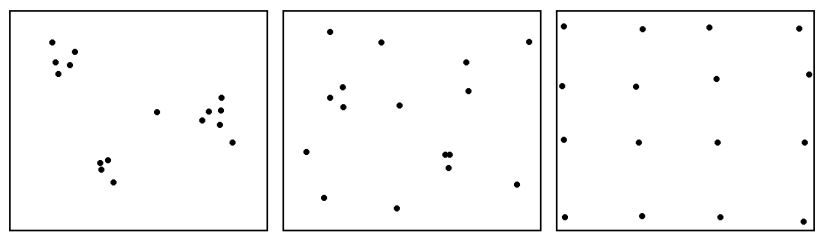
\includegraphics[width=0.9\linewidth]{../Imagenes/Patrones}
	\caption[Tipos de patrones espaciales]{ Agregado  (izquierda), Aleatorio (centro)  y    Regular (derecha) }
	\label{Patrones}
\end{figure}
	
	Un espacio que se caracteriza por la ausencia de estructura en la data, se dice que tiene aleatoriedad espacial completa (CSR, Complete Spatial Randomness, en inglés), su distribución teórica es conocida como la distribución de un proceso homógeneo Poisson, el Dr. Cressie señala que se puede considerar como el ruido blanco del proceso puntual espacial.
	
	En la próxima sección se define Aleatoriedad espacial completa o Proceso Homogéneo de Poisson.
	
	\subsection{Aleatoriedad espacial completa}
	
	
	
	De acuerdo con el marco teórico presentado por el Dr.Cressie, N. en su texto Stastiscs for Spatial Data, en el cual un patrón de puntos espacial con distribución Aleatorizada Espacial Completa (AEC) es tratado como un Proceso Homogéneo de Poisson (PHP), es decir, la aleatorización espacial completa es sinónimo de un Proceso Homogéneo de Poisson.\\
	
	
	
	\begin{defi}{Proceso Homogéneo de Poisson}	\label{Def_Poisson}	
		
		
		Un Proceso Homogéneo de Poisson, se caracteriza por las siguientes propiedades:
		
		
		\begin{enumerate}[i.-]
			
			\item El número de eventos  en una región acotada $ A \subset {\rm I\!R}^{2} $, con área $|A|$, sigue una distribución de Poisson   con media  $ \lambda |A|, $ donde $ \lambda $ es la intensidad del proceso (número de eventos por unidad de área).	
			
			\item  Dado $n$ eventos $\{s_{i}\}_{i=1}^{n}$ en la región $A$, estos son independientes con distribución uniforme sobre  $A$.
			
		\end{enumerate}
		
		
	\end{defi}
	

	Los procesos Poisson homogéneos representan el mecanismo estocástico más sencillo que puede generar un diseño puntual espacial;    a partir estos se construye la teoría de los procesos puntuales espaciales, y se aplican como modelo ideal de los procesos completamente aleatorios (Ramírez \cite{Ramirez}).\\
	
	Para describir el proceso consideremos una región acotada de ${I\!R}^{2}$. Digamos  $ A \subset {\rm I\!R}^{2} $, con área $|A|$, y sea \[ N(A) =  \: \text{ número de eventos  en  $A.$ }\]  De la condición $ii$, los $n$ eventos se distribuyen uniforme e independiente a lo largo del dominio $A$. La densidad condicional de la $n$-upla $ (s_{1}, s_{2},\dots, s_{n} ) \in   {\rm  A }^{n}$, dado $ N(A) = n $ es 
	
	
	\[f(s_{1}, s_{2},\dots, s_{n} ) = \frac{1  }{|A|^{n}  }  , \]  y de las condiciones  $i$ y $ii,$ la densidad conjunta para $n$ y   $ (s_{1}, s_{2},\dots, s_{n} )$ es dada por 
	
	\[   f((s_{1}, s_{2},\dots, s_{n} ),n) = \frac{ \lambda^{n} e^{-\lambda|A|}}{n!  }  \]
	
	En este caso la intensidad del proceso $\lambda(s) =\lambda $,   es homogénea en $A$; es decir,  la intensidad se asume constante a lo largo de la región en estudio (propiedad conocida como estacionaria). Intuitivamente, esto significa que los eventos tienen igual probabilidad de ocurrir en cualquier parte dentro de la región,  y además no interactúan unos con otros, es decir, no hay repulsión (regularidad de eventos), ni atracción (clúster de eventos) entre ellos (Cressie \cite{Cress}). Sin embargo, existen   procesos puntuales en que la distribución de la intensidad varía a lo largo de la zona de estudio; un modelo que se ajusta a esta característica es el proceso no homogéneo de Poisson, que  describe en la sección \ref{Poisson3}.\\
		
	
		
		El proceso puntual de Poisson homogéneo genera un punto de partida natural para la investigación estadística del patrón puntual observado. Bajo esta suposición se han planteado varios métodos para el probar la hipótesis nula (Cressie \cite{Cress}) de aleatoriedad espacial completa. En la sección \ref{AEC1} se describen algunas funciones empleadas para análizar esta situación.\\
		
		Un factor muy importante en el estudio del patrón de puntos espaciales, es la intensidad del proceso  $\lambda(\cdot)$, definida como la densidad igual al número de puntos por unidad de área; en la próxima sección se exponen algunos  métodos para estimar este parámetro. \\
		
		
		%   Pendiennte Definir:  \\
		%  A un proceso que es a la vez estacionario e isotrópico se le conoce como proceso homogéneo.
		%  Propiedad estacionaria\\
		%  propiedad estacionaria, esto es, la intesnsidad constante a lo largo de la zona de estudio .
		

		
		\subsection{Estimación de la intensidad}{\label{Estimacion}}		
		
		En el desarrollo del análisis espacial de los procesos puntuales es importante conocer la densidad del mismo en el área determinada, que representa la intensidad del proceso que lo ha generado. La intensidad es el número promedio de eventos ocurridos por unidad de área y se denota por: 
		
		\[ \lambda(s)  = \text{Número de eventos que ocurren por unidad de área}\].
		
		El problema de estimar la intensidad, en el caso de un proceso homogéneo de Poisson  consiste en estimar una función contante $ \lambda$, tal que el número esperado de eventos en la región $A \: (\int Adx)$  es igual al número de casos observados (Bivand  \cite{Roger}).   Una vez observado el proceso, se conocen las localizaciones de un conjunto de $n$ puntos; un estimador insesgado (ver sección \ref{Intensidad_Homogenea}) de la intensidad para este proceso está dado por \[ \hat{\lambda} = n/|A|,\] donde $|A|$ es el área de la región. Sin embargo, en el caso de un proceso no Homogéneo de Poisson la estimación debe ser tratada en forma diferente debido a la variación del parámetro. En la práctica, se emplean los métodos de la estimación no paramétrica, como la técnica o método de los cuadrantes, y la  técnica del kernel o suavizado  del kernel. Siendo la técnica del Kernel la más  recomendada   debido a la flexibilidad en los supuestos para la formación de función de densidad, pues estos no son tan rígidas como sucede en el planteamiento paramétrico de la estadística clásica.\\
		Los estimadores de tipo núcleo o kernel fueron diseñados para estimar la función de densidad de un conjunto de datos. La idea original es bastante antigua y se remonta a los trabajos de Rosenblatt (\cite{Devroye})  y   en la década del 50 y los primeros del 60. Los estimadores kernel son, sin duda, los más utilizados y mejor estudiados en la teoría no paramétrica. En el texto  A cuorse in Density Estimation de Luc Devroye (\cite{Devroye}), se definen mediante la expresión  $ \widehat{f}_{n}(s)  = \frac{1}{ nh_{n} } \sum_{i=1}^{n} k( \frac{ s -  s_{i}  }{h_{n}} ), $   donde $h_{n}$ es una sucesión de parámetros de suavizado, llamados ventanas o ancho de banda (windows, bandwidths), que deben tender a cero “lentamente” $(h_{n} \rightarrow 0, n h_{n} \rightarrow \infty)$ para  asegurar que   $\widehat{f}_{n}$ tiende a la verdadera densidad $f $  de la variable, y $k(\cdot)$ es una función de densidad prefijada llamada núcleo o kerne, que debe satisfacer ciertas condiciones de regularidad, como $ \int k(s) = 1, \:  \int s k(s) = 0,$  generalmente es una función de densidad simétrica alrededor de cero. En la practica, es muy  común usar la distribución normal estándar como la función  kernel o núcleo (función de densidad); es importante resaltar que las propiedades más importantes de estos estimadores no se ven afectadas por la función núcleo que se elija (Bivand  \cite{Roger}). \\
		
		
	A continuacón se expone la técnica del kernel para estimar la intensidad del proceso en caso de ser no homogéneo. 
	
		%	La intensidad puede ser constante (uniforme o Homogéneo) o puede variar de localización en localización (no homogéneo). La investigación de la intensidad debe ser uno de los primeros pasos en el análisis de patrones puntuales.
		
	
		
		
		
		%%%%%%%%%%%%%%%%%%%%%%%%%%%%%%% Función  Intensidad o medidad de intensidad  %%%%%%%%%%%%%%%%%%%%%%%%%%%%%%%%%%%%%%%%%%%%	
		
	
		
		
		\subsubsection{Estimación Kernel} \label{Kernel}
		
		
		Para  $n $ puntos dados  $ \{s_{i}\}^{n}_{i=1}$ en una región $A$, la forma de un estimador suavisado  kernel o núcleo para la intensidad,  el Dr. Cressie la describe mediante la siguiente expresión (Diggle \cite{Diggle}; Berman and Diggle, 1989)
		
		\[ \widehat{\lambda}(s)  = \frac{1}{ h^{2} } \sum_{i=1}^{n} k( \frac{ s -  s_{i}  }{h} )/\rho(s) \]  donde $ k ( \cdot ) $  es una función kernel simétrica bivariante,  $h$ el ancho de banda que  mide el nivel de suavización, y $ \rho(s) = \int_{A} k( \frac{ s -  u} {h}) du $ como una corrección de borde para compensar las observaciones perdidas que ocurre cuando $s$ está en el borde del área $A$. \\  
			

			{\bf{Ancho de banda}}\\  
			
	La elección correcta del parámetro de suavizado  $ h = h_{ n }$  es, sin duda, el problema más difícil en cuanto se plantea el método de estimación no paramétrica. En la actualidad existen varios procedimientos que permiten asignar $h$ de manera “optima” según  ciertos criterios de optimalizar que no se discutirán  en este trabajo (por ejemplo el método plug-in y
	el método de validación cruzada (Bivand  \cite{Roger}). 	
	
		 
 	
		 
		
		 Si el parámetro de suavizado se elige demasiado pequeño, el estimador aparece “infrasuavizado” (Bivand  \cite{Roger}) e incorpora demasiado “ruido”, reflejando  la presencia de muchas modas (máximos relativos) “espureas” que, de hecho no aparecen en la densidad que se quiere estimar. Por el contrario, si h se elige demasiado grande, se da el fenómeno contrario, de “sobresuavización” y el estimador es casi insensible a los datos. 
		 Esta situación se muestra en la  figura \ref{Ancho1y2Banda}, aplicado  a seis puntos con un kernel Gausianas y ancho de banda diferentes. La intensidad con la que cada punto influye en sus inmediaciones es igual para todos los puntos en este caso, y su alcance depende de la amplitud de la curva gausiana utilizada, es decir, el ancho de banda. Observe que en la función kernel resultante presenta un suavizado mayor (pierde detalles o información) con un ancho de banda mayor.\\
		
	\begin{figure}[h!]
		\centering 
	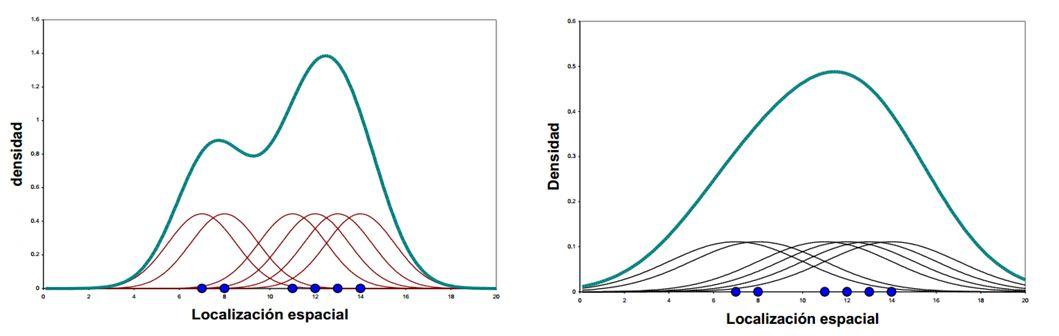
\includegraphics[width=0.75\linewidth]{../Imagenes/AnchoBanda1y2}
	\caption{Efecto de la selección del tamaño del parámetro de suavizado, sobre la estimación de la Intensidad.}
	 \label{Ancho1y2Banda}
\end{figure}
		En esta investigación el método para seleccionar ancho de banda implica un procedimiento de ensayo y error, hasta aproximarse al grado de resolución deseado.   Sin embargo, el software R, ofrece técnicas para calcular este parámetro. El paquete (o librería) Spatstat tiene el comando o código { \ttfamily {adaptive.density()}} (Baddeley\cite{Badbeley}),  para obtener la estimación de la intensidad con un ancho de banda “adaptativo”. En el mismo se establece el número de puntos vecinos a tener en cuenta para el cálculo.  Así, en regiones de alta densidad el cálculo se realiza a partir de puntos cercanos, mientras que en zonas de pocos puntos, se obtiene a partir de observaciones más distantes.\\
		
		 	
		 %	A continuación, veremos varios procedimientos de estimación de h o también 	denominados selectores del ancho de banda o métodos se selección de la complejidad del modelo
		 
		
		
		\section{Métodos para verificar aleatoriedad espacial completa}{\label{AEC1}}
		
		
		En el proceso puntual homogéneo de Poisson en general, se asume que la intensidad es constante a lo largo de la zona de estudio ( propiedad conocida como estacionaria). Sin embargo, existen distribuciones como la distribución no homogénea de Poisson que presenta variabilidad de la intensidad a lo largo de la zona de estudio.  La metodología que se emplea en este trabajo para analizar la aleatoriedad espacial completa  del patrón  de puntos del fenómeno espacial, consiste  en  comparan de  las propiedades de primer orden  y las denominadas propiedades de segundo orden, con las de la distribución teórica.		
		
		Las propiedades de primer orden, se basan en la intensidad del proceso $\lambda(h)$, que es definida como la densidad; es decir, el número de puntos por unidad de área (Olaya \cite{Olaya}).   Mientras que las propiedades de segundo orden, toman en cuenta la distancia entre puntos, y estudia las posibles relaciones entre cada punto con los de su entorno.  \\
		
		Es importante señalar, que tanto la intensidad como la densidad espacial son parte de las propiedades de primer orden, pues ni la intensidad ni la densidad dan información sobre interacción entre dos puntos cualquiera; ellas miden la distribución de eventos en la región de estudio. La interación es medido por las propiedades de segundo orden, el cual reflejan cualquier tendencia de los eventos como clúster, independencia o regularidad espacial  (Bivand  \cite{Roger}).  \\
		
		
		A continuación se presentan una descripción de los estadísticos  para probar la aleatoriedad espacial completa del proceso, basadas una técnica de cuadrantes y  de la distancias.
			
	
		\subsection{Método basados en cuadrantes}\label{MCuadrantes}
		
		El método basados en cuadrantes para describir la aleatoriedad espacial de un patrón de puntos, consiste en particionar el dominio $ A$ en subregiones, digamos $ B_{1}, B_{2},\dots , B_{k} $ tal que  $  \cup_{i=1}^{k}  B_{i}  =  A$, y no se traslapen  $( \: B_{i} \cap B_{j} = \emptyset$). Estas pueden tener forma irregular, pero la más común es la rectanguar o unidades cuadradas, de aquí el nombre de cuadrantes. El Dr. Cressie hace una presentación del método usando  círculos  distribuidos en forma aleatoria sobre la región. Sin embargo, en esta investigación se emplea  el método de los cuadrantes regulares sobre una rejilla o grilla. Una vez definido el número de rejillas, se cuenta el número de puntos que aparecen dentro de cada cuadrícula. Con los datos $n_{i, j}$ obtenidos del conteo de puntos o eventos dentro de cada cuadrícula, se procede al análisis estadístico. Este se lleva a cabo comparando los conteos en los cuadrantes y aplicando el estadístico Chi-$\chi^{2}$ (test de bondad de ajuste),  o mediante la relación entre la media y la varianza de la data, indice de varianza relativo $I$ (índice de Fisher 1922, Cressie \cite{Cress}). En el segundo caso, partimos de que la distribución aleatoria teórica esperada debe tener varianza igual a la media. Por tanto, el cociente entre la varianza y la media debe ser cercano a 1. Si el cociente está próximo a ese valor, se tratá de una distribución aleatoria. Si el patrón de la distribución es uniforme, la varianza  será cercana a 0, y por tanto el cociente con la media es cero. En las distribución agrupadas, la varianza será mayor, y el cociente por tanto superior a 1. También se usa el índice  ICS $ = (I - 1)$ (David y Moore  1954){\footnote{Cressie, N. , 1993, Stastiscs for spatial data}}.\\
		
		En la prueba de bonda de ajuste Chi-$\chi^{2}$, la hipótesis nula asume que los n puntos son distribuidos uniformemente independientes a lo largo de $A$; en otras palabras, los conteos de sitios por cuadrante son variables Poisson independientes con media común.
		Este estadístico  está dado por la expresión
		
		
		\[ X^{2} =\sum_{i=1}^{r} \sum_{i=1}^{c}  \frac{(O_{i, j} - E_{i, j})^{2} }{ E_{i, j} } \: \text{ Vs } \: \chi^{2 }_{(r c -1)} \] donde $O_{i, j} = n_{i, j } $,  	 $ E_{i, j} = \frac{n_{\cdot,j} n_{i,\cdot}}{n} = \frac{n}{rc} .$\\ 
		
		Si  $N(A) =  $ número de puntos en  $A,$ tiene distribución de $ Poisson(\lambda|A|)$, entonces la  $ \widehat{ V}(N(A)) \approx \widehat{E}(N(A)),  \text{ y con el estimador de} \: \lambda, \: $ como $ \: \widehat{\lambda} = \frac{n}{|A|} $
		
		\[  \:  \Rightarrow  \: 
		X^{2} =\sum_{i=1}^{r} \sum_{i=1}^{c} \frac{(O_{i, j} - E_{i, j})^{2} }{ E_{i, j} }    \:
		\approx  \: \chi^{2 }_{(r c -1)} \] Índice de dispersión \[I =  \frac{\widehat{V}(N(A))}{ \widehat{ E}(N(A))} \approx 1 \] Índice de tamaño del clúster: $  (I - 1)$\\ 
		
		\begin{displaymath}
		(I - 1)=\left\{ \begin{array}{rcl}
		\approx 0  &\text{patrón es aleatorio,}\\
		>   0      &\text{patrón es agregado,} \\
		<   0      &\text{patrón es regular}.
		\end{array}
		\right.            
		\end{displaymath}  \\       {\bf{Desventajas del método:}} \\
		
				
		El análisis por cuadrantes no es en realidad una medida del patrón, sino de la dispersión. Además, presenta algunos inconvenientes, como el efecto de escala que tiene gran influencia en los resultados obtenidos; el uso de la unidad de análisis fija (el cuadrante), puede no ser capaz de localizar agrupamientos locales en ciertas áreas.
		
			\begin{figure}[h]
			\centering
			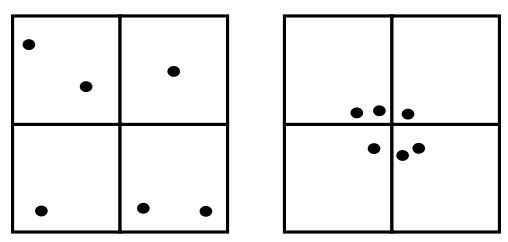
\includegraphics[width=0.7\linewidth]{../Imagenes/Desventaja}
			\caption{Dos disposiciones de puntos distintas que darían un mismo resultado al analizarse por el método de cuadrantes}
			\label{Desventaja}
		\end{figure}
		
	
		
		 Por otro lado, el método no es capaz de diferenciar entre distribuciones tales como las de la figura \ref{Desventaja}, claramente distintas pero que arrojan un resultado idéntico al aplicar esta metodología con los cuadrantes mostrados. No obstante, la aplicación de este método en campos como en ecología y biología es muy habitual, y se han desarrollado numerosas extensiones del mismo tales como el  índice de David–Moore,  el  índice  de  frecuencia  de  agregados,  o el índice  $I_{\delta}$  de Morisita(1959){\footnote{Cressie, N. , 1993, Stastiscs for Spatial Data}},   entre otros muchos.\\
		
	
	Bajo la hipótesis de AEC, las $n_{i, j}$ variables de Poisson son independiente e idénticamente con el mismo valor esperado. Y se puede usar el  $X^{2}$  Pearson para la prueba del buen ajuste ( Baddeley \cite{Badbeley}).
	
			
		%  El mismo proveen  objetos y algoritmo que permiten calcular las funciones  F, G, K, L; funciones que se emplean para  describir la edad espacial completa descritas en la sección (\ref{funciones}). \\
		
		
		\subsection{Métodos basados en distancias}\label{funciones}  
		
		
		Para probar la hipótesis de aleatoriedad basados en conteos por áreas, la elección de la forma y el número de cuadrantes  es un elemento que puede influenciar los resultados. Las pruebas estadísticas basadas en distancias entre eventos o entre puntos muestreados 	y eventos  permite solventar algunos de los problemas asociados al análisis de cuadrantes. Además, estos métodos dan mayor información  y permiten medir la incertidumbre relacionada con patrón (Cressie \cite{Cress}) . En esta sección se describen algunas funciones y métodos que tienen en cuenta la distancia entre eventos o puntos muestreados. \\
		
			
		\subsection*{Función $G$:} Distancia del vecino más cercano (Cressie \cite{Cress}).  La función $G(d)$ mide la probabilidad de que las distancias de un evento arbitrario (seleccionado al azar)  a sus vecinos más cercanos sea menor o igual $d$. De esta forma la distancia en términos de variable aleatoria $ D $, es definida como la distancia del evento arbitrario $i$ al sitio del evento más (Bivand \cite{Roger}), es decir,		
		 \[ D = \text{distancia del evento arbitrario}  i  \text{ al sitio del evento más cercano} \]
		
		Si la distancia se define como $d_{i}= min_{j}\{d_{ij}, \forall j \neq i\},  i = 1, . . ., n, $  donde  $d_{i}$ es la mínima distancia entre del evento $ i$ y sus vecinos.  La Función de distribución empírica $G(d)$ de $D$,  es definida por  
		
		
		\[\widehat{G}(d) = \frac{\#\{di : di \leq d , \forall i \}}{n}\]  donde el numerador es el número de elementos del conjunto de distancias que son menores o iguales a d,  y n es el número total de punto (Cressie \cite{Cress}).\\
		
		
		
		
		Bajo aleatoriedad espacial completa en ${I\!R}^{2}$, el valor de la función $G(\cdot)$está dado por
		
		\[ G(d) = P (D \leq d) = 1 -e^{- \lambda \pi d^2 } \]  donde $\lambda $  representa de número el promedio de eventos por unidad de área o la intensidad  (Cressie \cite{Cress}) .\\
		
		
		
		%    $ G(d) = P (D \leq d) = 1 - P (D > d) = 1 – P($No hay eventos en $ A =\pi d^2) = 
		%    1 - exp\{-\lambda \pi d^2\}${\footnote{  Matern, 1971, en Cressie pag 614}},
		%    Por ejemplo si $N(A)$ representa el número de eventos en $ A, i = 1, 2,\dots , n$, seleccionados al azar.
		%    Claramente   $N(A)  Poisson(\lambda^2)${\footnote{ colombiano, Cressie613 y texto R espacial 182}}. Entonces $P (N(A) = 0) = %    e-\lambda \pi d2$     por lo tanto  $G(d) = 1 – e-\lambda \pi d2$.
		%                $ \lambda(|A|)$ 
		
		% ###################### spatstat functions ###################### 
		% The next chunk of code shows how to compute this by using spatstat functions Gest   161 o 167
		
		Para comparar el patrón observado con un patrón bajo AEC, se grafica la función $\widehat{G}$ estimada  contra la función teórica; además se puede simular el proceso con la intensidad del patrón observado sobre área de estudio (Diggle \cite{Diggle}), y verificar si la función empírica está dentro del intervalo (Bivand  \cite{Roger}).\\
		
		% {\footnote{Roger S. Bivand • Edzer J. Pebesma Virgilio Gómez-Rubio Applied Spatial Data Analysis with R, Springer, pag 167}}
		
		La función $G(d)$  describe el proceso como: 
		
		\begin{enumerate}[$\bullet$]
			
			\item  Si $\widehat{G}(d)$ crece rápidamente en distancias cortas, los eventos son agregados.
			
			\item  Si  $\widehat{G}(d)$ crece lentamente hasta cierta distancia(espacio eventos) y después crece rápidamente, los eventos son regularmente espaciados.
			
		\end{enumerate}
		
		\subsubsection{Bandas de confianza}
		Adicionalmente se hace un cálculo de las bandas de confianza  para la función en donde se
		calcula:
		
		
		Los gráficos pendientes.  
		
		\begin{enumerate}[a.-]
			
			\item  $\widehat{G}(d)$ = Función $G(d)$ calculada con los datos observados
			
			\item  $\widehat{G}_{1}(d), \widehat{G}_{2}(d), \dots  \widehat{G}_{m}(d)$ = Función $G(h)$  calculada con $m$ realizaciones de un proceso completamente aleatorio.   
			
			\item  $G_{L}(h) = min_{j}\widehat{G}_{i}(h)$     y    $G_{U}(h) = max_{j} \widehat{G}_{i}(h)  $
			% i=1,..,m,                              i=1,..,m  
			
		\end{enumerate}
		
		
		
		\subsection*{Función F:} Distancia de un punto arbitrario, al evento más cercano (Cressie \cite{Cress}).  Esta función tiene en cuenta la mínima distancia punto-evento, donde un punto es  escogido aleatoriamente dentro de la región en estudio. La función mide la distribución de todas las distancias del punto arbitrario en el área y su evento  más cercano. Esto es, la distancia mínima punto-evento, donde un punto es  escogido al azar  dentro de la región de estudio. Así, la variable aleatoria $D$, es define como la distancia del punto al   evento  más cercano, \[ D  = \text{ mínima distancia de un punto a un evento}.\]   La distribución  empírica $\widehat{F}(d)$ de $D$,  dada por  
		
		\[ \widehat{F}(d) = \frac{\#\{d_{j} : d_{j} \leq d , \forall j\} }{m}\]     Bajo AEC su distribución teórica (Cressie \cite{Cress}) está dada por:             
		
		\[ F(d) = 1 - e^{-\lambda \pi d^{2}} \] 
		
		
		
		
		Para calcular este estadístico se siguen los siguientes pasos:
		
		\begin{enumerate}[a.-]
			
			\item   Se seleccionan  al azar $m$ puntos   ${  p_{1},  p_{2},  \dots , p_{m} } $, dentro del área.
			
			\item   Se calcula $d_{j} = d(p_{j}, s_{i})$, la distancia de cada punto seleccionado al sitio $s_{i}$ del evento más cercano.
			
		\end{enumerate}
		
		
		
		
		El proceso es descrito por la función $\widehat{F}(d)$   como sigue: 
		
		\begin{enumerate}
			
			\item   
			Sí $\widehat{F}(d)$ crece lentamente al comienzo y rápidamente para distancia largas, el patrón es agregado.
			
			\item   
			Sí $\widehat{F}(d)$  crece rápido al comienzo, el patrón es regular.
			
		\end{enumerate}
		
		
		
		Bajo aleatorización espacial completa  la función de distribución de G(Y) y F(Y) son iguales (Cressie \cite{Cress}).
		
		
		%%  pag 171 7.4.5 Second-Order Properties ( R con estadis)
		
		
		
		
		%%%  Gráficos pendientes
		%%   Para traducir 
		%%   This function is often called the empty space function because it is a measure of the average 
		%%  space left between events.
		
		%%  La function K de Ripley An alternative way of measuring second-order %%   properties when the spatial process is  HPP          %% is  by  means of the      K-function (Ripley, 1976, 1977).
		
		
		
		
		\subsection*{Función K:} El estadístico k de Ripley (1976) es un indicador de la no aleatoriedad medida en diferentes escalas de valores o diferentes regiones; el estadístico mide el tipo de interacciones entre los eventos del proceso, particularmente clúster o regularidad entre eventos. También es llamado medida de reducción de segundo momento, insinuando que ha sido diseñado para medir la tendencia segundo-orden, es decir, de clúster local. Sin embargo, este estadístico también está sujeto a los efectos de primer orden; en sentido, de que no indica donde ocurre el clúster, así que no es estrictamente una medida de segundo orden (Cressie \cite{Cress}).\\
		
		% Ned Levine y Cressie        Ned Levine Crimen Stat, Cressie(1993)
		
		
		%%  La intensidad λ se anade para eliminar la influencia de la densidad, ya que el valor esperado
		%%  de puntos a una distancia dada está en relación directa con dicha densidad.  tomado del Libro del SIG 
		
		
		
		La función $K$ de Ripley mide el número de eventos que se encuentran dentro de una distancia dada a cualquier evento particular. En términos de variable aleatoria, para una distancia $h$ se escribe como:
		\[ K(h) = \lambda^{-1} E[N(h)] \] 
		donde $N(h)$  representa el número de  eventos dentro de la distancia $h$ alrededor de un evento  cualquiera (aleatorio),    $E[N(h)]$ valor esperado de  $N(h)$, y $\lambda$ la intensidad (Cressie \cite{Cress}).\\
		
		Para calcular esta función, Ripley (1976) propuso un estimador insesgado igual a 
		\[ \widehat{K}(h) = \frac{1}{\lambda^{2} |A|}\sum_{i}^{N}\sum_{j, j\neq j}^{N} I_{h}(d_{i,j} ) \] siendo  $ I_{h}(\cdot) $ 
		la función indicadora definida como
		
		\[ I_{h}(d_{i,j}) =  \left\{ \begin{array}{rcl}
		1 & \text{ si} \:\:  d_{i,j} \leq h \\
		0 &\text{ si} \:\: d_{i,j} >  h\\
		\end{array}
		\right.  \] 
		
		En este estimador no se consideran los efectos de borde, y aquellos puntos situados cerca
		de la frontera de la zona de estudio tendrán estimaciones inferiores a las reales. Un estimador
		que corrige los efectos de borde es el siguiente:
		
		
		\[  \widehat{K}(h) = \frac{1}{\lambda^{2} |A|} \sum_{i}^{N}\sum_{j, j\neq j}^{N}\frac{I_{h}(d_{i,j} )}{w_{i,j}} \] donde $w_{i,j}$  pondera los distintos puntos en función de su distancia al borde de la zona de estudio. Para calcularlo se traza una circunferencia por el punto $i$ con radio $d_{ij}$ (es decir, una circunferencia con centro en el punto $i$ y que pasa por el punto $j$), siendo $w_{i,j}$  la fracción de dicha circunferencia que queda dentro de la zona de estudio, ver figura \ref{Correccion}.
				
		Puesto que la densidad se estima como $\lambda = \frac{N}{|A|}$, la expresión del estimador de la función $K$  queda finalmente expresado como: 
		
		\[  \widehat{K}(h) = \frac{|A|}{N^{2}}\sum_{i}^{N}\sum_{j, j\neq i}^{N}\frac{I_{h}(d_{i,j} )}{w_{i,j}} \]
		
		
		
		Para interpretar el significado de la función $K$, se tiene que, en condiciones de aleatorieda
		espacial completa en ${I\!R}^{2}$, el número de eventos a una distancia menor que $h$ es $\pi h^{2}$ (es decir,  $K(h) = \pi h^{2}$). Comparando los valores esperados con los estimados, se tiene que  sí  $ \widehat{K}(h) < K(h) $  existe agrupamiento; mientras que sí  $ \widehat{K}(h) > K(h)$ existe regularidad en la distribución.
		
		
		\begin{figure}[h]
			\centering
			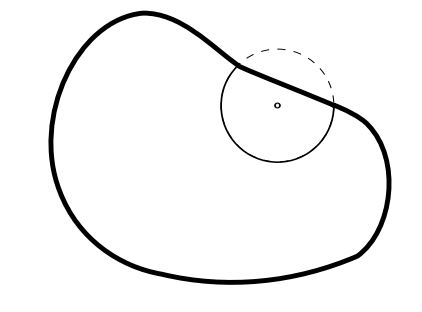
\includegraphics[width=0.35\linewidth]{../Imagenes/Correccion}
			\caption{Corrección del estimador $ \widehat{K}(h)$ en función de los efectos de borde. El parámetro de
				corrección es el cociente entre la longitud interior (en trazo continuo) y el total de la circunferencia}
			\label{Correccion}
		\end{figure}
		
		
		
		
		
		
		\subsection*{Función $L$:} 	Para facilidad de interpretación resulta habitual utilizar un estimador  $\widehat{L}(h)$, llamado  función $L$, así, 
		
		\[  \widehat{L}(h) = \sqrt{ {\frac{\widehat{K}(h)}{\pi} }}- h \] de tal modo que valores positivos de  $\widehat{L}(h)$ indican agregación, mientras que los negativos indican regularidad.\\
		
	                   
		
			%%  Además de comparar el valor estimado con el valor esperado de la función $K$ en condiciones de aleatoriedad espacial completa, puede compararse con el esperado para un proceso puntual determinado.
		
		
		
		
		
		%   Al igual que los métodos restantes, el empleo de funciones $K$ se realiza con carácter
		%   global, asumiendo la estacionaridad de la función K(h). No obstante, puede adaptarse a un
		%   uso local, considerando en lugar de una serie de puntos aleatorios, un punto concreto i.
		
		
		%%%%%%%%%%%%%%%%%%%%%%%%%%%%%%%%%%%%%%%%%%%%%%%%%%%%%%%%%%%%%%%%%%%%%%%%%%%%%%%%%%%%%%%%%%%%%%%%%%%%%%%%%%%%%%%%%%%%%%%%%%%%%%%%
		%%%%%%%%%%%%%%%%%%%%%%%%%%%%%%%%%%%%%%%%%%%%%%%%%%%%%%%%%%%%%%%%%%%%%%%%%%%%%%%%%%%%%%%%%%%%%%%%%%%%%%%%%%%%%%%%%%%%%%%%%%%%%%%%
		
		
		
		
		\section{Modelos de Procesos Puntuales} 
		
		
		La pruebas de aleatoriedad espacial completa es sólo el primer paso en el análisis de espacial de patrones puntuales, si la hipótesis nula  es rechazada el próximo paso es ajustar algún  modelo alternativos a la data. Generalmente la desviación de la AEC  lleva a un patrón  caracterizado por clúster o regularidad.  El Dr. Cressie expone algunos modelos que pueden ser ajustados a cada situación. Así, el clúster puede ser explicado a través del modelo no homogéneo de Poisson, por el  Proceso de Cox o por el proceso  de Poisson con clúster ; y el modelo simple inhibición puede ser usado para modelar el patrón de puntos regular.   El proceso puntual marcado puede incorporar ambos elementos,  a través de escala-pequeña  para regular y escala-grande para clúster.  \\
		
		
		A continuación se describen algunos de estos modelos alternativas para procesos regulares y agregados.\\
		
		% 
		
		
		\subsection{Modelo de Poisson  homogéneo}{\label{Poisson4}} {\label{Intensidad_Homogenea}}
		
		Los procesos homogéneos de Poisson son la base fundamental en que se construye la teoría de los procesos puntuales espaciales, se aplican como modelo ideal de los procesos completamente aleatorios, y por supuesto que  muchos procesos puntuales se adaptan a este modelo.   En este caso la intensida es constante, esto es:  $ \lambda(s) = \lambda$, para todo $s\in A$.
		
		Dado $N(A) = n$,  la $n$-upla $ (s_{1}, s_{2},\dots, s_{n} ) \in   {\rm  A }^{n} $  está  distribuida como una muestra aleatoria  independiente sobre $A$ con densidad de probabalidad proporcional a $\lambda(s)${\footnote{Cressie, N. , 1993, Stastiscs for Spatial Data}}. Esto es,   
		
		
		
		
		
		\[   \lambda(A) = \: \int_{A} \lambda(s) ds = \int_{A} \lambda ds = \lambda\int_{A} ds = \lambda |A|\]
		
		% con media   \mu(A)= E( N(A) ) =
		
		
		\[P [ N(A)  = n] =  \frac{ (\lambda|A|)^{n} e^{-\lambda|A| }}{n!  } \]   
		
		
		
		%   La Intensidad o función intensidad (\ref{Intensidad1})  de $N(A)$,    $  \lambda(s) = \lim_{  |ds| \rightarrow   0} \frac{ E( N(ds) ) }{ |ds| } . $ 
		
		\[f_{A}(s|n ) = \frac{\lambda(s)  }{ \int_{A} \lambda(u) du  }  = \frac{\lambda  }{ \lambda|A| } = \frac{1 }{ |A| }, \: \:  s \in A\]   y de las condición $i$ y $ii$,  la densidad conjunta  de $ (s_{1}, s_{2},\dots, s_{n} )$  y $n$ esta dada por 
		
		
		
		
		\[f(s_{1}, s_{2},\dots, s_{n}| n ) = \frac{ \Pi^{n}_{i=1}\lambda(s_{i})  }{( \int_{A} \lambda(u) du )^{n} } = \frac{1 }{ |A|^{n} } \]  y
		
		% \[  \mu(A)= E( N(A) ) = \lambda(A) = \: \int_{A} \lambda(u) du, \] número de eventos en promedio que  se espera  aparecen en $A$.\\
 
		
		\[f(s_{1}, s_{2},\dots, s_{n}, n ) = \frac{1 }{ |A|^{n} } \frac{ (\lambda|A|)^{n} e^{-\lambda|A| }}{n!  } =  \frac{ \lambda^{n} e^{-\lambda|A| }}{n!  } \] 	aplicando $ln(\cdot)$ 
		\[ ln(f(s_{1}, s_{2},\dots, s_{n}, n )) =   -\lambda |A| + n \: ln(\lambda) - ln(n!)   \] y derivando 
		\[ \frac{ d\, (ln f_{A})}{d \lambda } =   - |A| +\frac{n}{\lambda}  =0 \] obtenemos el estimador insesgado  de máximo verosímil para la intensidad  dado por:  \[\hat{\lambda} =\frac{n}{|A|} \]   Sin embargo,  existen procesos puntuales espaciales que no se ajustan a este modelo; quizás el modelo alternativo al modelo HPP más simple,  es el proceso de Poisson no homogéneo (proceso no  estacionario),  que se obtiene sustituyendo la intensidad constante en la región $A$,  por   $\lambda(s)$, que  puede ser el resultado de variaciones estocásticas en la región $A$. En este sentido, si se quieren modelar fenómenos donde la distribución espacial de los eventos puede ser el resultado de variaciones estocásticas, es razonable pensar en la función de intensidad de un proceso de Poisson   $\lambda(s)$,  como una realización de un proceso estocástico.
		
		
		\subsection{Modelo de Poisson no homogéneo}{\label{Poisson3}}
		
		El modelo o proceso no homogenéo de Poisson (PNP) considerado como la alternativa al modelo de Poisson homogéneo mas simple, pués la diferencia entre ámbos procesos es que el PHP asume la intensidad como una función constante en toda la región $A$, mientras que el PNP la intensidad se considera  una función variable a lo largo de la zona de estudio. Esta analogía se puede expresar indicando que el proceso no homogéneo de Poisson es una generalización del proceso homogéneo de Poisson, o al contrario.
		
		Como ejemplo de un proceso con está característica tenemos la distribución de la población en una ciudad, y la población de alguna especie árboles en un bosque, en ámbos casos la distribución se ve afectada por  factores propios de cada fenómeno. \\
		
		
		El proceso no homogéneo de Poisson se define como:
		
		
		\begin{defi}{Proceso no Homogéneo de Poisson}
			
			Un Proceso no  Homogéneo de Poisson{\footnote{Cressie, N. , 1993, Stastiscs for Spatial Data}}, se caracteriza por las propiedades:
			
			\begin{enumerate}[a.-]
				
				\item El número de eventos  en una región $ A \subset {\rm I\!R}^{2} $, con área $|A|$, sigue una distribución de Poisson   con media  $ \lambda(A) $, donde $ \lambda(A) $ la intensidad del proceso depende de la localización espacial.
				
				\item  Dado $n$ eventos $\{s_{i}\}_{i=1}^{n}$ en la región $A$, éstos son independientes y  distribuidos uniformemente sobre $A$.
				
			\end{enumerate}
			
			
		\end{defi}
		
		
		
		Siguiendo la analogía dada en el proceso de Poisson homogéneo. \\ 
		Sea $ A \subset {\rm I\!R}^{2} $,  una región acotada  de  área $|A|$, y sea \[ N(A) =   {\text{ número de eventos  en  $A$}}.\] En este caso la intensidad  esta  determinada por la función de localización espacial  $\lambda(s)$;  pués  no es proporcional al área  $A$ como en el caso PHP. \\
		
		
		De la definión \ref{Def_Poisson} del proceso de Poisson  y como consecuencia el proceso  puntual $N(A)$ se satisface 
		
		
		\[P [ N(A)  = n] =  \frac{ \lambda(A)^{n} e^{-\lambda(A) }}{n!  } \] con media  
		
		\[  \mu(A)= E( N(A) ) = \lambda(A) = \: \int_{A} \lambda(u) du, \]
		número de eventos en promedio que  se espera  aparecen en $A$.\\
		
		
	%	La Intensidad o función intensidad ( \ref{Intensidad1} )  de $N(A)$,    $  \lambda(s) = \lim_{  |ds| \rightarrow   0} \frac{ E( N(ds) ) }{ |ds| } . $ 
		
		 Dado $N(A) = n$,  la $n$-upla $ (s_{1}, s_{2},\dots, s_{n} ) \in   {\rm  A }^{n} $  está  distribuida como una muestra aleatoria  independiente sobre $A$ con densidad de probabalidad proporcional a $\lambda(s)$. Esto es,   
		
		
		\[f_{A}(s ) = \frac{\lambda(s)  }{ \int_{A} \lambda(u) du  }, \: \:  s \in A\] De aqui, la densidad condicional de la $n$-upla $ (s_{1}, s_{2},\dots, s_{n} ) \in   {\rm  A }^{n}$, dado $ N(A) = n \: \:  $   es 
		
		
		\[f(s_{1}, s_{2},\dots, s_{n} ) = \frac{ \Pi^{n}_{i=1}\lambda(s_{i})  }{( \int_{A} \lambda(u) du )^{n} }  \] y de las condición $i$ y $ii$ la densidad conjunta   $ (s_{1}, s_{2},\dots, s_{n} )$  y $n$ esta dada por 
		
		
		
		
		\begin{displaymath}
		f((s_{1}, s_{2},\dots, s_{n} ),n ) = \left\{ \begin{array}{rcl}
		e^{-\lambda(A)},         & n  =  0  \\
		\frac{ e^{-\lambda(A)}  \Pi^{n}_{i=1} \lambda(s_{i}) }{n!} & n\geq 1 \\
		\end{array}
		\right.            
		\end{displaymath}
		
		
		
		La intensidad $\lambda(s) $  no es homogénea, significa que la ocurrencia de eventos depende de la localización  en la región; además pueden que los eventos  interactúan unos con otros, es decir, pueden presentar  repulsión (regularidad de eventos), o atracción (clúster de eventos) entre ellos,  situación que  dependen del fenómeno (Cressie \cite{Cress}).  \\
			
			Una vez observado el proceso se tienen las localizaciones de los $n$ eventos, en el caso del un PHP un estimador insesgado de la intensidad del proceso es $n/|A|$, donde $|A|$ es el área de la región, esto asegura que el número esperado de puntos es el número observado de puntos. Sin embargo, para un PNP la estimación de la intensidad debe ser desarrollada en forma diferente. En este caso puede ser calculada mediante la estimación no paramétrico empleando el método suavización del kernel o por el método paramétrico de una función específica cuyo parámetro es estimado por el método de máxima verosimilitud de los posesos puntuales (Bivand  \cite{Roger}). \\
		
	En este trabajo se emplea la técnica  del kernel  para estimar intensidad del proceso no homogéneo (Ver sección \ref{Estimacion}). 
		
		%%	Proceso Poisson no homogéneo.\\	El modelo más simple cuando el proceso no es estacionario es el proceso de       Poisson no homogéneo, que se obtiene sustituyendo la intensidad constante $\lambda$, de un proceso de Poisson por una			función de intensidad variable $\lambda(x)$. Un proceso de Poisson es no homogéneo si: 			1. Si $N(A)$ representa el número de eventos en $A \subset D$,  entonces $ N(A)$ $\equiv$   $Poisson(\lambda(A) )$ con 	$	0 \le \lambda(s) < \infty$  	2. Si $ A_{1} $ y $A_{2}$ son disyuntos, entonces $N(A1) $ y  $N(A2) $  son independientes 		3. La probabilidad de  $s \in A$ es proporcional a la función $\lambda(s)$  		\[f_{A}(s) =  \frac{\lambda(s)}{\int_{A} \lambda(s)ds}\]
			
			
			\subsection{Proceso de Cox}{ \label{Cox1} } 
			
			De manera informal un proceso de Cox es un proceso no homogéneo de Poisson, con media o intensidad  aleatoria. El Dr. Cressie ilustra el  proceso de Cox con el siguiente ejemplo.\\
			
			Sea $A$ una región acotada, y suponga que puede ser particionada en $k$ subconjuntos disjuntos $ \{ A_{1}, A_{2}, \cdots,  A_{k} \} $,  tal que los eventos en cada $ A_{i} $ son una realización de un proceso homogéneo de Poisson con intensidad $ \lambda_{i} \: $,  donde $ \lambda_{1}, \lambda_{2},\cdots, \lambda_{k} \: $ son variable aleatorias independientes e identicamente distribuidas. Entonces el proceso espacial de puntos que resulta es un Proceso de  Cox (Cox y Isham. 1980) (Cressie \cite{Cress}). En este caso $ \{ \lambda_{i}  \}^{k}_{i=1}$, es una realización de un proceso estocástico  sobre $A$.			
			
			Este modelo de proceso ha sido empleado frecuentemente en el análisis de fenómenos ecológicos (Cox o Gibbs), tales como  distribuciones  de masas forestales (Olaya \cite{Olaya}).\\
						
			
			El proceso de Cox se define como:
			
			\begin{defi}{Proceso de Cox}{ \label{Cox2} }
				
				El Proceso  puntual $N(A)$ es un proceso de Cox{\footnote{Cressie, N. , 1993, Stastiscs for Spatial Data}} sí, $N(A)$ es un proceso no homogéneo de Poisson, donde  la función intensidad es aleatoria.
				
			\end{defi} 
			
			
			
			La intensidad  del proceso de Cox se expresa por 
			
			\[  N(A) = \int_{A} \Lambda(s)ds \] donde  $ \Lambda(s) $ es una variable aleatoria generalmente distribución Gamma (en este caso el número de eventos   del proceso en $A$ es aleatoria, y la intensidad se puede expresar como:  $\lambda(s)  =  \Lambda(s)$ ).\\
			
			{\bf {Proceso de Poisson / Gamma\\
					
					$ \lambda(s) \approx $ Gamma($\alpha, \beta $)
					
					\[ f( \Lambda(s) )  =   \frac{ 1  }{  \beta^{\alpha} \Gamma( \alpha )  } \lambda(s)^{\alpha -1} e^{( \frac{-\alpha(s)}{\beta} )}  \]
					
					
					\[ E ( \Lambda(s) )  = \alpha  \beta,  \: \:  \: \:  Var( \Lambda(s) )  = \alpha  \beta^{2}    \]    }}
			
			
			
			
			
			
			\subsection{Proceso de Poisson con  Clúster}{ \label{Pcluster1} }
			
			
			Los procesos de Poisson con clúster son modelos que incorporan explícitamente la formación de grupos y por tanto, proporcionan la base adecuada para modelar patrones
			puntuales con eventos agrupados (Cressie \cite{Cress}).\\
			
			
			Son procesos que cumplen las siguientes condiciones:
			
			
			\begin{enumerate}[i.-]
				
				\item  Hay un proceso con padres  que siguen un proceso no homogéneo de Poisson con intensidad $ \lambda_{p}$.
				
				\item  Cada padre produce un número aleatorio de descendientes de acuerdo a una
				distribución.
				
				\item  Las posiciones de los descendientes respecto a los padres es aleatorio y sigue una
				distribución bivariada.
				
				\item  El proceso final,  proceso Poisson-Cluster corresponde sólo a la  posición de los descendientes.
				
			\end{enumerate}
			
			
			%%   Nota: Si $f(s)$ es una normal bivariada, el proceso se llama Thomas  tiene función K
			%%   conocida. \[  f(x, y) = \frac{1}{\sqrt{2}  \pi \sigma } exp\{ \frac{ x^{2} + y^{2}}{2 \sigma^{2}}\} : \: \: \: \:  k(h) = \pi %%   h^{2} + (\frac{1+exp(\frac{-h^{2}}{4\sigma^{2}})}{\lambda}) \]  La estimación de los parámetros ($\lambda$  y $\sigma^{2}$) se hace por la minimización de la función de  contrastes.
			
			
			
			\subsection{Proceso de Inhibición Simple (MATERN I)}{ \label{Pcluster1} }
			
			
			
			Los modelos alternativos al de Poisson presentados hasta ahora tienden a producir diseños agrupados.  Para describir un patrón regular de puntos la forma más natural consiste en imponer una distancia mínima entre dos eventos. Estos modelos se denominan Procesos Puntual de Inhibición simple (cressie \cite{Cress}).
			
			Un proceso con esta característica (en $ I\!R^{2}$ ) se puede obtener mediante el siguiente método:
			
			
			
			
			\begin{enumerate}[i.-]
				
				\item Se obtiene un Proceso de Homogéneo de Poisson $N_{0}$ ( con intensidad constante $\rho$  ).
				
				\item  Se eliminan todos los pares de puntos que estan separados por una distancia menor que $d$
				
			\end{enumerate}
			
			Los eventos que permanecen forman un proceso de puntual espacial $N_{I}$ más regular.\\
			
			
			La probabilidad de que un evento arbitrario de $N_{0}$ permanezca en $N_{I}$  está dada por $ \: e^{- \rho \: \pi \: d^{2} } .$ \\
			
			Y la intensidad del proceso resultante  $N_{I}$ está dada por \[ \lambda = \rho \: e^{- \rho \: \pi \: d^{2}} .\]
			
			% con $ \omega = \frac{\pi}{2},$ volumen de esfera o área 
			
			%  falta agregar la probabilida de que dos eventos en $N_{I}$ mayor que $d$.
			
			
			%    Proceso Marcado 
			%   \subsection{Proceso de Inibición Simple (MATERN I)}{ \label{Pcluster1} }
	
	
			
	Otros modelos que  propone el Dr. Cressie no se discuten en esta investigación, como por ejemplo  el modelo de Marcado de Markov entre otros, y que son planteados como tema de otra investigación. 
			
		\chapter{Software para Análisis Estadístico Espacial}
			
		
			
			\section*{Introducción}
			
			La información geográfica tiene una inherente naturaleza visual, ya que el espacio geográfico en sí, es entendido de forma gráfica por el ser humano,  y  almacena tradicionalmente de modo  visual a través de  mapas. Entendiendose, un mapa es en sí, como una representación visual de la información geográfica, según el Profesor José Vilchez \cite{Vilchez}.		  \\
			   El análisis de la información geográfica actualmente es tratada por métodos complejos conocidos como sistemas de información geográficos (SIG).\\
		    
		   
			\section{Sistemas de Infomación Geográfico}{\label{SIG1} }
			
			
			Los sistemas de información geográficos (SIG) o sistemas de información geoespacial han significado para diversas disciplinas, una herramienta que abre amplios  horizontes en el manejo y análisis de la información geoespacial, brindando la posibilidad de resolver, en forma digital, diferentes problemas, cuyo elemento común es el hecho de considerar la geometría y posición de los objetos, así como las relaciones topológicas (Vilchez \cite{ Vilchez}). \\
			
			Un SIG es un sistema de información que maneja datos georeferenciados, es decir, procesa datos de eventos o entidades geoespaciales con el fin de generar nueva información mediante algoritmos y operaciones de análisis espacial, que ayude en la toma de decisiones. Por lo tanto,  un SIG maneja las propiedades espaciales y no espaciales de las entidades o eventos geoespaciales: posición, geometría, topología, tiempo y atributos. \\  
			
	         Korte G. \cite{Korte}  da una definición para un SIG que se adapta  a la nueva era de la informática como  es un sistema que integra tecnología informática, personas e información geográfica, y cuya principal función es capturar, analizar, almacenar, editar y representar datos georreferenciados.\\
			
		
			
			\subsection*{Software del SIG}
			
			
			En la actualidad existe un buen número de Software privado y libre para el tratamiento de data espacial,  algunos estos proyectos del sector privado son el Mapinfo,  el ArcMAP,  ArcView, ArcGISServer, y ArcCatalog,  todos componentes del conjunto de aplicaciones de ArcGIS, de la  compañia  de ESRI. ArcGISServer es la tecnología de la empresa ESRI para distribuir servicios Web basados en información geográfica.  ArcIMS es el nombre de la tecnología de ESRI para los servicios de mapas.
			
			Mapinfo  es un SIG de escritorio completo, con especial atención a las funcionalidades de creación y edición de datos, y producción de cartografía. 
			
			El Software privado tipo servidor de base de datos como son SQL Server y DB2 Spatial Extender, y en el caso del software libre, se encuentra el  PostGIS y MySQL, este último   para base de  datos de mayor éxito en aplicaciones Web, pero en la actualidad no cumple la norma de Programas Libres y de Código Abierto (norma SFSS, por su siglas en Inglés, Free Software and open source) y puede no considerarse como un verdadero gestor de base de datos espacial, sino como un simple contenedor e información. \\  % norma SFSS 
			
			Entre los  proyectos de Sotfware libre de escritorio, tenemos el GRASS, un proyecto SIG libre  con un desarrollo de más de 20 años. Surgió como un proyecto del ejército norteamericano, más concretamente del Construcción Engineering Research Laboratory.  El Quantum GIS (QGis),  es una aplicación de escritorio que pretende ofrecer a usuarios con necesidades básicas un entorno sencillo y agradable.  El gvSIG, es una herramienta de escritorio completa y multiplataforma con lectura de formatos vectoriales y  ráster.  Y SAGA  es un SIG de escritorio multiplataforma desarrollado en Alemania y con un fuerte enfoque hacia el análisis de datos geoespaciales. \\
			
		    Google Earth no es un SIG de escritorio propiamente dicho, ya que carece de gran parte de las funcionalidades que caracterizan a estos. 	Google Mapas es un servicio de cartografía Web (visualización de mapas) que dispone de una interfaz de programación mediante la cual puede emplearse para la creación de servicios relacionados. \\
			
			
			Generalmente, almacenar y analizar la data espacial es tradicionalmente hecho en un Sistema de información Geográfico (GIS), sin embargo, el software R, un lenguaje de programación para el análisis estadístico y la realización de gráficos, se puede emplear para  análizar data espacial a través   de extensiones o paquetes especializados, y que en conjunto con algún GIS puede llenar la expectativa del usuario o investigador (Bivand  \cite{Roger}).\\
			
			
			
			En este trabajo se emplea el software R para procesar la data espacial, mediante paquetes o librerías que permiten el análisis espacial, específicamente para análisis de patrones puntuales;  usando del servidor Web (Mapa google Stamen) mediante  una aplicación del paquete ggmap  se logra visualizar la data en el espacio. En la próxima sección se describe con más detalle el software y los paquetes empleados en esta investigación.\\
			
			
			
			\section{Software R y el SIG}{\label{R1} }
			
			
			En esta sección se describe brevemente  a modo de información general el software R. Este software es de libre uso,  distribuido bajo Licencia Pública General de GNU (General Public Licenc, conjunto de programas desarrollados por la Free Software Foundation). Inicialmente escrito en 1993 por Robert Gentleman y Ross Ihaka del Departamento de Estadística de la Universidad de Auckland-Nueva Zelanda, y desde 1997 se desarrolla con aportes de diversas partes del mundo, bajo la coordinación del equipo principal de desarrollo de R (R Core Team Development,  R Project) (Crawley  \cite{Michael}).  % Development= Desarrollo , equipo  = Team 
			
			
			R funciona con paquetes de programación, los cuales están disponibles en una Red Comprehensiva de Archivos R (Comprehensive R Archive Network, CRAN) en sitios Web llamados MIRROR,  sitios que contienen réplicas exactas de R,  desde los cuales los usuarios finales pueden descargarlos. 
			
			La página principal del proyecto  R-project es  http://www.r-project.org, en la misma se puede descargar gratuitamente el programa en su última versión, o cualquiera de las anteriores (para el caso de utilizar paquetes no implementados para las últimas versiones), así como manuales, librerías ( o packages en inglés) y demás elementos que forman la gran familia que es R.\\
			
			
			Como programa de análisis estadístico, el paquete de instalación de R (R-base) permite realizar tareas estadísticas sencillas y gráficos básicos; para realizar análisis  más complejos es necesario instalar paquetes adicionales, con  técnicas estadísticas avanzadas. Como en el caso de Análisis estadístico de data espacial, que  tradicionalmente es una tarea propia de los Sistema de información Geográfico (GIS); sin embargo, R  por la capacidad para  analizar y visualizar la data  es una buena elección para Analizar Data Espacial (Bivand  \cite{Roger}).   Muchos proyectos de análisis espacial, se pueden desarrollar usando solo R; pues en la actualidad existen paquetes para tratar la data espacial; sin embargo, el uso de R en conjunto con algún software de GIS y tal vez una  base de datos para GIS hacen posible el análisis espacial, bajo software libre. 	De este modo se cubre las necesidades de cualquier analista, tanto en el ámbito de la estadística profesional como en el de la investigación estadística.  Ningún otro programa del software libre en la actualidad reúne las condiciones de madurez, cantidad de recursos y manejabilidad que posee R, además de ser el que en los últimos años ha tenido una mayor implantación en la comunidad científica (Crawley \cite{Michael}).\\  %  {\footnote{Michael J. Crawley,   The R Book , 2 edición, John Wiley \& Sons, Ltd}}\\
		
					
			R funciona como un lenguaje programación Orientado a Objetos; esto significa que las variables, datos, funciones, resultados, etc., se guardan  en la memoria activa del computador en forma de objetos con un nombre específico. Para realizar una acción, hay que  escribir una secuencia de instrucciones que luego serán ejecutadas. Sin embargo,  la simplicidad y flexibilidad de R, se esconde bajo ese complejo término, pués, es un lenguaje interpretado  y no compilado (como es el caso de C,  C++, Fortran o Pascal), lo cual significa que los comandos escritos en el teclado son ejecutados  directamente sin necesidad de construir ejecutables, además la sintaxis de R es muy simple e intuitiva. El usuario puede modificar o manipular estos objetos con operadores (aritméticos, lógicos, y comparativos)  y funciones (que a su vez son objetos). \\ 
			
		
		
		
		
		Además, existe una Interfaz Gráfica de Usuario (GUI), creada por  John Fox: el paquete R Commander, con el cual es posible programar usando ventanas. No obstante, para desarrollar este trabajo se usó el software libre conocido como Rstudio{\footnote{  { \scriptsize  { \ttfamily   https://bookdown.org/gboccardo/manual-ED-UCH/uso-basico-de-rstudio.html\#que-es-rstudio-\\una-interfaz-para-usar-r}}  }}, un entorno de desarrollo integrado (IDE) para R, ejecutable  sobre distintas plataformas (Windows, Mac, o Linux).
		
		
		\begin{figure}[h!]
			\centering
			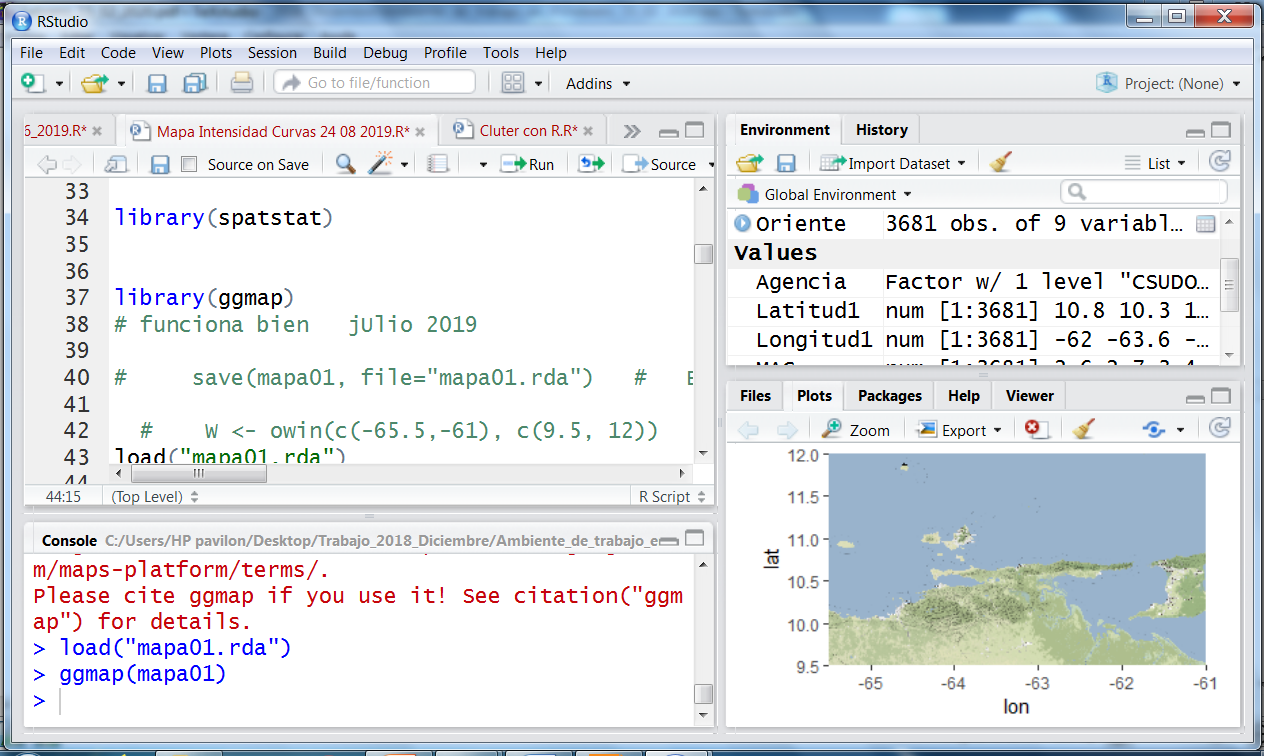
\includegraphics[width=0.7\linewidth]{../Imagenes/Rstudio2}
			\caption{Rstudio}
			\label{Rstudio}
		\end{figure}
		
		  Rstudio permite contar con una interacción más fluida con el programa R.  Básicamente se trata de una máscara para visualizar el software que tiene como principales ventajas  el orden y  la visualización de los procesos que son llevados a cabo con R, todo de manera simultánea. Rstudio presenta cuatro ventanas como se muestra en la figura \ref{Rstudio}, además de la barra de opciones en la parte superior.
			
			
		
	
		Ventana 1: es el editor de sintaxis: se trata del lugar donde editamos la sintaxis para posteriormente ejecutarla (Run).
		
		Ventana 2: es el “entorno de trabajo” del programa: en este lugar se muestra el conjunto de datos y los “objetos” (resultados, variables, gráficos, etc.) que se almacenan al ejecutar el análisis.
		
		Ventana 3: tiene varias sub pestañas: (i) la pestaña files permite ver el historial de archivos trabajados con el programa; (ii) la pestaña Plots permite visualizar los gráficos que se generen; (iii) la pestaña packages permite ver los paquetes descargados y guardados en el disco duro así como gestionar su instalación o actualización; (iv) la ventana help permite acceder al CRAN siempre que se cuente con conexión a Internet.
	
		
		Ventana 4: es la consola. Corresponde a lo que sería el software R en su versión básica. Allí el software ejecuta las operaciones realizadas desde el editor de sintaxis.\\
		
			%% que es R?studio	
			
			%  En la sección (ref{}) se muestra como se importa la data y exporta a un formato de archivo GIS o base de dato. 
			
			%  Package  RgoogleMaps September 28, 2013. Interface \\
			
				
		
			
			
			
			\section{Paquetes de R para el Análisis Espacial}{\label{R1} }
			
			
		En esta investigación el interés no es  rescribir el código de los paquetes, pues el objetivo es implementar las técnicas del análisis espacial mediante el uso de los paquetes de R, y  visualizar la data espacial en mapas obtenido de un servidor de mapas, mediante la API's  correspondiente;  en este sentido sólo se describen brevemente los paquetes empleado; sin embargo los códigos y funciones de R  necesario para llevar a cabo este trabajo se proporcionan con la finalidad de incentivar el uso de la técnicas en la investigación. A continuación exponemos brevemente el Paquete Spatstat, el más importante en esta investigación. Sin embargo, se emplean otros paquetes para visualizar la data y la intensidad del proceso en el mapa de la región en estudio, como el paquete Maptools,  Ggmap y Ggplot2.  El paquete ggmap de $R$ facilita la recuperación de mosaicos de mapas ráster de servicios de mapeo en línea populares como Google Maps y Stamen Maps y trazarlos usando el marco de ggplot2:  \\ 
			
			\textbf{Spatstat} (Spatial point pattern analysis and modelling)  es un paquete muy completo para el análisis de la data espacial, particularmente para analizar patrones puntuales espaciales, escrito por Adrian Baddeley\cite{Badbeley}   y  Rolf Turnerl. El paquete soporta la creación, manipulación y gráficos de patrones puntuales, análisis de exploratorio de la data, simulación de modelos de procesos puntuales, ajuste de modelo paramétrico, test de hipótesis, gráfico de residuos, diagnóstico de modelos. Siendo Spatstat  una de las  mayores contribuciones  disponibles  en R. Además tiene su propio dominio Web, www.spatstat.org, donde ofrece información acerca del paquete.\\   
			  
			Para el tratamiento de la data espacial, el paquete usa un objetos ppp(), que representa los patrones puntuales espaciales bidimensional. El objeto contiene las coordenadas del ppp, la intensidad,  también  incluye la región  donde los puntos de la data ha sido observada (región acotada),  llamada ventana de observación.\\
	
			
		    Más aún, aparte de los procesos y  patrones puntuales bidimensionales, spatstat también soporta patrones en tres dimensiones, patrones puntuales multidimensional espacio-tiempo,  patrones de líneas de segmentos, tessellations espaciales y conjuntos aleatorios en dos dimensiones.\\
	 
			 
			 En esta investigación se usan las funciones  F, G, K, L; funciones que se emplean para  describir la aleatoriedad espacial completa, y son descritas en la sección \ref{funciones}.   El paquete spatstat  provee las herramientas necesarias que permiten calcular tales  funciones, como objetos y algoritmo. \\
			
		
			
			
			\subsection{Código de R }{\label{codigo} }
				
				En esta sección se escribe el código empleado para calcular las funciones $ F, G, K, $ y $ L$. El código para usar visualizar la data en el mapa, la API junto con la data en estudio. Y el código para obtener la intensidad y una visualización en dos y tres dimensiones.\\
						
\textbf{La función $G$: Distancia al evento más cercano}{\label{G-codigo} }\\
			
			
		    Para el cálculo de la función $G$ se emplea el siguiente código del paquete spatstat:  	\\
				
		%	Del texto   Baddeley A.-Analysing spatial point patterns in R  y colombiano
		
			
		%	{\tiny   diminuto 
		
				{ \scriptsize  { \ttfamily  
					W <- owin(c(-65.5,-61.4), c(9.5, 12))        \#  Ventana de Observación
					
					ppp <- as.ppp( Datos , W , marks = Marcas)   \#  Patrón
					
					Reducido <- ppp[W]                         \# Datos en la región de estudio
					
				 	Oriente <-   unique(Reducido)               \#  Eliminando Datos duplicado
				 	
					r <- seq(0, sqrt( 4)/6, by = 0.0001)         \#  cambio de distancia r 
										
					spOriente <- as(Oriente, "SpatialPoints")   \#   Objeto Clase SpatialPoints
						
				    spOriente1 <- elide(spOriente, scale = TRUE, unitsq = TRUE)    \#    library(maptools)
				    				
					Oriente <- envelope(as(spOriente1, "ppp"), fun = Gest,r = r, nrank = 2, nsim = 99)  \vspace{-0,15 cm}
										
					plot(Oriente,legend=F, main= "Función G con bandas de confianza")  }}  \\
			
					
			El resultado muestra la función empírica $G(r)$  contra la función $ \hat{G}(r)$ con sus intervalos de confianza al 96\%  usando el mismo patrón de puntos en que se examina la función G.				
			La función para calcular los intervalos de confianza (envelope) es  muy flexible,  puede ser usada para calcular intervalos de Monte Carlo de cierto tipo de funciones. Básicamente, esto es por simulación aleatoria de un número de puntos del patrón, así que la función summary es calculada para todos ellos. \\
			 
				  
\textbf{La función $F$: Distancia de un punto al evento más cercano}{\label{F-codigo} }\\
				  
		 	Para el cálculo de la función $F$ se emplea el siguiente código del paquete spatstat:  \\	
					
					
				%	set.seed(30) 
				
					 	{ \scriptsize  { \ttfamily 	 
			    \#    F3 <-Fest(Oriente)
			    
				\#    plot(F3)	
															
				plot(envelope(Oriente, Fest), main= "Función F con bandas de confianza") \vspace{-0,15 cm}
											
				plot(envelope(Oriente, Fest),legend=F, main= "Función F con bandas de confianza")  }}  \\
			
				
		     	El resultado muestra la función empírica $ F$ y su intervalos de confianza asociados a 96\% .\\
				
  \textbf{La función $K$ y $L$}{\label{K-codigo}\\
   	
				
				Para el cálculo de la función $K$ y $L$ se emplea el siguiente código del paquete spatstat:  \\
				
		
			
		{ \scriptsize  { \ttfamily	
				
				K\_Oriente <- envelope(as(spOriente1, "ppp"), fun = Kest,r = r, nrank = 2, nsim = 99)
				
				plot(K\_Oriente, legend=T,  main= "Función K con bandas de confianza")
				
				L1 <- envelope(Oriente, Kest) 
				
				plot(L1, . - pi*r\^{}\{2\} \~{} r, legend=F,  main="Función L")  \vspace{-0,15 cm} 
				
				% problemas con el simbolo ^ y ~     
				
				plot(L1, sqrt(./pi) \~{} r, main="Función L")  }}  \\
			
	Los  valores de la función K para un PPHP es $K(s)=\pi s^2$.   Para comparar la estimación de la función $K(s)$ con el valor teórico, usualmente se  asume que esas interacciones ocurren en pequeñas escales. Así el interés es relativamente en valores pequeños de s. 
	
	 Valores de $K(s)$ mayores que $\pi s^{2}$ son característica de proceso con clúster, mientras que valores menores que ese valor se encuentran cuando existe regularidad competición entre los eventos (patrón regular).\\
				
				
		
			
   \textbf{Estimation de intensidad}{\label{Intensidad_Codigo}\\
				
					

   \textbf{Intensidad uniforme}\\
	
	
	Si el  proceso  puntual es  Homogéneo la estimación de la  intensidad  está dada por 
	
	\[ \: \widehat{\lambda} = \frac{n}{|A|} \] un estimador insesgado de la intensidad homogénea  \ref{Intensidad_Homogenea}.\\ 

Para calcular el estimador de la  intensidad basta con usar el resumen del objeto ppp (summary.ppp), como se indica a continuación:\\


	{ \scriptsize  { \ttfamily	

		 
  summary(Oriente)  
  
  Intensidad  <- summary(Oriente)\$intensity \vspace{-0,15 cm} 
  
  Intensidad }}  	\\
  
  
  El resultado es numérico,  indicando el número  promedio de puntos por unidad cuadrada.\\
  
 
	
	%%%%%%%%%%%%%%%%%%%%%%%%%%%%%%%%%%%%%    Para   Intensidad  no homogeneo       %%%%%%%%%%%%%%%%%%%%%%%%%%%%%%%%%%%%%%%%%
						

  \textbf{Intensidad no homogénea}{\label{Intensidad_no_homogenes}\\
	
	 En el caso de la intensidad es no homogénea, la función o medidad de intensidad  puede ser calculada por la técnicas del cuadrante o kernel. \\ 
	 
  \textbf{Técnica de los Cuadrantes}{\label{TCuadrantes}\\
	 		
	 En el caso de usar la técnica del cuadrante, el área de estudio o ventana de observación es dividida en subregiones o cuadrantes $ B_{1}, \dots, B_{m} $ de igual área; y cuenta el número de puntos que caen en cada cuadrante $ ( n_{j}  = E( X_{B_{j}} ),$ 	  para cada  $ j = 1, \dots, m ).$   Estos  son  estimadores insesgados correspondientes a la medidad de intensidad en $B_{j}.$ 	Para calcular la intensidad por el método de los cuadrantes se aplica el comando quadratcount() del paquete spatstat  al objeto ppp, como se muestra en el siguiente  código \\	
	
	 %  tomado del texto     {\footnote{Adrian Baddeley, 2010, Analysing spatial point patterns in R}
	
	{ \scriptsize  { \ttfamily	
		Oriente
				
	Cuadrantes <- quadratcount(Oriente, nx = 3, ny = 3)  
	
	Cuadrantes
		
	plot(Oriente, cex = 0.5, pch = 20) \vspace{-0,15 cm}
	
	plot(Cuadrantes, add = TRUE, cex = 1.5) }}\\   

	El resultado es un objecto perteneciente a la clase  “quadratcount'',  indicando la distribución de puntos en los cuadrantes, y un gráfico de los cuadrantes con el número de puntos en cada uno.\\ 
	
		{ \scriptsize  { \ttfamily	
				 
	 Cuadrantes <- quadrat.test(Oriente, nx=3, ny=3)   % ## Babdeley pag 89 y Colombiano   
	 
                                                  %  ##  homogeneous Poisson process (CSR)
     plot(Oriente)                                %  ## hacer un cambio de color de letras
     
                                                  %  ##  o color de puntos
     plot(Qtest, add=TRUE)

     Qtest

     Qtest\$p.value    \vspace{-0,15 cm}     
                                                                                  
     Qtest\$statistic                      }}\\


Además, ofrece un test de aleatoriedad que se puede visualizar en el gráfico de los cuadrantes, con el conteo y el valor de Chi-cuadrado.\\



     \textbf{Método del Kernel para estimar la intensidad }{\label{I4-codigo}\\
      
      El paquete spatstat calcula la estimación de densidad del Kernel (o intensidad)  usando un núcleo Gaussian mediante la función density() aplicada al objeto  ppp(), como se muestra a continuación \\
 
 
  	
  \textbf{Código Intensidad}\\
  
  { \scriptsize  { \ttfamily  	
  		
  		Oriente
  		
  		Intensidad <- density(Oriente, sigma = 0.15)  \#  sigma es ancho de la ventana 
  		
  		plot(Intensidad, axes = T, cex = 0.5, col= rev(heat.colors(100)), 
  		
  		font = 0.5, xlab = "Lonitud",  ylab = "Latitud", main= “  ")  \vspace{-0.15cm}
  		
  		title(main =list( “Estimación de Intensidad", cex = 1.5, font = 4)) 	}}\\
  


	
		El resultado obtenido por la función density.ppp con el comando density(), es una clase tipo imagen (objecto de clase     "\! im"); el mismo puede presentarse en resumen (summary),  en  gráficos (plot), en gráfico de contorno (contour) y en un gráfico en tres dimensiones,  como se muestra acontinuación:  \\
		
		% tomado de pag 80  	{\footnote{Adrian Baddeley, 2010, Analysing spatial point patterns in R}
		
		    
		
		
		
			
	  % 	Kernel density (or intensity) estimation using an isotropic Gaussian kernel is implemented in spatstat by the function density.ppp, a method for the generic command density	
	
	
	   	
	   \textbf{Código para contornos}\\
	   
	   { \scriptsize  { \ttfamily 
	   		
	   		Intensidad <- density(Oriente, sigma = 0.20)  \#  sigma es ancho de la ventana
	   		
	   		contour(Intensidad, axes = T,  col=  “red", font =1.5, cex = 1.5,
	   		
	   		xlab = "Lonitud", ylab = "Latitud", main= “  ")  
	   		
	   		plot(Oriente, add = TRUE , pch= 20, size = 0.3)  \# Agregando puntos \vspace{-0.15cm}
	   		
	   		title(main =list("Gráfico de contornos", cex = 1.5,  font = 4))  }}\\
	   
	   
	
	\textbf{Método gráfico para visualizar la intensidad en tres dimensiones}{\label{Pesrs}\\
		
		Un método interesante para visualizar la intensidad de un proceso espacial en tres dimensiones se obtiene con ayuda del comando { \ttfamily persp()}, el código se expone a continuación:\\
		
		{ \scriptsize { \ttfamily 
				
				
				Intensidad <- density(Oriente,sigma = 0.20)  
				
				persp(Intensidad, phi = 25, theta =45, d = 5, shade =0.01, axes = T, cex = 0.5, 
				
				font = 0.5, expand = 0.0005, col="blue", xlab = "Longitud", ylab = "Latitud", \vspace{-0,15 cm}  
				
				zlab = “Intensidad", main= “ Estimación de intensidad")  	} }\\
		
		
		
		
	     	

 
		
		
		%%%%%%%%%%%%%%%%%%%%%%%%%%%%%%%%%%%%%   Fin  Intensidad  no homogeneo       %%%%%%%%%%%%%%%%%%%%%%%%%%%%%%%%%%%%%%%%%
		
		\textbf{Método alternativo }{\label{Pesrs}\\
				
		Alternativamente, el paquete  spatstat ofrece para calcular la estimación de la  intensidad mediante la técnica de paramétro adaptativa para en ancho de banda $h.$	\\	
		
	
		{ \scriptsize  { \ttfamily   
				
				Adaptativo <- adaptive.density(Oriente, f = 0.01, nrep = 10)  	
			
				plot(Adaptativo, main = “Adaptive intensity")	\vspace{-0.15cm}   
				
				plot(Oriente, add =TRUE ,cex = 0.5, size = 0.001)         }}   \\
			  
			El resultado es también una imagen (Objeto de clase "\! im").\\
			
		
	
    %  	Babdeley pag 89 {\footnote{Adrian Baddeley, 2010, Analysing spatial point patterns in R}
		
				
			           
			
		
		
		
  

					
				
				\subsection{Código de R para obtener mapas}{\label{R1} }
				
		Para obtener el mapa de la zona en estudio se emplea la libreria o paquete ggmap ({{\ttfamily 
		library(ggmap)}})  de  $R$  y  el  código   {{\ttfamily get\_stamenmap()}}.\\	
		
		
		\textbf{Mapas de la zona oriental de Venezuela con la data}{\label{M-codigo}\\
			
				   
			
			{ \scriptsize  { \ttfamily 
				   library(ggmap) 
				   	
				   Zona <- c(bottom  = 9.7, top = 11.3,left  = -65, right = -61)
				   	
				   map <- get\_stamenmap(Zona, zoom = 10, maptype = "terrain")
				   	
				   W <- owin(c(-65,-61), c(9.8, 11.2))  \#  Ventana de observación
				   	
				   ppp <- as.ppp( Datos , W , marks = Marcas)   \# Patrón
					
				   Reducido <- ppp[W]	 \# patrón reducido por vententana de observacón			
				   				    
				   Redu <-  data.frame(Reducido\$x, Reducido\$y) 
				   
				   ggmap(map) +                                    \vspace{-0,15 cm} 
					
				   geom\_point(data = Redu, mapping = aes(x = Reducido\$x, y = Reducido\$y), size = 0.001 )   }} \\
			
				
			
		
			
		\textbf{Mapas de la zona con mayor concentración de eventos sísmicos}{\label{M-codigo}\\
			
				
			{ \scriptsize  { \ttfamily 
				
		
		            
		             
		W2 <- owin(c(-63.5,-62), c(10.2, 11))
		
		Zona\_R <- c(bottom  = 10.2, top = 11, left  = -63.5, right = -62)
		
		Region <- get$\_$stamenmap(Zona\_R, zoom = 10, maptype = "terrain")
			
	
				
		Reducido$\_$g <- ppp[W2]
		
		Data\_R <- data.frame(Longitud=Reducido$\_$g\$x,Latitud=Reducido$\_$g\$y)  
		
		ggmap(Region) +           \vspace{-0,15 cm}
		
		geom$\_$point(data = Data\_R, mapping = 
		aes(x = Longitud, y = Latitud), size= 0.01)     }}	\\
			
			
			
				
		
		\textbf{Profundidad vs Magnitud de los sísmos}{\label{M-codigo}\\
		
		
				
					
			{ \scriptsize  { \ttfamily 
					
				library(MASS)
				
				ggplot(Redu, aes(x = Magnitud,y = Profundidad)) + 	\vspace{-0,15 cm} 
				
				geom$\_$point(col = "blue") + 	geom$\_$density2d(col = "White")       	}}\\
			    
			    
			    \textbf{Código para graficar de la Magnitud por categoría de acuerdo a la escala de Richter}{\label{M-codigo}\\
			 
			 
			 	{ \scriptsize  { \ttfamily 
			 		
			 		Profundidad<-Reducido\$marks\$PROFUN\_KM 
			 		
			 		Magnitud <- Reducido\$marks\$MAG
			 		
			 		long <- Reducido\$x; lat <- Reducido\$y
			 		
			 		Redu\_Categ <-  data.frame(long, lat,Magnitud,Profundidad)     
			 		
			 		is.data.frame(Redu\_Categ)
			 		
			 		Mayor <- Inf          %  \#    ≥    ≤
			 		
			 		Redu\_Categ[,"Mag\_C"] <- cut(Redu\_Categ\$Magnitud,
			 		
			 		breaks = c(0,   3.51, 5.41, 6, 7, Mayor),
			 		
			 		labels = c("0.1 <Mag< 3.5","3.5< Mag <5.4", "5.4 < Mag< 6 ","6 < Mag< 7" , "Mag > 7") )
			 		
			 		%	head(Redu\_Categ)
			 		
			 		data1<- Redu\_Categ
			 		
			 		%	Redu\_Categ
			 		
			 		%	library(ggmap)
			 		
			 		%	summary(Redu\_Categ)
			 		
			 		\#	load("mapa01.rda"); 	map <- ggmap(mapa01)
			 		
			 		cex=c( 0.4, 0.6, 1.5, 2.5, 3 ) 
			 		
			 		col = c( “grey",“green",“blue",“orange",“red")
			 		
			 		Mag\_C <- data1\$Mag\_C  }}
			 
			 
			 
			 
			 
			 	
			 	{ \scriptsize  { \ttfamily    
			    
			    
			    map + geom$\_$point(data = data1,  aes(x = long, y = lat, fill = factor (Mag$\_$C) ),
			    
			     pch = 21,  cex= 0.6*MAG$\_$Redu ,  alpha = 0.7) + 
			     
			    scale$\_$fill$\_$manual(values = col, name = "Magnitud")+ 
			    
			    scale$\_$color$\_$manual(values = col)+
			    
			    theme( 
			    legend.position = c(0.86,0.01), legend.justification = c(0, 0),
			    
			    legend.background = element$\_$rect(colour = F, fill = "white"),
			    
			    legend.key = element$\_$rect (fill = F, colour = F),   \vspace{-0,15 cm} 
			    
			    panel.grid.major = element$\_$blank (),  panel.grid.minor = element$\_$blank() )           
		                           }}  \\
			    
			    
			    		
			  \textbf{Código para  gráficar la profundidad por categoría de acuerdo a cuartiles y profundidad}{\label{M-codigo}\\			 				
			  
			  
			   { \scriptsize  { \ttfamily  		
			  		
			  
			  
			  
			  Profundidad<-Reducido\$marks\$PROFUN\_KM
			   
			  Magnitud <- Reducido\$marks\$MAG
			  
			  long <- Reducido\$x
			  
			  lat <- Reducido\$y
			  
			  Redu\_Categ2 <-  data.frame(long, lat,Magnitud,Profundidad)  
			         
			  is.data.frame(Redu\_Categ2)
			  
			  Mayor <- Inf
			  
			  Redu\_Categ2[,"Prof\_C"] <- cut(Redu\_Categ2\$Profundidad,
			  
			   breaks = c(-0.01, 4,12,  37, 70, Mayor),
			   
			   labels = c("0.1 <Prof < 4","4 < Prof < 12",  "12 < Prof < 37 ","37 < Prof < 70 ", "Prof > 70" ) )
			 % head(Redu\_Categ2)
			 
			  data2<- Redu\_Categ2
			  
			  col2 = c(“grey", “green", “blue", “orange", “red")
			  
			 % library(ggmap)
			 % load("mapa.rda")
			 % ggmap(mapa)
			 % map <- ggmap(mapa)
			 
			  Prof\_C <- data2\$Prof\_C    }}
			  
			  
			  
			  
			  
			  
			  
			    { \scriptsize  { \ttfamily  		
			    
			    
			    map + geom$\_$point(data = data2,  aes(x = long, y = lat, fill = factor(Prof$\_$C) ),
			    
			     pch = 21,  cex  = 1.2*PROFUN$\_$KM$\_$Redu/40 ,  alpha = 0.5) +
			     
			    scale$\_$fill$\_$manual(values = col2, name = "Profundidad") +
			    
			     scale$\_$color$\_$manual(values = col2)+
			    
			    theme( legend.position = c(0.86,0.01),  legend.justification = c(0, 0),
			    
			    legend.background = element$\_$rect(colour = F, fill = "white"),
			    
			    legend.key = element$\_$rect(fill = F, colour = F),    \vspace{-0,15 cm} 
			    
			    panel.grid.major = element$\_$blank(), panel.grid.minor = element$\_$blank() )    }}  \\
			     
			     
			
		 
			     %	Voy en pagina 194 de que libro \\
				
			    %   Applied Spatial Data Analysis with R  , Roger S. Bivand • Edzer J. Pebesma y
			    %                               Virgilio Gómez-Rubio 
			                      
			            
			            
			            
			 
			  		
			\textbf{Código para presentar la intensidad sobre el mapa}{\label{M-codigo}\\			 				
				
				{ \scriptsize  { \ttfamily            
			 
			 
		%	 get$\_$stamenmap     \# library(ggmap)
			 
			 ggmap(map) +  
			 
			 stat$\_$density2d( aes(x = Reducido\$x, y = Reducido\$y,  alpha = 0.01),
			 
			 size = 0.001, bins = 15, data = Redu, geom = "density$\_$2d", color="\#FFFFFF") + 
			 
			 stat$\_$density2d( aes(x = Reducido\$x, y = Reducido\$y,
			  
			 fill = ..level.., alpha = 0.001),
			 
			 size = 0.009, bins = 10, data = Redu, geom = "polygon" ) +
			 
			 scale$\_$fill$\_$continuous(low = “\#FFFF00", high =  “red", space = "Lab", name = "Bajo")  + \vspace{-0.15cm}
			 
			 scale$\_$colour$\_$discrete(guide = FALSE) +  theme(legend.position="bottom")   }} \\
			            
			 	\textbf{Código para  gráficar contornos en el mapa}{\label{M-codigo}\\			 				
			 	
			 	{ \scriptsize  { \ttfamily   	
		
	    	qmplot(x = Reducido.x, y = Reducido.y, data = Redu,	
	    	
	    	maptype = "terrain", bins = 15,   geom = "density2d", color = I(“red")) + \vspace{-0.15cm}
	    	
	    	
		       theme(legend.position="bottom")     }}	\\ 			
			 	
			 				
			
	%	\end{document}  “ 
	

Con esta exposición culminamos esta sección correspondiente a describir los paquetes y código del software r usados en la investigación. En el próximo capítulo  se analizan los cálculos resultados de la aplicación de las técnicas descritas.  
             
				
  \chapter{Análisis y resultados}
				
		
		\section*{Introducción}
		
		En este capítulo, se analiza la data correspondiente a los eventos sísmicos en la zona oriental de Venezuela, mediante las técnicas de estadística espacial y los sistemas de información geográficos (SIG); específicamente el software  R,  con  paquetes para estadística espacial, y las API's,  que permiten el tratamiento geoestadístico aplicado a base de datos georeferenciados, facilitando la manipulación y posibilidad de visualizar gráficamente el comportamiento del fenómeno, tanto en espacio como en el tiempo. Sin embargo, esta investigación consiste sólo en describir  los patrones puntuales del proceso; empleando para éste fin, el paquetes Spatstat del software R, y los paquetes que  permiten tratar la información como en los sistemas de información geográfico, así como la visualización de  la información en el mapa, y análisis de patrones puntuales. \\
		
		Además, se espera dar a conocer de manera sencilla y práctica el poder de las técnicas de estadística espacial del software R combinado con  API's, y  los SIG, de tal manera que motive el uso y la  aplicación de estas técnicas y herramientas en las diferentes áreas. \\
		
		%(en futuros estudios elaboración de mapas de amenaza y peligro y que permitirá por consiguiente la toma de decisiones en multitud de campos, particularmente en materia de riesgos de fenómenos naturales).\\
		
		
		Para desarrollar el análisis exploratorio de datos espaciales, como primer paso se presenta el mapa de los eventos sismos, que consiste simplemente en ubicar los puntos (epicentro del sismo) en el mapa de la zona en estudio;  seguidamente se calculan los estadísticos descriptivos,  método de los cuadrantes, las funciones $F, G, K, L$.  Se calcula la intensidad con método del kernel, presentándose sobre el área de estudio como suavizado de kernel, en curvas de nivel o contornos y en tres dimensiones.\\
		
		Finalmente se presenta sobre el mapa obtenido del servidor Stamen Maps  la intensidad calculada también con método del kernel y curvas de nivel o contornos.\\
							
	
			 
			\section{Análisis descriptivo}
				
				
		La figura \ref{Mapa} muestra el mapa los eventos sísmicos en la zona Nor-oriental de Venezuela, durante el periodo  09/01/1995 al  02/10/2018. En el mismo se puede apreciar concentraciones ubicadas entre la Península de Araya, municipio Cruz Salmerón Acosta (Araya)  y la cuidad de Cumaná;  una concentración aunque pequeña se muestra en  la zona que comprende la parte Este del golfo de Cariaco, específicamente en los municipio Ribero (Cariaco), y el municipio Mejía (San Antonio del Golfo);   se observa una alta concentración  en la zona central del estado sucre, que se ubica entre los municipios Bermúdez (Carúpano),  Andrés Eloy Blanco (Casanay),  Andrés Mata (San José de Aerocuar), Benítez (El Pilar) y Libertador (Tunapuy);  y una gran concentración aunque un poco dispersa por el mar Caribe, al norte de la península de Paria.
				
				\begin{figure}[h!]\label{Sismo}
					\centering
					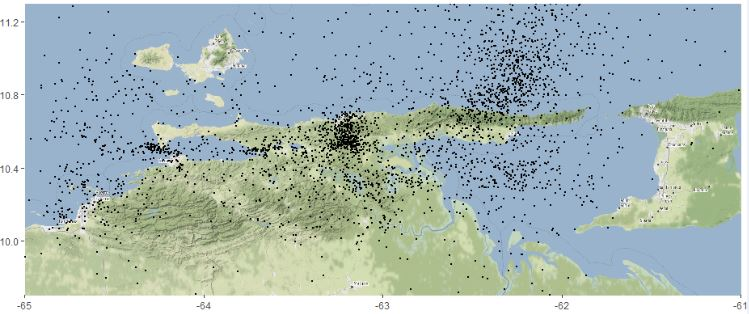
\includegraphics[scale=0.85]{../Imagenes/MOriente1}       %950JPG
					\caption{Mapa de los eventos sísmicos en la zona Oriental de Venezuela, periodo 1995 a 2018}
					\label{Mapa}
				\end{figure}
				
		Evaluando la zona geográfica (latitud y longitud) donde suelen tener lugar los movimientos sísmicos, se presentan ambas magnitudes por separado en el gráfico \ref{Lat_y_Long}.  En el mismo podemos ver como el mayor número de sismos  se concentran entre las longitud -63.5  y -62, con una media igual a -63.06, en cuanto a latitud se concentran en el rango de  10.2 a 11.2, con una media igua a	10.630.	
		
		\begin{figure}[h!]
			\centering
			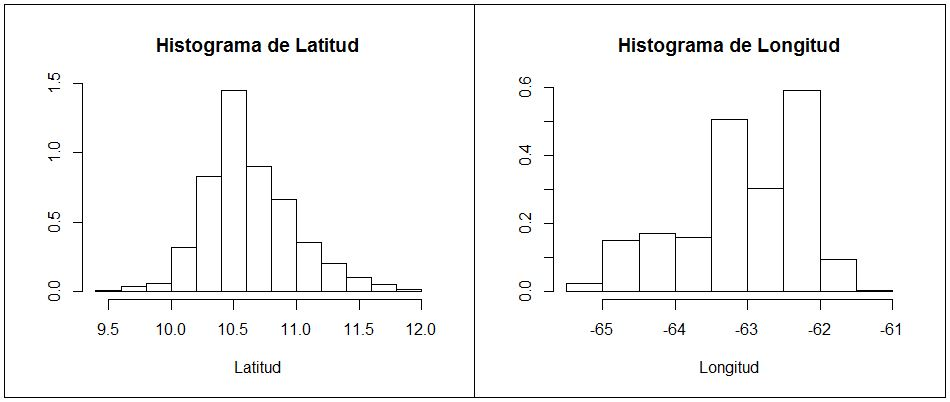
\includegraphics[width=0.8\linewidth, height=0.2\textheight]{../Imagenes/Lat_y_Lon}
			\caption{ Latitud y Longitud }
			\label{Lat_y_Long}
		\end{figure}
		
	
	En la zona con mayor concentración de eventos sísmicos (figura  \ref{Region})  se encuentran los pueblos de Carúpano, Cariaco, Casanay, San José de Aerocuar,  Tunapuy, Río Caribe, Irapa, Yaguaraparo, Güiria; un alto porcentaje de la población del estado sucre, que corresponde a 10 municipios de los 15 en total del estado Sucre.\\    %   Guaria
		
		
		\begin{figure}[h!]
			\centering
			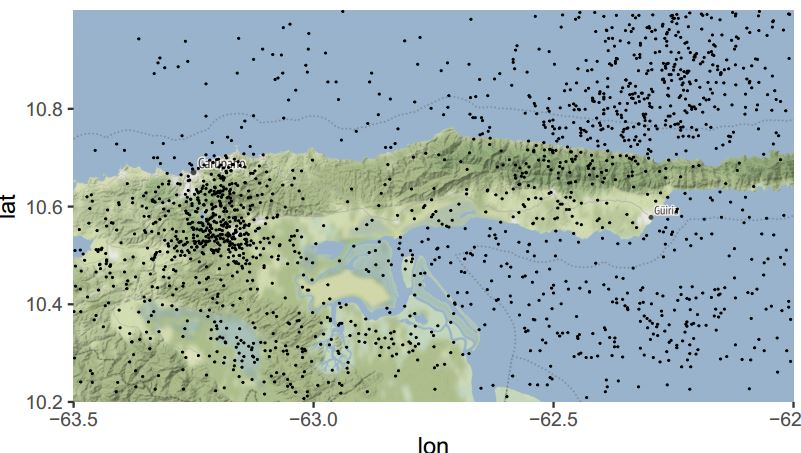
\includegraphics[scale=0.4]{../Imagenes/Region05}
			\caption{Zona geográfica con mayor concentración eventos sísmicos}
			\label{Region}
		\end{figure}
		
				
		
		\subsection{Magnitud y Profundidad}   	% percentil 0.79842375 en 50 Km	

		En el cuadro \ref{DescriptivoMP}  se presenta el resumen estadístico de la  Magnitud  (medida en escala de Richter) y Profundidad  de los sismos. En el mismo se observa  la magnitud  variando  en un rango  0.1  a 7.3,  con una media igual a 2.7,  presentando una  distribución  simétrica como se observa en la figura \ref{HisProfMag}. Concentrando el 83\% de los datos en el rango magnitud: 2 a 4 (percentil 14 y 97, con magnitud 2, 4 respectivamente). 			
			\begin{table}[h!] 
				\centering
				\caption{Estadísticos descriptivos}\vspace{-0.2cm}
				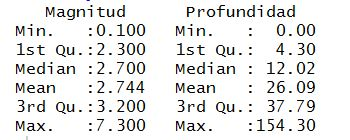
\includegraphics[scale=0.85]{../Imagenes/DescriptivoMP}
				\label{DescriptivoMP}
			\end{table} 		En cuanto a la  profundidad esta presenta con una distribución irregular (asimétrica con sesgo hacia la derecha, ver en figura \ref{HisProfMag}), con  una media igual a  26.09 Km, alcanzando aproximadamente el 80\%  de datos  en  50 Km (percentil 80.0 , 52.08 Km).	El 20 \% restante de los datos por encima de 50 Km forman una especie de grupo con magnitud en un rango de 2 a 4, como se observa en el histograma \ref{HisProfMag} y se muestra gráfico \ref{Prof_vs_Mag}.
			\begin{figure}[h!]
			\centering
			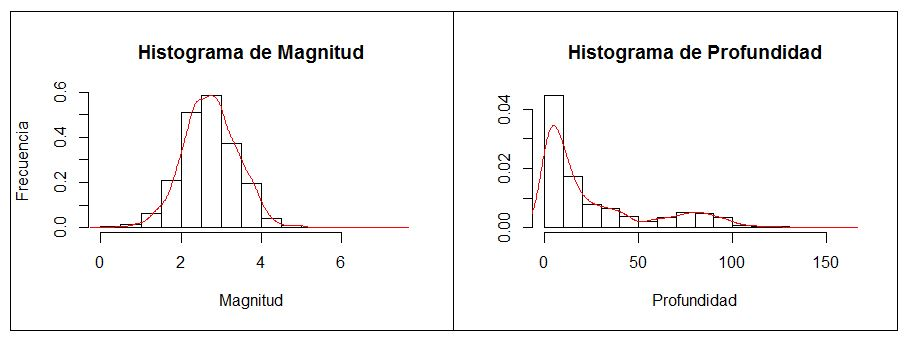
\includegraphics[width=0.8\linewidth, height=0.2\textheight]{../Imagenes/His_Prof_Mag}
			\caption{Histograma de Magnitud y Profundidad}
			\label{HisProfMag}
		\end{figure}	
		
	
	
		
		
				
		\begin{figure}[h!]
			\centering
			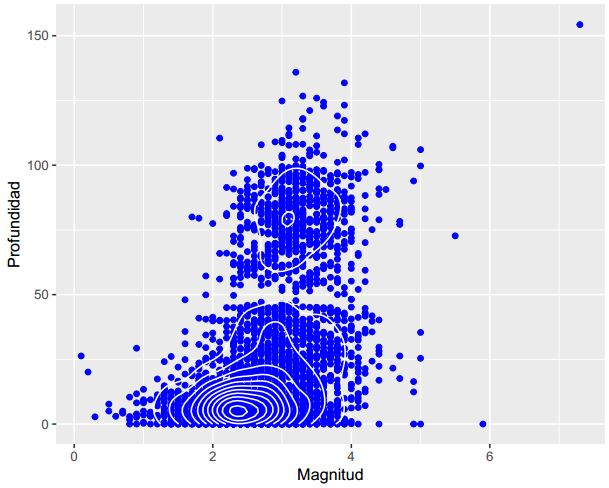
\includegraphics[width=0.6\linewidth, height=0.3\textheight]{../Imagenes/Prof_vs_Mag}
			\caption{Profundidad vs Magnitud}
			\label{Prof_vs_Mag}
		\end{figure}
		
	En la figura \ref{Prof_vs_Mag} se presenta la Magnitud vs la Profundidad, se puede observar la gran liberación de energía  en eventos sísmicos con magnitud menor a 4 y profundidad menor a 50 Km,  y se refleja un grupo en un rango que va de 50 a 100 Km de profundidad, con magnitud en un rango: 2.5 a 4. Además, se observa una tendencia en cuanto a mayor magnitud, mayor profundidad, sin embargo las magnitudes grandes son poco frecuentes, posiblemente debido a la gran liberación de energía con sismos de magnitudes bajas (menor a 3.5, aproximadamente 85\% de los sismos), ayudando a evitar que se acumule y se convierta en un gran sismo con consecuencias catastróficas. \\
	
	
%		% percentil 0.79842375 en 50 Km	


El cuadro \ref{Efectos}  muestra los efectos que generan los sismos de acuerdo con la escala de  magnitudes de Richter.  Para los sismos con magnitud menor 		
\begin{table}[h!] 
	\centering
	\caption{ {Escala de Magnitudes de Richter y Efectos del sismo}} \vspace{-0.2cm}
	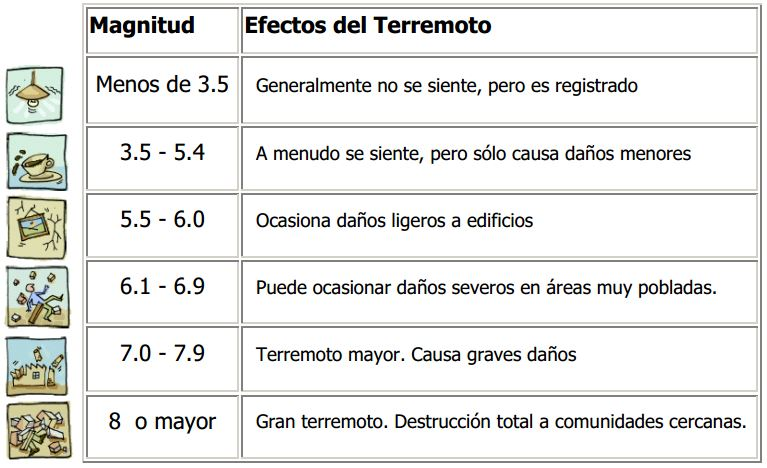
\includegraphics[scale=0.6]{../Imagenes/Efectos}\vspace{-0.1cm}
    \caption*{\ttfamily (http://www.angelfire.com/nt/terremotos)}
	\label{Efectos}
\end{table} a 3.5, los efectos generalmente no se sienten; mientras que  para magnitudes entre 3.5 y 5.4 la población los siente, pero los  daños son menores. El catálogo de sismicidad analizado en esta investigación  presenta el 95\% de los sismos con magnitud menor a 5.4 (percentil 95\%, 5.4); mientras que el 5\% restante (mayor a 5.4) alcanza una magnitud máxima de  7.3; además, el porcentaje de sismos con magnitud mayor 6.1  es bajo (percentil 99.9745\% , 6.122257 ).\\

%  \caption[Escala de Magnitudes de Richter y Efectos del sismo]{Escala de Magnitudes de Richter y Efectos del sismo\\
%	{\scriptsize { \ttfamily (http://www.angelfire.com/nt/terremotos)} }  }



	%     \includegraphics[scale=0.7]{../Imagenes/K015jpeg}  con ancho de banda 0.15
	
%	{ \scriptsize  { \ttfamily      }  }

%       \begin{changemargin}{5cm}{15cm}  \end{changemargin}



\textbf{Gráfico de Magnitudes de Richter y Profundidad}{\label{Magnitud_G}\\	
   
 
El mapeo para la magnitud y la profundidad de los sismos se organizó en categorías para visualizarla en el mapa de la zona en estudio. En las  figuras  \ref{Magnitud} y \ref{Profundidad} se muestra los resultados de Magnitud y Profundidad respectivamente.  La magnitud categorizada de acuerdo con los efectos producidos por la magnitud, y la profundidad se categorizó tomando en cuenta los cuartiles y valores muy altos en la data.
La distribución de la magnitud para valores menores o igual a 3.5 (color gris) se observa por todo el área en estudio, con mayores concentraciones en tres  regiones; una aunque pequeña se observa en la región  comprendida entre Cumaná y Punta Araya, otra se ubica en la
\begin{figure}[h!]
	\centering
	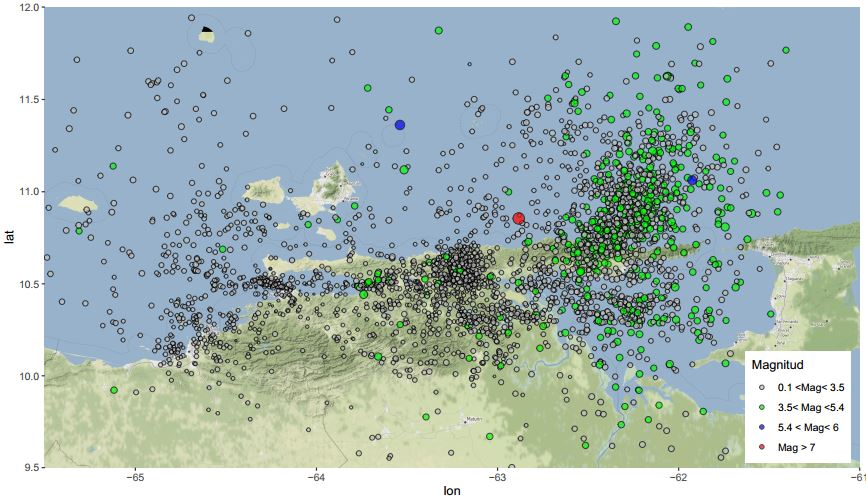
\includegraphics[scale=0.55]{../Imagenes/Magnitud01}
	\caption{Magnitud en escala de Richter}
	\label{Magnitud}
\end{figure} parte  central del estado Sucre, específicamente en la zona donde se encuentran los municipios Bermúdez (Carúpano),  Andrés Eloy Blanco (Casanay),  Andrés Mata (San José de Aerocuar), Benítez (El Pilar) y Libertador (Tunapuy);  y una gran concentración sobre el mar Caribe, al norte de la península de Paria. Mientras que la distribución de la magnitud categoría 3.5-5.4 (color verde), se observa con mayor incidencia al oriente, específicamente entre golfo de Paria y Mar caribe, con los municipios Valdez (Güiria) y  Mariño (Irapa) en medio. Las magnitudes mayores a 5.4 se observan solo tres eventos, ubicándose al nor-oriente de la región en el mar caribe,  dos con magnitud de la categoría 5.4-6 (color azul), y uno con magnitud mayor a 7 (color rojo); en la categoría correspondiente a 6-7, no se observan eventos sísmicos.  El resumen estadístico se presenta en el cuadro \ref{resumen_M}.
	\begin{table}[h!]   
		\centering
		\caption{{Resumen estadístico }}\vspace{-0.4cm}
		\caption*{{de la magnitud, y profundidad por categorías}}\vspace{-0.2cm}
		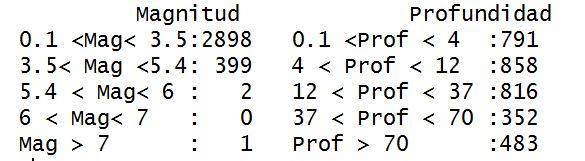
\includegraphics[scale=0.6]{../Imagenes/Resumen}      %950JPG
		\label{resumen_M}  
    \end{table}	

La distribución de los eventos sísmicos de acuerdo con la profundidad se muestran en la figura \ref{Profundidad},  con respecto a la categoría  con valores menor igual a 12 kilómetros (color gris y azul), se observa una concentración entre el sector denominado Punta Araya y la ciudad de Cumaná; una pequeña en la zona Muelle Cariaco y Cariaco;  y otra con mayor concentración al centro del estado Sucre, específicamente en la zona donde se encuentran los municipios Bermúdez (Carúpano),  Andrés Eloy Blanco (Casanay),  Andrés Mata (San José de Aerocuar), Benítez (El Pilar) y Libertador (Tunapuy). La categoría correspondiente a 12- 37 kilómetros (color azul), se observa por todo la zona en estudio, con mayor ocurrencia en la 
	\begin{figure}[h!]
		\centering
		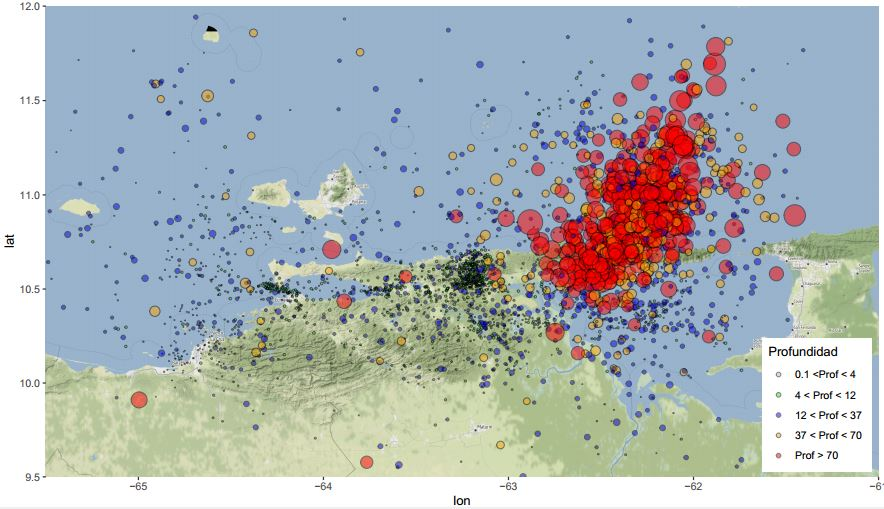
\includegraphics[scale=0.55]{../Imagenes/Profundidad10h}
		\caption{Profundidad de sismo en Km.}
		\label{Profundidad}
	\end{figure}
línea central de este a oeste (10.5 latitud), con una concentración en la zona central del estado, en la zona donde se encuentran los municipios Bermúdez (Carúpano),  Andrés Eloy Blanco (Casanay),  Andrés Mata (San José de Aerocuar), Benítez (El Pilar) y Libertador (Tunapuy). Las categorías correspondientes a 37-70 (color dorado) y mayor a 70 kilómetros (color rojo) se observa la mayor incidencia al nor-oriente de la zona en estudio, entre golfo de Paria y Mar caribe, en medio de esta región se encuentran los municipios Valdez (Güiria) y Mariño (Irapa). \\ 
  
En general, se observa claramente gran concentración de eventos sísmicos con mayor profundidad y magnitud en la zona nor-oriental de la región en estudio,  específicamente entre el golfo de Paria y mar Caribe,  en medio de esta zona de gran intensidad sísmica, se encuentran los municipios Valdez (Güiria),  y Mariño (Irapa). Mientras que las concentraciones  al centro del estado Sucre se observan con magnitud baja, menor a 3.5  y profundidad menor a 37 kilómetros.

  
%		Para el análisis espacial y temporal del catálogo de sismicidad se utiliza el software R (2.10.1).
%   	Paquete Spatstat (versión 1.18-1)
%	   Paquete Maptools (versión 0.7-34)
	
	
	
	
		
    	%   	Geographical Resources Analysis Support 			System (GRASS) de 	Roger
    	%	Packages for the Analysis of Spatial Point Patterns           roger pag 174
		
		%	  Kernel density (or intensity) estimation using an isotropic Gaussian kernel 
		%	  is implemented in spatstat by the function density.ppp, a method for the 
		%	  generic command density.      
		
		
		
		
		
	
				
				\section{Análisis del proceso puntual}{\label{Puntuales} }
				
	%    Applied Spatial Data Analysis with R  Roger muy completo  y mejor el de Baddeley 
	%  This can be analysed as a point process in space-time (where space is the two-dimensional    plane or the Earth’s surface). If the occurrence times are ignored, it becomes a spatial point   process.                                
			   
			   
	 En esta sección se analiza la aleatoriedad del patrón de puntos espaciales, es importante señalar que la hipótesis nula se refiere a un proceso puntual  homogéneo de Poisson, aleatoriedad espacial completa (AEC); en este sentido se aplica en primer lugar el método de los cuadrados, método que emplea el estadístico del chi-cuadrado, y luego se sigue con los índices o estadísticos basados en las distancia, y se obtienen algunas conclusiones.
			   
				\subsection{Método de los cuadrantes}\label{cuadrante}		
					
		En la siguiente figura \ref{cuadrantes} se presenta el patrón de puntos en la zona de estudio seleccionada como ventana de observación, definida por un rectángulo  entre las coordenadas de longitud -65.5 y -61.4 y latitud 9.5 y  12. Esta región se divide en nueve zonas. En el mismo se observa el número de puntos en cada cuadrante, el valor esperado y desviación  o residuos de Pearson. 		
		\begin{table}[h!]
		\centering
		\caption{ {Resultado del estadístico de prueba\\ Chi-cuadrado} }\vspace{-0.4cm}
		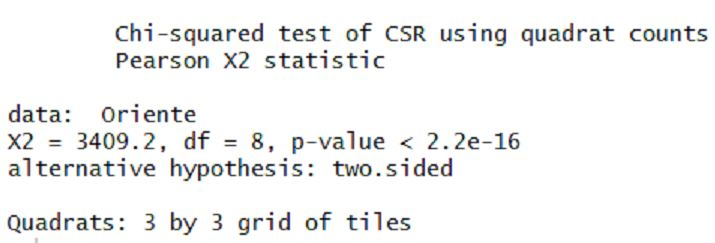
\includegraphics[width=0.6\linewidth]{../Imagenes/Qestadistico1}		
		\label{Qestadístico}
	   \end{table}
		El cuadro \ref{Qestadístico} corresponde al resultado de la prueba de aleatoriedad del método del los cuadrantes (obtenido con el comando  {\ttfamily  quadrat.test()}), en el se observa el valor del estadístico de prueba de la Chi-cuadrado  $ x^{2}_{8} =  3409.20,$  (valor de $  x^{2}_{8; 0.98} = 0,665314093$ )  con un  y el P valor muy bajo ($p-value < 2.2e-16 $); con este resultado claramente se rechaza la hipótesis de aleatoriedad espacial.  
		 \vspace{-0,85 cm}			
			\begin{figure}[h!]
			\centering
			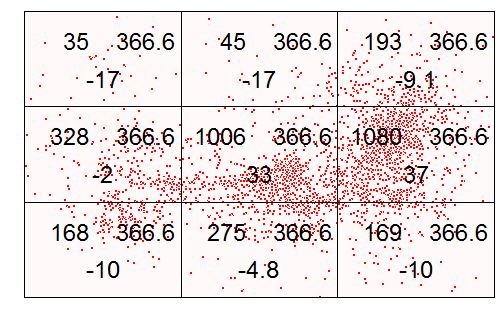
\includegraphics[width=0.6\linewidth]{../Imagenes/Cuadrantes}
			\caption{Prueba de aleatoriedad \\ Método de los cuadrantes}	
			\label{cuadrantes}			
		\end{figure}
		
		
		
		
			\subsection{Métodos basados en la distancia}\label{distancia}		
			
En esta sección se calculan los estadísticos basados en el método de la distancia, en este caso se estudian las funciones $ G, F, K, $ y $L$. Para el cálculo de éstos índices se usa el paquete spastat, básicamente los comandos Gest, Fest, Kest, y una manipulación de Kest para el cálculo de $L$. En todos los casos se genera una simulación de Monte Carlo bajo AEC, que se muestran en un gráfico junto con la función teórica y la resultante de las observaciones. En general cuando la función de las observaciones (los datos) se encuentran entre los límites superior e inferior, el proceso se aceptará como un proceso con AEC. 	\\
	

	
	\textbf{Cálculo de la Función $G$}	\\
	
	
	Esta función implementa  la mínima distancia entre eventos,  específicamente  distancia al vecino más cercano.  El cálculo de la función $G$ se llevó a cabo mediante el comando  {\ttfamily envelope(Oriente, Gest)},  que genera una simulación de Monte Carlo de un proceso con distribución  Aleatorizada Espacial Completa (AEC)  o   Proceso Homogéneo de Poisson (PHP), con intervalos de confianza del $ 98\% $. 
    
    Para analizar este estadístico se gráfica la función $G$ con los datos observados  vs la función $\hat{G}$ estimada bajo AEC, mediante la simulación y sus intervalos de confianza. 
    
       
     \begin{figure}[h!]
    	\centering
    	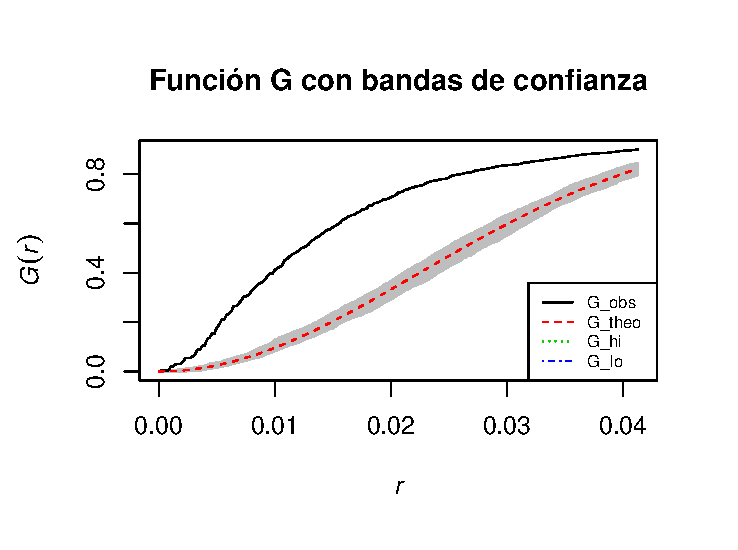
\includegraphics[scale=0.7]{../Imagenes/FuncionG}
    	\caption{Intervalos de confianza\\  y valores observados de la función G}
    	\label{G1}
    \end{figure} 


   En la figura \ref{G1} se presenta el gráfico de la función $G$, en él se ve claramente  que la función  observada se encuentra muy distanciada de la función $\hat{G}$ estimada bajo AEC.  Estadísticamente se establece que al nivel de significancia del 2$\%$ el patrón de puntos no es  Proceso Homogéneo de Poisson; además, la función $G$ crece rápidamente indicando patrón de agregación. \\      
	 
			
			
				\textbf{Cálculo de la Función $F$}\\
			
	Esta función implementa la mínima distancia de un punto arbitrario del espacio al  evento más cercano (mínima distancia punto-evento). Conocida también como función del espacio vacío. 	El cálculo de la función $F$ se llevó a cabo mediante el comando  {\ttfamily envelope(Oriente, Fest)},  que genera una simulación de Monte Carlo de un proceso con distribución  Aleatorizada Espacial Completa (AEC)  o   Proceso Homogéneo de Poisson (PHP), con intervalos de confianza del $ 98\% $.
	 			
			\begin{figure}[h!]
				\centering
				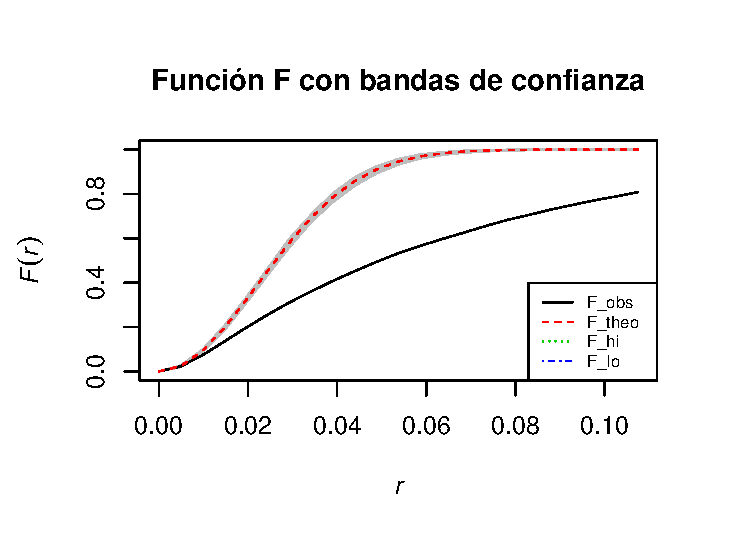
\includegraphics[scale=0.7]{../Imagenes/FuncionF}
				\caption{Intervalos de confianza \\ y valores observados de la función F}
				\label{F1}					
			\end{figure}
			
   En la figura \ref{F1} se presenta el gráfico de la función, en él se ve claramente la función $F$ observada se encuentra por debajo de la función $\hat{F}$ estimada bajo AEC, con crecimiento lento respecto del valor esperado de $\hat{F}$  bajo AEC.  En este caso se establece estadísticamente al nivel de significancia del 2$\%$ el patrón de puntos no se ajusta a un Proceso Homogéneo de Poisson; además, el crecimiento lento y por debajo indicando posible patrón de agregación.\\   
  
  					
			
				\textbf{Cálculo de la Función $K$ y  $L$}\\
			
	Esta función conocida también como la función de Ripley, mide el número de eventos que se encuentran dentro de una distancia dada a cualquier evento particular. El cálculo de la función $K$ se llevó a cabo mediante el comando  {\ttfamily  envelope(Oriente, Kest, r = r, nrank = 2, nsim = 99)},  que genera una simulación de Monte Carlo de un proceso con distribución  Aleatorizada Espacial Completa (AEC)  o   Proceso Homogéneo de Poisson (PHP), con intervalos de confianza del $ 96\% $. 
		
		Para analizar este estadístico se gráfica la función $K$ con los datos observados  vs la función $\hat{K}$ estimada bajo AEC, mediante la simulación y sus intervalos de confianza.  
		
		
		\begin{figure}[h!]
			\centering
			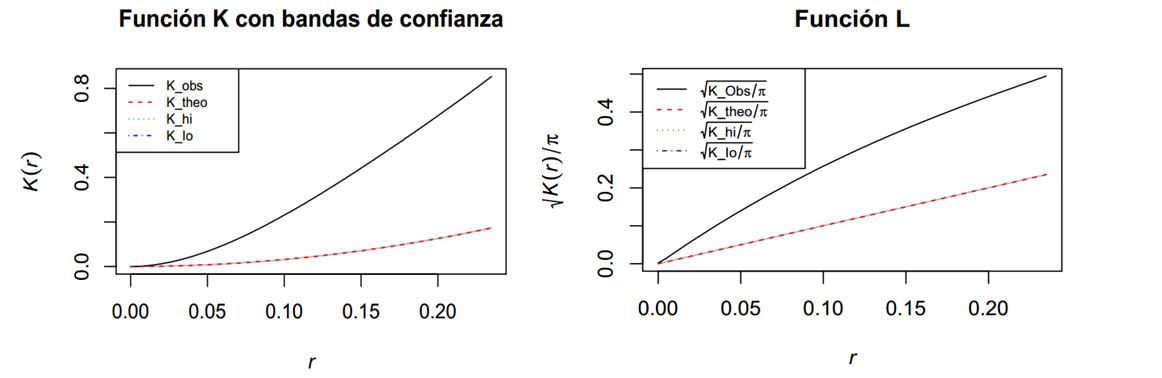
\includegraphics[scale=0.65]{../Imagenes/KyL}
			\caption{Intervalos y valores observados de la función $K$ y $L$}
			\label{KyL}					
		\end{figure}
		
		
		En la figura \ref{KyL} se presenta el gráfico de la función, en él se observa que la función $K$ se encuentra muy distanciado de la función $\hat{K}$ estimada bajo AEC y sus intervalos de confianza.  En este caso se establece estadísticamente al nivel de significancia del $4\%$ el patrón de puntos no se ajusta a un Proceso Homogéneo de Poisson; además, como la función $K$ está por encima de $\hat{K}$ indica patrón de agregación.\\   
		
							
		
		La función $L$ es una manipulación de la función $K$ de Ripley, consiste en restar la función $K$ observada  menos el valor teórico bajo AEC; el resultado debe ser la función constante cero, si el proceso puntual es homogéneo.
		El cálculo de la función $L$ se llevó a cabo mediante la aplicación de la fórmula $\cdot - pi * r^{2}$ en el comando para  gráficar 
		 {\ttfamily{  plot(K, . - pi*r\^{}\{2\} \~{} r, legend=F,  main="Función L")  }},  
		  que genera el gráfico con la simulación de Monte Carlo y los intervalos de confianza del $ 96\% $, y la función $L.$  		 
	 
	

		
			\begin{figure}[h!]
			\centering
			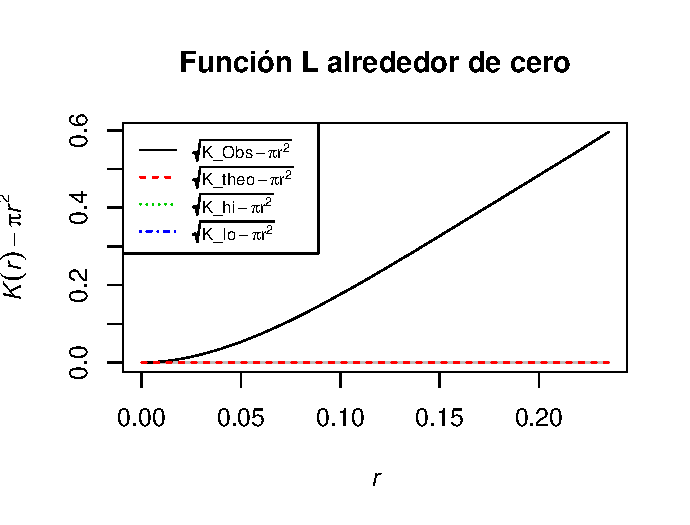
\includegraphics[scale=0.7]{../Imagenes/FuncionL2}
			\caption{Intervalos de confianza  \\ y valores observados de la función $L$}
			\label{L2}					
		\end{figure}
		
		
		
		
		
		
		En la figura \ref{L2} se muestra el gráfico de la función $L$, donde se observa que la función se encuentra distanciada de la función $\hat{L}= 0$ estimada bajo AEC y sus intervalos de confianza.  En este caso se establece estadísticamente al nivel de significancia del $4\%$ el patrón de puntos no se ajusta a un Proceso Homogéneo de Poisson; además, como la función $L$ está por encima de $\hat{L}$ indica patrón de agregación.\\   
		
		
			%%  el colombiano tomo las notas de Babdely pagina 95 
			%%  A Pearson residual of −14 is a gross departure from the fitted model.
			%%  Muy bueno el text de   Baddley, espaecial para modelos y ajustes 
			
			
			
			\subsection{Conclusión obtenida con los indicadores de aleatorización espacial completa}
		
  De acuerdo con los resultados obtenido con el método de los cuadrantes, y los  Índices basados en la distancia $G, F, K, $ y $ L,$  se concluye que el proceso puntual en estudio no sigue el comportamiento de un Proceso puntual homogéneo. Este resultado no es tan inesperado, ya que generalmente los fenómenos naturales tratados como los procesos espaciales reales no se comportan como un Proceso puntual homogéneo.\\
	
  Finalmente, se puede concluir que los eventos sismológicos ocurridos zona Nor-oriental de Venezuela, durante el periodo  09/01/1995 al  02/10/2018, no cumplen la hipótesis de aleatoriedad espacial completa,  y se comportan como un proceso agregado y no como un proceso homogéneo de Poisson.\\

  El próximo paso en esta investigación es calcular la intensidad del proceso, que de acuerdo con los resultados de los estadísticos el fenómeno no es homogéneo en el área de estudio (ventana de observación). La siguiente sección \ref{Intensidad_kernel}  se dedica al análisis de la intensidad del proceso.\\
		

		
	\section{Análisis de la intensidad espacial del proceso}\label{Intensidad_kernel}
	
	En la sección \ref{distancia},  se llevó acabo el análisis de los índices de aleatoriedad espacial, calculado bajo la hipótesis de nula de AEC; en este caso la intensidad es considerada constante, el resultado de la estimación bajo ésta hipótesis  fue $\lambda = 321.8537$;  para el caso del método de los cuadrantes bajo la misma hipótesis, la intensidad  que resultó fue igual  a   $366.6,$ de acuerdo con el número de cuadrantes seleccionados.  Sin embargo, debido a los resultados estadísticos esta hipótesis de intensidad constante no es útil en el proceso analizado, debido a que el proceso no es homogéneo, en consecuencia la intensidad  varía en el área de interés. Para estimar la intensidad del proceso (no homogéneo) se emplea el método del Kernel, que se desarrolla continuación. \\ 
	% determinar la cantidad de variación espacial de la intensidad.
	
	
	\textbf{Cálculo de la intensidad por el método del kernel}\\
	
	Para el cálculo de la intensidad  el paquete spatstat tiene el comando {\ttfamily  $density(\cdot$)}, que se aplica al objeto {\ttfamily  ppp}. En este caso se usó con un ancho de ventana $h$ igual a $0.20$, obtenido éste por el método empírico de ensayo y error (Aunque hay un comando para ayudar a encontrar el valor de $h$).El resultado se presenta en tres gráficos, gráfico del kernel, el de contornos o  curvas de nivel y en tres dimensiones generado con el comando  {\ttfamily  persp( $\cdot$)}.
	
	
	
	\begin{figure}[h!]
		\centering
		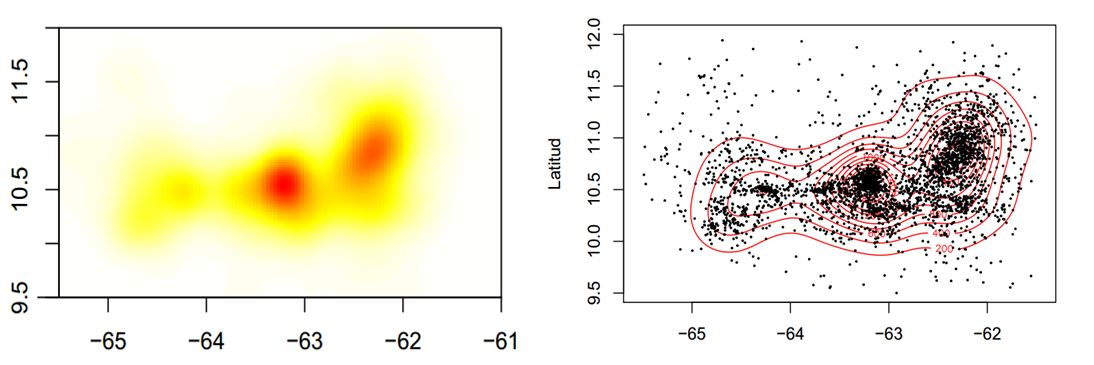
\includegraphics[scale=0.6]{../Imagenes/Int1y2N}
		\caption{ Densidad de sismos y mapa de contorno   }
		\label{Int1y2}
	\end{figure}
	

	
	
	
	En la figura \ref{Int1y2}  se muestra el gráfico de la intensidad con la técnica del suavizado de  kernel  y  en contornos, ambos calculado con un ancho de banda igual a 0.20, y se agregan los puntos del proceso al grafico de contornos; mientras que la figura  \ref{Int3}   presenta la estimación de la  intensidad (técnica de suavizado de  kernel) en tres dimensiones, generando este último una impresión de la variación espacial local visual muy clara.\\
	\begin{figure}[h!]
		\centering
		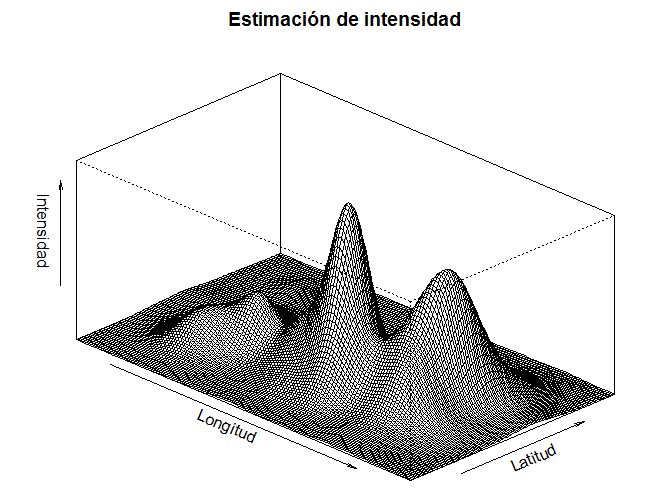
\includegraphics[scale=0.6]{../Imagenes/K015}              %   K020JEPG
		\caption{Estimación de intensidad en tres dimensiones}
		\label{Int3}
	\end{figure}
	%     \includegraphics[scale=0.7]{../Imagenes/K015jpeg}  con ancho de banda 0.15

				
 Como se observa en estas tres gráficas la intensidad no puede ser es homogénea, presenta variabilidad en el área de estudio. Con fuerte incidencia en la zona central del Edo Sucre, específicamente en zona donde se encuentra la población de Carúpano.
		
%  Estas tres graficas aportan más información sobre  comportamiento de la intensidad del proceso, indicando que la intensidad puede no ser no es homogénea , como lo resulto en los índices de AEC.			
		
 En la  sección \ref{APIs} se visualiza la intensidad espacial sobre el mapa de la zona de interés, con las técnicas densidad del kernel que ofrece el  software R y API's o servidores Web de mapas libres.  
		

  \subsection{Análisis descriptivo de la intensidad en la región}\label{APIs}

   Luego de  confirmar en la sección \ref{Intensidad_kernel}, que la intensidad del proceso no es homogénea; esta sección  se dedica al estudio descriptivo de la intensidad del proceso mediante la técnica del kernel, empleando una interfaz de programación de aplicaciones (API's) para obtener los mapas, necesario para visualizar  la intensidad. En principio se planifico el trabajo con googleMap, pero debido a la situación país no fue posible usar esta API’s, en su lugar se empleó la API’s  de Stamen, un proveedor de mapas libres que usa datos de OpenStreetMap. Los resultados en mi consideración son  muy buenos, se logra exponer el comportamiento del fenómeno en forma visual con gran claridad, en este caso se ilustra la representación de la intensidad sobre el mapa en la  zona de estudio, permitiendo comprender el fenómeno en forma muy didáctico.\\


   Para el cálculo de la intensidad, se empleó  el paquete spatstat para limpiar y organizar la data, los paquetes ggmap, qmplot para obtener mapas y ggplot3 para manipular la estética del mapa con la intensidad mediante la técnica del suavizado de kernel, con curvas de contorno y en tres dimensiones. En la próxima parte presenta los mapas obtenidos y se analiza la intensidad.\\
   %  código de r {   { \ttfamily   get$\_$stamenmap(\cdot)}}   


 \textbf{Análisis descriptivo de la intensidad, visualizada en el mapa de la región}\\

    En las figuras \ref{julio2019_14} y \ref{CurvasRojasqplot} se muestra el resultado de la aplicación de la técnica del kernel, presentación en suavizado de kernel y curvas de contorno respectivamente.\\
    \begin{figure}[h!]
	\centering
	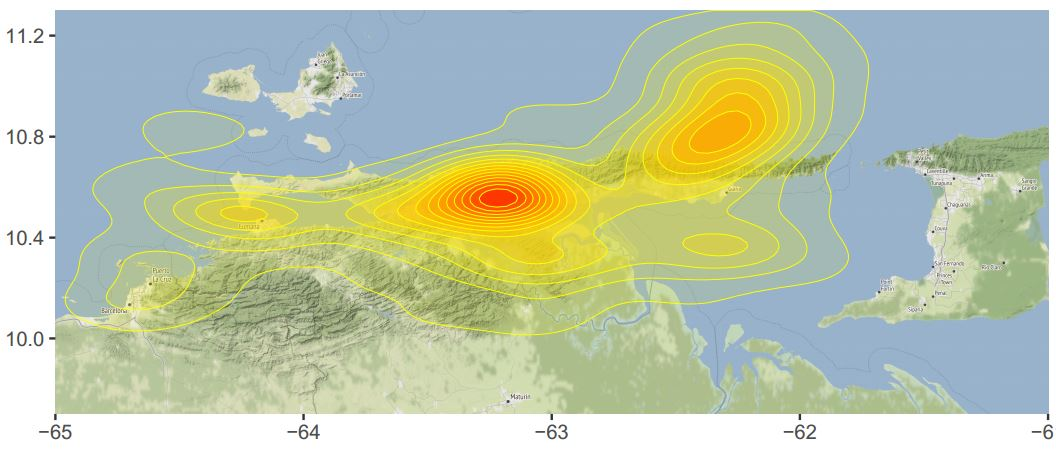
\includegraphics[width=1\linewidth, height=0.34\textheight]{../Imagenes/MapaDefinitivo06}
	\caption[Estimación de la intensidad por la técnica del Kernel, visualizado sobre el mapa]{Estimación de la intensidad  mediante la técnica del Kernel.} \vspace{-0.5cm}
	\caption*{  {\scriptsize  {\ttfamily  Mapa obtenido de la API's de Stamen}} }
	\label{julio2019_14}
   \end{figure} En estos dos gráficos  se observa claramente que la mayor intensidad del proceso sísmico tratado en   esta investigación se encuentra en la zona central del estado Sucre,específicamente en la zona donde se encuentran los municipios Bermúdez (Carúpano),  Andrés Eloy Blanco (Casanay),  Andrés Mata (San José de Aerocuar), Benítez (El Pilar) y Libertador (Tunapuy). 
    \begin{figure}
	\centering
	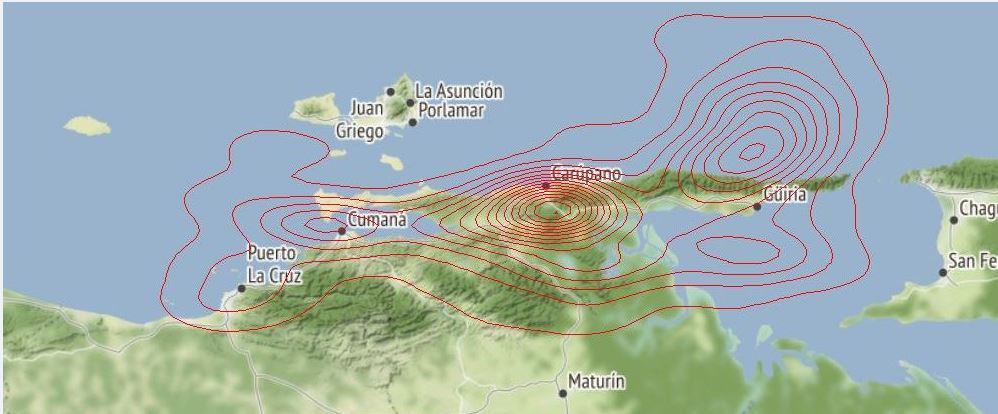
\includegraphics[width=1\linewidth, height=0.34\textheight]{../Imagenes/Manipulado2}
	\caption[Curvas de contorno, con la técnica del Kernel]{Curvas de contorno, con la técnica del Kernel }
	\label{CurvasRojasqplot}
    \end{figure}    La segunda zona en intensidad se observa en el mar caribe, al norte de la población de Güiria,  municipio Valdez; y la tercera zona en intensidad se encuentra prácticamente sobre Cumaná y la península de Araya, hacia el sector denominado Punta Araya.   La cuarta zona en intensidad se observa en el golfo de Paria, al Sur las poblaciones de  Irapa y  Güiria, municipios Valdez y  Mariño respectivamente. Otras zonas con menor intensidad se observa en el estado Anzoátegui, específicamente en la ciudad Puerto La Cruz y Barcelona; y al Sur-Oeste de la isla de Margarita.\\


\begin{figure}[h!]
	\centering
	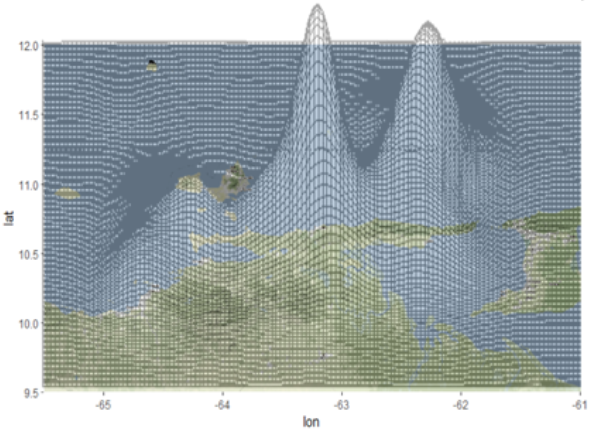
\includegraphics[width=1\linewidth, height=0.34\textheight]{../Imagenes/Mapa_Intensidad01}
	\caption[Estimación de la intensidad por la técnica del Kernel, visualizado sobre el mapa en 3D]{Estimación de la intensidad  mediante la técnica del Kernel.} \vspace{-0.5cm}
	\caption*{  {\scriptsize  {\ttfamily Visualizado sobre el mapa en 3D}} }
	\label{Septiembre2019_14}
\end{figure}


   En forma general los eventos sísmicos se observan a lo largo del estado Sucre de Este a Oeste, aproximadamente en una banda entre 10.3 y 10.8 de latitud; observándose cierta concentración al este del estado entre la Ciudad de Cumaná y salida del golfo de Cariaco,   y una  gran incidencia en la zona central del estado, donde se encuentra la población de Carúpano; y una segunda muy notable al norte de la población de Güiria (municipios Valdez) (ver figura \ref{Septiembre2019_14}), hacia el mar Caribe (zona limite de las placas tectónica). Es muy importante señalar que estos eventos se observan ubicados prácticamente sobre la Falla Sísmica  de El Pilar (Ver figura \ref{Pilar}); además esta región se encuentra en una zona  límites de las Placa del Caribe y la Placa Suramérica (Ver figura \ref{Esquema}). En la Figura \ref{Placas}, se muestra un mapa en el que se representan esquema de límites de placas para Venezuela.\\





\textbf{Sistema de fallas sismogénicas en Venezuela}\\

Según La Fundación Venezolana de Investigaciones Sismológicas (FUNVISIS), como órgano oficial encargado de realizar y promover en forma permanente investigaciones y estudios sismológicos, expone que en Venezuela, la zona de mayor actividad sísmica corresponde a una franja de  aproximadamente 100 Km. de ancho, definida por los sistemas montañosos de Los  Andes, la Cordillera Central y la Cordillera Oriental; a través de los cuales se identifica el principal sistema de fallas sismogénicas del país, formado por las fallas  de Boconó (Los Andes), San Sebastián (Cordillera Central) y El Pilar (Cordillera  Oriental), que constituyen el límite principal entre la placa del Caribe (al norte) y la  placa de América del Sur (al sur) (ver figura \ref{Placas}),   razón por la cual ha sido este sistema de fallas el origen de los sismos más severos que han afectado al país, pudiendo llegar a generar  un sismo máximo probable de magnitud 7.8 con períodos de retorno de 300 a 400 años. (Alfonso Malaver, 1995)\\

La Falla de Boconó, se extiende desde el sur del Estado Táchira con dirección
noreste, hasta la costa con el Mar Caribe, atravesando longitudinalmente la Cordillera
de Los Andes Venezolanos a lo largo de una distancia que supera los 500 Km. Según Funvisis, el Sistema de Fallas de Boconó esta vinculado con los sistemas de Fallas de San Sebastián y de El Pilar, lo que define una franja de alta sismicidad de más de 1000 Km. de longitud y de aproximadamente 100 Km. de ancho, en la que habita cerca del 80\% de la población de Venezuela y que afecta algunas de las ciudades más importantes del país, tales como San Cristóbal, Mérida, Barquisimeto, Caracas y Cumaná, entre otras.

Los sistemas de fallas de Boconó - San Sebastián - El Pilar, han sido propuestos como el límite principal entre las Placas Caribe y América del Sur (ver figura \ref{Esquema}), causante de los sismos más severos que han ocurrido en el territorio nacional; además de este sistema de fallas, existen otros accidentes activos menores, como: Oca-Ancón, Valera, La Victoria y Urica, capaces de producir sismos importantes. En la Figura   \ref{Esquema}, se muestra un mapa en el que se representan las principales fallas activas en Venezuela, en un esquema  del movimiento de las placas tectónicas para Venezuela.

		
		
		
			\section{Modelo propuesto}
		
  Las pruebas estadísticas de aleatoriedad espacial completa desarrolladas en la sección \ref{Puntuales},   indican que el proceso no presenta el comportamiento de un  proceso  homogéneo de Poisson;  además,  estas pruebas indican que el comportamiento del proceso es de forma agregada, por lo que la estructura de los datos debe ajustarse a un modelo que cumpla con esta característica.  
  
  Los modelos que  aparentan tener esta característica son:  los modelos de  Poisson no homogéneo,  el modelo de Poisson con clúster y el proceso de Cox.  Mientras que los modelos como el Homogéneo, el de inhibición simple y el de  Markov, corresponden a proceso aleatorios, con cierta regularidad o uniformes entre sus ubicaciones, por tal razón no serán objeto de análisis. 

  En el caso del proceso de Cox, la función de intensidad es aleatoria, es decir,  está dirigida por de un proceso estocástico en la región; sin embargo,  la intensidad espacial sísmica observada se comporta de acuerdo a un proceso clústers en áreas bién definidad{\footnote{Presentan clústeres, siguiendo el proceso tectónico o la Falla de El Pilar}}, siguiendo el patrón de falla de El Pilar.  Por lo tanto, se descarta el modelo de Cox.  

  El proceso agregado de Poisson es un modelo que incorpora explícitamente la formación de clúster. Claramente el proceso en estudio,  las ubicaciones de los sismos  también presentan clústeres. Sin embargo, el modelo agregado de Poisson supone que la ubicación de los eventos principales, o padres, se comportan de manera aleatoria. En cambio, las agrupaciones sísmicas entre sí siguen un comportamiento particular de acuerdo a la falla tectónica de El Pilar o placas{\footnote{Placa del Caribe y la Suramérica, y Falla de El Pilar }}. En este sentido, no se puede  considerar este proceso como un  modelo como agregado de Poisson.


  El proceso no homogéneo de Poisson supone que la intensidad varía en función de la localización geográfica, y factores propios del fenómeno, es decir, el proceso no es estacionario.  Los movimientos sísmicos tienden a agruparse en la zona central del estado Sucre, a los largo del Este al Oeste, con tendencia al Noroeste (norte de la población de Güiria, municipios Valdez)  hacia sobre el mar caribe. Observándose  pocos eventos (probabilidad baja de que ocurra un evento sísmico) en las regiones del sur, hacia el Amazona. En este caso, la función de intensidad debe estar  relacionar  con  una covariable asociada a la ubicación de los eventos, que para el objeto del proyecto corresponde a las fallas geológicas{\footnote{Falla de El Pilar, y placas tectónicas}} de  la zona.
  
   
   Se puede observar la intensidad del proceso cerca o sobre de la falla de EL Pilar (\ref{Pilar}), formando conglomeraciones en torno a ella (ver figura \ref{Septiembre2019_14}).    De acuerdo a las características es válido suponer que el proceso no homogéneo de Poisson es un modelo para la ocurrencia y magnitud de sismos en la zona Oriental de Venezuela. 


			\section{Conclusiones}{\label{Conclucion} }
			

  La aplicación de las técnicas de estadística espacial y el uso del software {\ttfamily R} como un sistema de información geográfica (SIG), permitió con gran facilidad la exploración,  análisis y visualización  en el mapa de la data georeferenciada, y obtención de  resultados estadísticamente significativos,  del proceso de eventos sísmicos ocurridos zona Oriental de Venezuela, durante el periodo  09/01/1995 al  02/10/2018.	

  Los resultados del análisis descriptivo del proceso  manifiestan una situación poco favorable a lo que se supone es un proceso Homogéneo de Poisson, esta situación se confirma con los índices de aleatoriedad espacia. Con el método de los cuadrantes, el estadístico chi-cuadrado generó un  $P$ valor muy bajo  {\ttfamily ($p-value < 2.2e-16 $)}, rechazando la hipótesis de aleatoriedad espacial. En el caso de los índices basados en las distancias el resultado fue el mismo; el resultado de los índices $G$ y $F$  establece estadísticamente al nivel de significancia del 2$\%$  que el patrón de puntos no se ajusta a un Proceso Homogéneo de Poisson; además, el índice en ambos casos indica  patrón de agregación. En el caso del índice $K$ (y sus formas alternativas  $L$ y $L$ al rededor de cero) se establece  estadísticamente al nivel de significancia del $4\%$ que el patrón de puntos no se ajusta a un Proceso Homogéneo de Poisson, indicando también  patrón de agregación.
  
  De esta forma se concluye:\\	
	\begin{itemize}	
\item   El proceso de eventos sísmicos ocurridos zona Orienta de Venezuela, durante el periodo  09/01/1995 al  02/10/2018, no cumplen la hipótesis de aleatoriedad espacial completa,  y se comportan como un proceso agregado y no como un proceso homogéneo de Poisson.

\item  Como consecuencia  de este resultado, la intensidad del proceso no es  homogénea, situación que se confirma con el estudio descriptivo de la intensidad del proceso mediante la técnica basado en el Kernel.\\    
\end{itemize} 

  \textbf{Conclusión sobre los eventos sísmicos en la región y zonas con mayor intensidad sísmica}\\

 
 
\begin{itemize}
 
\item   Con los resultados obtenidos con la técnica del Kernel, se concluye que la mayor intensidad del proceso sísmico tratado en esta investigación se encuentra en la zona central del estado Sucre, específicamente en la zona donde se encuentran los municipios Bermúdez (Carúpano),  Andrés Eloy Blanco (Casanay),  Andrés Mata (San José de Aerocuar), Benítez (El Pilar) y Libertador (Tunapuy). La segunda zona en intensidad se observa en el mar caribe, al Norte de la población de Güiria,  municipio Valdez; y la tercera zona en intensidad se encuentra prácticamente entre Cumaná y el sector denominado Punta Araya de península del mismo nombre.  La cuarta zona en intensidad se observa en el golfo de Paria, al Sur las poblaciones de  Irapa y  Güiria, municipios Valdez y  Mariño respectivamente. Otras zonas con menor intensidad se observa en el estado Anzoátegui, específicamente en la ciudad Puerto La Cruz y Barcelona; y al Sur-Oeste de la isla de Margarita.\\

  
 
\item   En forma general los eventos sísmicos se observan a lo largo del estado Sucre de Este a Oeste, aproximadamente en una banda entre 10.3 y 10.8 de latitud; observándose cierta concentración al Este del estado Sucre, ubicado específicamente entre la Ciudad de Cumaná y el sector denominado Punta Araya en la península del mismo nombre;  la mayor  incidencia se observa en la zona central del estado, donde se encuentra la población de Carúpano; y una segunda muy notable al norte de la población de Güiria (municipios Valdez), hacia el mar Caribe (zona limite de las placas tectónica). Es importante señalar que estos eventos se observan prácticamente  sobre la falla sísmica  de El Pilar; además, de encontrarse en la zona de límites de Placa del Caribe y la Placa Suramérica. \\
 
 
 
 \item  Se propone como modelo para la ocurrencia de sismos en la zona Oriental de Venezuela el Proceso no Homogéneo de Poisson. 
  El proceso no homogéneo de Poisson supone que la intensidad varía en función de la localización geográfica, y factores propios del fenómeno. 
  
\end{itemize}

	\section{Recomendaciones }{\label{Recomendacion} }



   Luego de analizar el proceso de eventos sísmicos de la zona oriental de Venezuela, y observar la incidencia de eventos en la zona, es necesario recomendar a las autoridades  y entes públicos que tienen la responsabilidad de velar por la seguridad ciudadana en caso de emergencia causadas por desastre naturales, tomar mayor conciencia y precaución con respecto al problema del riesgos sísmico que estamos sometidos. 
 
   En tal sentido es importante señalar la necesidad de mantener una cultura informativa permanente referente a prevenir accidentes en caso de un sismo de gran magnitud.
   % o tsunamis en el caso de zonas costeras, como penuisula de paria. 
 
  Mayor vigilancia  con respecto al  cumplimiento de las normas para desarrollar construcciones residenciales, recintos escolares, centros comerciales y lugares públicos. Evitando la vulnerabilidad sísmica{\footnote{\scriptsize  Norma de construcción antisísmica vigente (NSR-10, establecida mediante Decreto 926 de 2010 y sus respectivas modificaciones, ej. Decreto 945 de 2017)}}, que  está relacionada con la capacidad de una edificación (o la población) para resistir el daño frente a la amenaza sísmica. \\

 %	{\tiny   diminuto 
 	
 %	{ \scriptsize  { \ttfamily  

 
  Con este trabajo se muestra el uso de la tecnológica del software libre en el estudio espacial  de fenómenos naturales, tanto en de estadística espacial como la implementación de los sistemas de información geográficos (SiG); en este caso se emplea el software R (version 3.5.1) al campo de la Sismología; sin embargo, hay una inmensa variedad en software libre para aplicar de las técnicas de estadística  espacial y SIG, en las diferentes áreas de conocimiento,  como el software Python, GVsig, Qgis, CrimeStat, etc.  Además,  permiten la manipulación de gran volumen de información, técnica conocida como data mining  o minería de datos (Big Data). En tal sentido, se recomienda la implementación de la estadística espacial, conjuntamente con un sistema de información geográfica (GIS) y el software libre, en el estudio de procesos espaciales o  fenómenos naturales. \\



\newpage

 
			\chapter*{Anexo }	
	            	\addcontentsline{toc}{chapter}{Anexo }
		
		\begin{figure}[h!] 
			\centering   	
			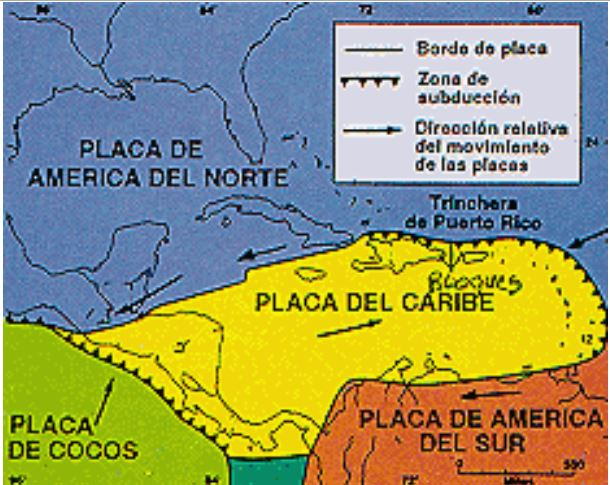
\includegraphics[scale=0.95]{../Imagenes/Placas}
			\caption[Placas Tectónicas que afectan América y el Caribe]{Placas Tectónicas que afectan América y el Caribe}\vspace{-0.4cm}
			\caption*{{ \scriptsize  {\ttfamily (http://www.infocentros.org.sv/terremotos/) }}}
			\label{Placas}
		\end{figure}
		
		Placas Tectónicas que afectan parte de América y el Caribe, y su movimiento.
		
	\newpage
		
			
		
		\begin{figure}[h!]    	
			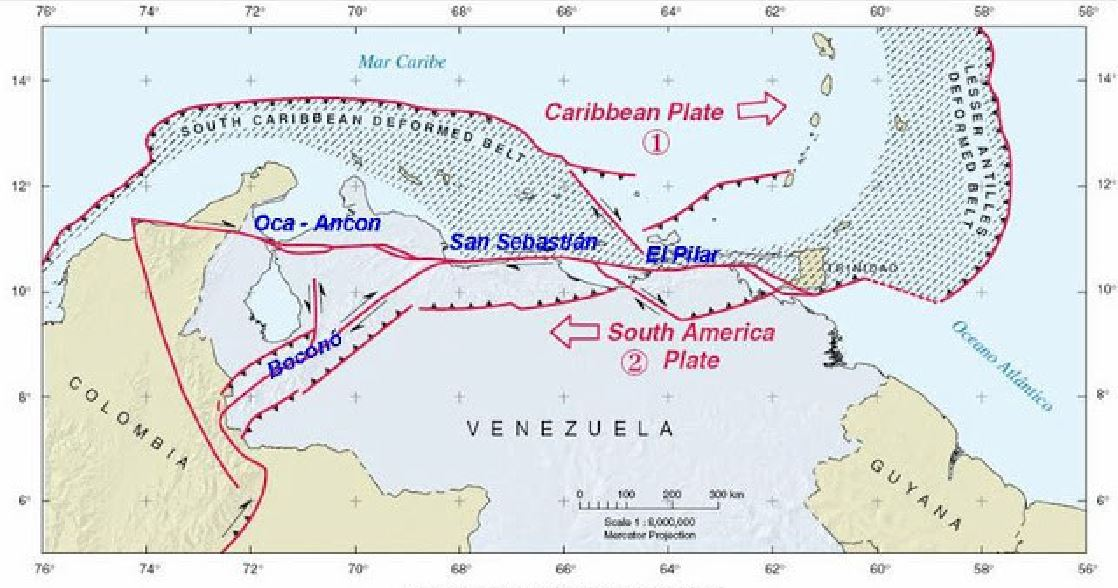
\includegraphics[scale=0.65]{../Imagenes/Falla_C}
			\caption[Falla cuartenaria]{Esquema de límites de placas para Venezuela}\vspace{-0.4cm}
			\caption*{{ \scriptsize  {\ttfamily  (http://www.funvisis.gob.ve/old/images/mapas/fallas$\_$cuaternarias.png)}} 	}
			\label{Esquema}
		\end{figure}
		Movimiento relativo de Placa del Caribe respecto a la Placa Suramérica en 1 es de 12,7 mm/a en dirección 88,48\\ 
		
		Movimiento relativo de Placa Suramérica con respecto a la Placa del Caribe en 2 es de 14,2 mm/a en dirección 270,48  
		
				
			
			
			\begin{landscape}
				\thispagestyle{empty}
				\begin{figure}[h!]    	
					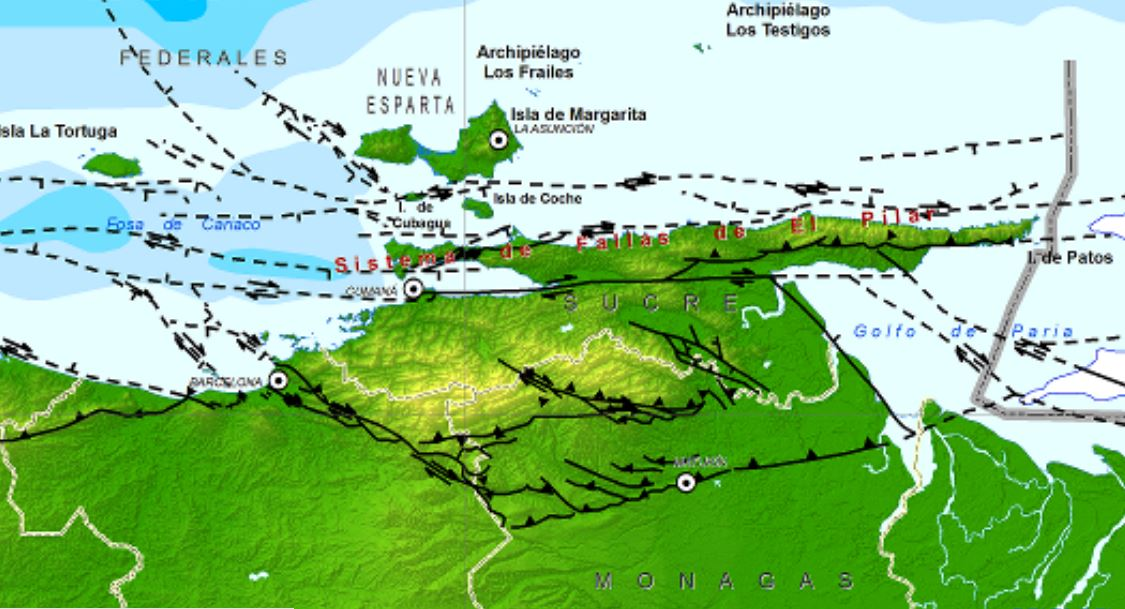
\includegraphics[width=1.125\linewidth, height=0.95\textheight]{../Imagenes/Pilar}
					\caption[Falla de El Pilar]{ Falla de El Pilar.    {\scriptsize  {\ttfamily  (http://www.funvisis.gob.ve/old/images/mapas/fallas$\_$cuaternarias.png)}} 	}
					\label{Pilar}
				\end{figure}
			\end{landscape}

				






\newpage


				\chapter*{Términos Glosario}
					\addcontentsline{toc}{chapter}{Términos Glosario }
			%	Tile baldosa teja.   Tie: empatar hacer, nudo\\
				{\bf{API's}}\\
			Una interfaz de programación de aplicaciones (API) es un término amplio que define 
			las reglas que guían su interacción con algún software.   \\
				
			
				%Una interfaz de programación de aplicaciones (API) es un término amplio que define 	las reglas que guían su interacción con algún software.		Google Cloud Platform, la plataforma de Google en la nube.....   			Google Earth™, Google Maps™ and Other Formats  texto roger pag 108	
			
				
				{\bf{Software privado}}\\ 
				
				
				{\bf{SQL Server}}\\
				SQL server es el servidor de bases de datos de Microsoft. Dispone de soporte para datos espaciales y un tipo de dato geometry para almacenamiento de datos espaciales.\\
				
				{\bf{DB2 Spatial Extender}}\\
				DB2 Spatial Extender es una extensión para la base de datos DB2 de IBM que implementa los tipos de datos y funciones definidas por ISO SQL/MM y el OGC. Está disponible tanto para Windows como para Linux, y las principales aplicaciones SIG ofrecen acceso a esta base de datos.\\
				
				{\bf{ArcCatalog}}\\
				ArcCatalog es la herramienta de ESRI para la creación y mantenimiento de metadatos. Permite la creación de metadatos según los estándares ISO y FGDC, aunque pueden extenderse sus funcionalidades para adaptarse a otros esquemas distintos. Por ejemplo, existe un modulo que permite la creación de datos conforme al núcleo español de metadatos. El programa incluye funcionalidades de importación y exportación, así como otras que lo conectan a distintos elementos de la familia de productos ESRI.\\
				
				\index{ArcMAP}
				{\bf{ArcMAP}}\\
				ArcMAP es el principal componente del conjunto de aplicaciones ArcGIS de ESRI, y el que contiene las funcionalidades clásicas del SIG de escritorio, respondiendo a la definición de este. ArcMAP es una herramienta que permite la visualización y manejo de información geográfica, y que cuenta con una arquitectura extensible mediante la que pueden añadírsele nuevas funcionalidades. Existen numerosos paquetes adicionales proporcionados por ESRI, con los cuales las capacidades de ArcMAP pueden extenderse hasta cubrir la práctica totalidad de capacidades que un SIG plenamente productivo en cualquier ámbito debe presentar hoy en día. Algunos de los paquetes más destacados son los correspondientes a las funciones de análisis, tales como Spatial Analyst (análisis ráster), 3D Analyst (análisis 3D y de relieve) o Geostatistical Analyst (geoestadística).\\
				
				{\bf{GeoMedia}}\\
				Geomedia es el SIG de escritorio de la empresa Intergraph, y producto principal de su familia de aplicaciones. Se trata de un SIG completo con capacidades de manejo de datos, visualización, análisis y funciones avanzadas de creación de cartografía. Permite el acceso a datos remotos mediante estándares OGC y puede extenderse empleando herramientas de programación sencillas. Geomedia está particularmente enfocado para un uso industrial, respondiendo a las necesidades de grandes organismos y empresas tales como compañía de telecomunicaciones o de suministros, que trabajan con grandes cantidades de datos.\\
				
				{\bf{ArcGISServer}}\\
				ArcGISServer es la tecnología de la empresa ESRI para distribuir servicios Web basados en información geográfica. Soporta el uso de estándares OGC y W3C, aunque también cuenta con sus propios formatos para cada uno de los servicios que es capaz de proveer. Estos van desde los habituales servicios de mapas hasta servicios de edición cartográfica (usando el estándar WFS–T) o servicios de geoprocesamiento avanzado, cubriendo en conjunto la práctica totalidad de servicios que actualmente se utilizan y convirtiendo a este servidor en uno de los más completos del mercado.\\
				
				{\bf{ArcIMS}}\\
				ArcIMS es el nombre de la tecnología de ESRI para los servicios de mapas. Dado que ArcGISServer es un producto más completo y puede ofrecer otros servicios además del de mapas, ArcIMS es ya un producto obsoleto, aunque muy presente en el mercado. ESRI, no obstante, no provee ya servicio para este servidor, recomendando la adopción de ArcGISServer.\\
				
				
				{\bf{Mapinfo}}\\
				Mapinfo  es un SIG de escritorio completo, con especial atención a las funcionalidades de creación y edición de datos, y producción de cartografía. Es capaz de conectarse a bases de datos espaciales y posee módulos de uso sencillo que permiten la publicación de cartografía en Internet, tanto mediante mapas estáticos como mediante mapas interactivos.\\
				
				{\bf{Google Earth}}\\
				Google Earth no es un SIG de escritorio propiamente dicho, ya que carece de gran parte de las funcionalidades que caracterizan a estos. Se trata básicamente de un globo 3D que permite visualizar cartografía propia, acceder a servicios WMS y, especialmente, explorar la cartografía ofrecida por Google, en la cual se incluyen imágenes de alta resolución de todo el globo, así como otras capas con información variada, tales como calles o puntos de interés, entre otras.\\
				
				{\bf{Google Mapas}}\\
				Más que un cliente Web para visualización de mapas, Google Mapas es un servicio de cartografía Web que dispone de una interfaz de programación mediante la cual puede emplearse para la creación de servicios relacionados. Google Mapas incluye datos (imágenes aéreas con cobertura global a excepción de las zonas polares) y un cliente Web para visualizar esas imágenes, el cual permite a su vez, y a través de esa interfaz de programación, ciertas funcionalidades adicionales tales como la creación de puntos de interés o el cálculo de rutas óptimas.\\
				
				
				{\bf{OpenStreetMap  }}{\footnote{Tomado de  Wikipedia}} \\
			OpenStreetMap (también conocido como OSM) es un proyecto colaborativo para crear mapas editables y libres. En lugar del mapa en sí, los datos generados por el proyecto se consideran su salida principal.
			
			Los mapas se crean utilizando información geográfica capturada con dispositivos GPS móviles, ortofotografías y otras fuentes libres. Esta cartografía, tanto las imágenes creadas como los datos vectoriales almacenados en su base de datos, se distribuye bajo licencia abierta Licencia Abierta de Bases de Datos (en inglés ODbL).\\			
		
		En octubre de 2014 en el proyecto estaban registrados en torno a 1.840.000 usuarios, de los cuales alrededor de 22.600 realizaban alguna edición en el último mes.  Los usuarios registrados pueden subir sus trazas desde el GPS y crear y  	corregir datos vectoriales mediante herramientas de edición creadas por la comunidad OpenStreetMap.  Cada semana se añaden 90.000 km de nuevas carreteras con un total de casi 24.000.000 km de viales (febrero de 2011), eso sin contar otros tipos de datos (pistas, caminos, puntos de interés, etc.). El tamaño de la base de datos (llamada planet.osm) se situaba en julio de 2017 por encima de los 800 gigabytes.\\
		
			
				                                                                  %  (58 GB con compresión bzip2).\\	
				{\bf{StamenMap}}\\
        	Stamen (stamen.com) es un estudio de diseño y desarrollo ubicado en San Francisco, Estados Unidos, enfocado a la generación y visualización de mapas a partir de datos cartográficos. Stamen\footnote{https://wiki.openstreetmap.org/wiki/ES:Stamen}  emplea en gran medida los datos de OpenStreetMap en muchas de sus visualizaciones de mapas y ha proporcionado tres juegos de teselas: Tóner, Terreno y Acuarela.\\
				
				
				
				
				
				{\bf{ Software libre}}\\
				
				
				{\bf{ PostGIS}}\\
				PostGIS es un módulo para la base de datos libre PostgreSQL, desarrollado principalmente por Refractions Research Inc. Este módulo proporciona a PostgreSQL la capacidad no solo de almacenar información geoespacial y cumplir la norma SFSS, sino de realizar operaciones de análisis geográfico. Se trata de un producto muy difundido, con importantes referencias a nivel mundial y con un gran abanico de herramientas de todo tipo con acceso a PostGIS. Es, asimismo, un proyecto muy activo, en continua evolución y con numerosas mejoras previstas.\\
				
				{\bf{ MySQL}}\\
				MySQL  es la base de datos de mayor éxito en aplicaciones Web, pero en la actualidad no cumple la norma SFSS y puede no considerarse como un verdadero gestor de base de espacial, sino como un mero contenedor e información \\
				
				
				
				{\bf{ GRASS}}\\
				GRASS es el proyecto SIG libre  con un desarrollo de más de 20 años. Surgió como un proyecto del ejército norteamericano, más concretamente del Construcción Engineering Research Laboratory (CERL). Que comenzó el proyecto ante la necesidad de gestionar la gran cantidad de recursos naturales a cargo del ejército en los Estados Unidos. Actualmente, la infraestructura principal se gestiona entre el Instituto de Cultura de Trento y el Gesellschaft fur Datenanalyse und Fernerkundung (GDF) en Hannover.
				La principal característica de GRASS es su gran número de distintas funcionalidades, derivadas de todos los años de desarrollo y de la estructura modular del programa, que favorece que los desarrolladores aporten al proyecto contribuciones individuales centradas en un campo concreto de aplicación.\\
				
				{\bf{ Quantum GIS}}\\
				Quantum GIS (QGis)  es una aplicación de escritorio que pretende ofrecer a usuarios con necesidades básicas un entorno sencillo y agradable. Hasta no hace demasiado, era el único editor de PostGIS para Windows y se destaca por su sencillez y velocidad. Se presenta además como un interfaz amigable para trabajar con bases de datos GRASS. En relación con este otro software, es posible abordar no solo operaciones de visualización y acceso a datos, sino también de análisis tanto ráster como vectorial, utilizando como base las propias capacidades de GRASS.\\
			
				{\bf{ gvSIG}}\\
				gvSIG es una herramienta de escritorio completa y multiplataforma con las siguientes características:Lectura de formatos vectoriales: shapefiles, dxf, dwg (2000), dgn (v7), PostGIS, MySQL, WFS, ArcIMS vectorial y Oracle vectorial Lectura de formatos ráster: WMS, WCS, ECW, MrSID, geoTIFF, ArcIMS, IMG (Erdas), formatos RAW, etc. 
				Capacidades de proceso vectorial. Maquetación de mapas, Edición avanzada de cartografía, Gestión avanzada de sistemas de coordenadas y sistemas de referencia. Se trata de un proyecto con un crecimiento muy rápido y una gran expansión, alrededor del cual se desarrolla actualmente gran cantidad de trabajo. La comunidad de usuarios es amplia y en constante aumento, lo que garantiza el futuro del programa y su utilización e implantación a largo plazo.\\
				
				{\bf{ SAGA}}\\
				SAGA  es un SIG de escritorio multiplataforma desarrollado en Alemania y con un fuerte enfoque hacia el análisis de datos geoespaciales. SAGA incluye una amplia serie de algoritmos y una interfaz de desarrollo que facilita la programación de nuevas funcionalidades de análisis, siendo esta la mayor potencialidad del programa. Otras capacidades, tales como la creación de cartografía o la edición, se encuentran presentes pero muy poco desarrolladas y con escasa funcionalidad, evidenciando que el principal objetivo de este software es servir como herramienta de análisis.\\
				
				
				
					{\bf{ SÍSMO}}{\footnote{Tomado de   Fernández F. R. y Núñez M. E. G. (2002). EVALUACIÓN DE LA VULNERABILIDAD DE ESTRUCTURAS ANTE LA OCURRENCIA DE EVENTOS SÍSMICOS.  Caracas: Universidad Central de Venezuela (UCV) } }\\
				
				Se conoce por Sismo o Terremoto al movimiento de la superficie terrestre, que se origina en el interior de la Tierra y que se propaga en todas las direcciones por los materiales de la misma en forma de ondas elásticas, denominadas ondas sísmicas. Es un temblor violento de la Tierra, debido a la brusca liberación de energía acumulada y que ocurre cuando existen debilidades o fallas de los bloques de la corteza terrestre, que se rompen y se deslizan unos sobre otros. \\
				
				Un Sismo corresponde al proceso de generación y posterior propagación de ondas por el interior de la Tierra. Cuando estas llegan a la superficie, se dejan sentir tanto por la población como por las estructuras y dependiendo de la amplitud del movimiento (desplazamiento, velocidad y aceleración del suelo) y de su duración, el Sismo será de mayor o menor intensidad.\\
				
				En general se asocia el término Terremoto con los movimientos sísmicos de dimensión considerable, aunque rigurosamente su etimología significa "movimiento de la Tierra". 
			
				El estudio de los Terremotos se denomina Sismología. Es la ciencia que estudia las causas que producen los Terremotos, el mecanismo por el cual se producen y propagan las ondas sísmicas y la predicción del fenómeno sísmico. El punto en las profundidades de la Tierra donde se libera la energía acumulada se llama foco o hipocentro del Sismo y el punto correspondiente en la superficie es su epicentro, donde se producen habitualmente los mayores daños. 
				
		
			
		
				
			\begin{thebibliography}{}
		%   \pagenumbering{roman}
	      \addcontentsline{toc}{chapter}{Bibliografía }
	      	\bibitem{Badbeley} Baddeley  Adrian, 2010, Analysing spatial point patterns in R	
	      	
	      	\bibitem{Roger} Bivand  Roger S.  Applied Spatial Data Analysis with R,    Edzer Pebesma Virgilio Gómez-Rubio
	      
	      	\bibitem{Michael} Crawley Michael J.  The R Book , 2 edición, John Wiley $\&$ Sons, Ltd
	      		
	      	\bibitem{Cress} Cressie C. Noel A. 1993.  Statistics for Spatial Data. Wiley J. $\&$ Sons, Inc. New York.		
	      	
	      	
	      	\bibitem{Christian} Christian M. Cárdenas B., Yineth D. Garzón P., Luis F. Santa G.y Luis E. Castillo M. (2010) Modelo de Poisson para la ocurrencia y magnitud espacio-temporal de los sismos en Colombia. Revista UD y la GEOmática 
	      	 
	      	 	\bibitem{Devroye} Devroye (1987), A cuorse in Density Estimation
	      	 
	      	  \bibitem{Diggle} DIGGLE, Peter. Statistical analysis of spatial point patterns. Londres, Academic, 1983.
	      	
	      	               
	           \bibitem{Kahle} Kahle D.  and  Wickham H. , ggmap: Spatial Visualization with ggplot2
       
                \bibitem{Korte} G. Korte. (2001) The GIS Book (5th Ed. Rev.). Autodesk Press 
                
             \bibitem{Fernandez} Fernández F. R. y Núñez M. E. G. (2002). EVALUACIÓN DE LA VULNERABILIDAD DE ESTRUCTURAS ANTE LA OCURRENCIA DE EVENTOS SÍSMICOS.  Caracas: Universidad Central de Venezuela (UCV)
         
          \bibitem{Grabiel}  http://www.gabrielortiz.com.
         
          \bibitem{Hadley} Hadley Wickham. ggplot2. Elegant Graphics for Data Analysis.  New York. Springer
         
          \bibitem{Meyer} Meyer Paul L. (1992) Probabilidades y Aplicaciones Estadísticas. 
           Mexico. Fondo Educativo Interamericano 
    
	     	\bibitem{Olaya} Olaya Victor . Sistemas de Información Geográfica. (2011).
	     %	 http://wiki.osgeo.org/wiki/Libro\ -SIG. 
	        
	          \bibitem{Roger} Roger S. Bivand • Edzer J. Pebesma Virgilio, Gómez-Rubio  Applied Spatial Data Analysis with R .
	        
	       
	        
	        
	        \bibitem{Sanchez} Sánchez L. (2015) Análisis  Espacial de la Delincuencia en los Municipios Libertador, Campo Elías y Santos Marquina. Mérida. Universidad de los Andes (ULA)
	      
	     	\bibitem{ Schabenberger } Schabenberger, O. and Gotway, C. A. (2005). 
	     	Statistical Methods for Spatial Data    Analysis.   Chapman $\&$ Hall, London. 
	      
	      
	         \bibitem{Shir} Shiryaeev A. N. (2000). Probability. (2ª.ed.).  New York:  Springer 
	       %     Buscar internet el libro:
	      
	         \bibitem{Silverman} SILVERMAN, B. W. Density Estimation for Statistics and Data Anlisis. Chapman and Hall. New York, 1986.
	   
	        \bibitem{Vilchez} Vilchez J. (2000). Introducción a los Sistemas  de Información Geoespacial (SIG) . Mérida Universidad de los Andes (ULA) 
	         
	    	      
	      
	       \bibitem{Ramirez} Ramírez O. M. (2016)	Aplicación de Análisis de Patrones Puntuales Marcados y
	      	Modelos Espacio-Temporales en la Investigación de Mercados
	      	
	      	
	       \bibitem{Giraldo} Giraldo Henao, R. (2011), Notas de Clase: Estadística Espacial, Universidad Nacional de Colombia,
	      	Universidad Nacional de Colombia - Bogotá.
	      	
      
  





           \end{thebibliography}
				
		
		
			
		
	\end{document}	




http://www.cobdc.net/programarilliure/codigo-abierto-es-lo-mismo-que-software-libre/
	
			
			
			
			
			
			
			
			
			
		
		
		
		
		
		
		
		
		
		


		
		
		
		
		
	
